% Soubory musí být v kódování, které je nastaveno v příkazu \usepackage[...]{inputenc}

\documentclass[%        Základní nastavení
%  draft,    				  % Testovací překlad
  12pt,       				% Velikost základního písma je 12 bodů
  a4paper,    				% Formát papíru je A4
  oneside,      			% Jednostranný tisk
    %twoside,      			% Dvoustranný tisk (kapitoly a další důležité části tedy začínají na lichých stranách)
	unicode,						% Záložky a metainformace ve výsledném  PDF budou v kódování unicode
]{report}				    	% Dokument třídy 'zpráva', vhodná pro sazbu závěrečných prací s kapitolami

\usepackage[utf8]		  %	Kódování zdrojových souborů je UTF-8
	{inputenc}					% Balíček pro nastavení kódování zdrojových souborů

\usepackage{sectsty}
	%přetypuje nadpisy všech úrovní na bezpatkové, kromě \chapter, která je přenastavena zvlášť v thesis.sty
	\allsectionsfont{\sffamily}

\usepackage{graphicx} % Balíček 'graphicx' pro vkládání obrázků
											% Nutné pro vložení logotypů školy a fakulty

\usepackage[          % Balíček 'acronym' pro sazby zkratek a symbolů
	nohyperlinks				% Nebudou tvořeny hypertextové odkazy do seznamu zkratek
]{acronym}						
											% Nutné pro použití prostředí 'acronym' balíčku 'thesis'

\usepackage[
	breaklinks=true,		% Hypertextové odkazy mohou obsahovat zalomení řádku
	hypertexnames=false % Názvy hypertext. odkazů budou tvořeny nezávisle na názvech TeXu
]{hyperref}						% Balíček 'hyperref' pro sazbu hypertextových odkazů
											% Nutné pro použití příkazu 'pdfsettings' balíčku 'thesis'

\usepackage{pdfpages} % Balíček umožňující vkládat stránky z PDF souborů
                      % Nutné při vkládání titulních listů a zadání přímo
                      % ve formátu PDF z informačního systému

\usepackage{enumitem} % Balíček pro nastavení mezerování v odrážkách
  \setlist{topsep=0pt,partopsep=0pt,noitemsep} % konkrétní nastavení

\usepackage{cmap} 		% Balíček cmap zajišťuje, že PDF vytvořené `pdflatexem' je
											% plně "prohledávatelné" a "kopírovatelné"

%\usepackage{upgreek}	% Balíček pro sazbu stojatých řeckých písmem
											%% např. stojaté pí: \uppi
											%% např. stojaté mí: \upmu (použitelné třeba v mikrometrech)
											%% pozor, grafická nekompatibilita s fonty typu Computer Modern!
                      
%\usepackage{amsmath} %balíček pro sabu náročnější matematiky                 

\usepackage{dirtree}	% sazba adresářové struktury
                      % vhodné pro prezentaci obsahu elektronické přílohy (např. CD)

\usepackage[formats]{listings}	% Balíček pro sazbu zdrojových textů
\lstset{              % nastavení
%	Definice jazyka použitého ve výpisech
%    language=[LaTeX]{TeX},	% LaTeX
%	language={Matlab},		% Matlab
	language={C},           % jazyk C
    basicstyle=\ttfamily,	% definice základního stylu písma
    tabsize=2,			% definice velikosti tabulátoru
    inputencoding=utf8,         % pro soubory uložené v kódování UTF-8
		columns=fixed,  %fixed nebo flexible,
		fontadjust=true %licovani sloupcu
    extendedchars=true,
    literate=%  definice symbolů s diakritikou
    {á}{{\'a}}1
    {č}{{\v{c}}}1
    {ď}{{\v{d}}}1
    {é}{{\'e}}1
    {ě}{{\v{e}}}1
    {í}{{\'i}}1
    {ň}{{\v{n}}}1
    {ó}{{\'o}}1
    {ř}{{\v{r}}}1
    {š}{{\v{s}}}1
    {ť}{{\v{t}}}1
    {ú}{{\'u}}1
    {ů}{{\r{u}}}1
    {ý}{{\'y}}1
    {ž}{{\v{z}}}1
    {Á}{{\'A}}1
    {Č}{{\v{C}}}1
    {Ď}{{\v{D}}}1
    {É}{{\'E}}1
    {Ě}{{\v{E}}}1
    {Í}{{\'I}}1
    {Ň}{{\v{N}}}1
    {Ó}{{\'O}}1
    {Ř}{{\v{R}}}1
    {Š}{{\v{S}}}1
    {Ť}{{\v{T}}}1
    {Ú}{{\'U}}1
    {Ů}{{\r{U}}}1
    {Ý}{{\'Y}}1
    {Ž}{{\v{Z}}}1
}
% Definice jazyka Structured Text pro listings
\lstdefinelanguage{ST}{
  keywords={FUNCTION_BLOCK, END_FUNCTION_BLOCK, VAR_INPUT, END_VAR, VAR_OUTPUT, 
            VAR_IN_OUT, VAR, VAR_TEMP, IF, THEN, ELSE, ELSIF, END_IF, CASE, OF, 
            END_CASE, FOR, TO, BY, DO, END_FOR, WHILE, END_WHILE, REPEAT, UNTIL, 
            END_REPEAT, RETURN, EXIT, BOOL, INT, DINT, REAL, TIME, TON, TOF, R_TRIG, 
            F_TRIG, RS, SR, TP, R_EDGE, F_EDGE, TRUE, FALSE, AND, OR, NOT,
            XOR, ADD, SUB, MUL, DIV, MOD, EQ, NEQ, LT, LE, GT, GE, <, <=, >, >=,
            PROGRAM, END_PROGRAM, STRING, USINT, UINT},
  sensitive=false,
  comment=[l]{//},
  morecomment=[s]{(*}{*)},
  string=[b]{'}{'},
  morestring=[b]''
}

% Definice jazyka Bash s rozšířenou podporou pro příkazy
\lstdefinelanguage{bash}{
  morekeywords={if, then, else, elif, fi, for, do, done, while, until, case, esac,
            function, select, in, break, continue, return, exit, shift, 
            source, alias, unalias, set, unset, export, local, readonly,
            declare, typeset, let, eval, exec, trap, wait, kill, getopts,
            test, command, builtin, enable, help, type, hash, sudo, su,
            mkdir, rmdir, touch, mv, cp, rm, ls, cd, pwd, echo, cat, less,
            more, head, tail, grep, egrep, fgrep, find, sed, awk, cut, sort, 
            uniq, tr, wc, diff, patch, tar, gzip, gunzip, bzip2, bunzip2, zip,
            unzip, chown, chmod, chgrp, ps, top, htop, kill, pkill, pgrep,
            lsof, netstat, ifconfig, ip, ping, traceroute, ssh, scp, rsync, curl,
            wget, apt, apt-get, dnf, yum, pacman, systemctl, journalctl, crontab,
            printf, pushd, popd},
  sensitive=false,
  morecomment=[l]{\#},
  morestring=[b]"",
  morestring=[b]'',
  morestring=[d]``,
  alsoletter={.},
  alsoother={$},
  otherkeywords={ [, ], \{, \}, |, >, <, >>, >|},
  moredelim=[s][\color{black}]{\$\{}{\}},
  literate=
    {├}{{\textcolor{gray}{├}}}{1}
    {─}{{\textcolor{gray}{─}}}{1}
    {└}{{\textcolor{gray}{└}}}{1}
    {│}{{\textcolor{gray}{│}}}{1}
}

% Definice jazyka YAML s podporou pro různé datové struktury
\lstdefinelanguage{yaml}{
  keywords={true, false, null, yes, no, on, off},
  sensitive=false,
  comment=[l]{\#},
  morecomment=[s]{/*}{*/},
  morestring=[b]{'},
  morestring=[b]{"},
  morestring=[s]{[}{]},
  morestring=[s]{\{}{\}},
  literate=
    {:}{{\textcolor{red}{:}}}{1}
    {-}{{\textcolor{blue}{-}}}{1}
    {>}{{\textcolor{blue}{>}}}{1}
    {|}{{\textcolor{blue}{|}}}{1}
    {\ -\ }{{\textcolor{blue}{\ -\ }}}{3}
    {├}{{\textcolor{gray}{\textbackslash u251C}}}{1}
    {─}{{\textcolor{gray}{\textbackslash u2500}}}{1}
    {└}{{\textcolor{gray}{\textbackslash u2514}}}{1}
    {│}{{\textcolor{gray}{\textbackslash u2502}}}{1}
}

% Definice jazyka JSON s podporou pro různé datové struktury
\lstdefinelanguage{json}{
  keywords={true, false, null},
  sensitive=false,
  comment=[l]{//},
  morecomment=[s]{/*}{*/},
  morestring=[b]{'},
  morestring=[b]{"},
  morestring=[s]{[}{]},
  morestring=[s]{\{}{\}},
  literate=
    {:}{{\textcolor{red}{:}}}{1}
    {,}{{\textcolor{blue}{,}}}{1}
    {>}{{\textcolor{blue}{>}}}{1}
    {|}{{\textcolor{blue}{|}}}{1}
    {\ -\ }{{\textcolor{blue}{\ -\ }}}{3}
}

% Definice jazyka InfluxDB (Flux)
\lstdefinelanguage{flux}{
  keywords={from, range, filter, map, reduce, yield, window, sum, mean, last, group, aggregateWindow, fill, union, join, pivot, experimental, to, by, fn, r, with, and, or, if, then, else, tables, every, createEmpty, unit, tables},
  sensitive=true,
  comment=[l]{//},
  morecomment=[s]{/*}{*/},
  morestring=[b]{'},
  morestring=[b]{"},
  literate=
    {=>}{{{\color{blue}{=>}}}}{2}
    {|}{{{\color{blue}{|}}}}{1}
    {>}{{{\color{blue}{>}}}}{1}
    {<}{{{\color{blue}{<}}}}{1}
    {=}{{{\color{blue}{=}}}}{1}
    {:}{{{\color{red}{:}}}}{1}
    {,}{{{\color{blue}{,}}}}{1}
    {[}{{{\color{blue}[}}}{1}
    {]}{{{\color{blue}]}}}{1}
    {\{}{{{\color{blue}\{}}}{1}
    {\}}{{{\color{blue}\}}}}{1}
}

% Nastavení pro adresářové struktury
\lstset{
  backgroundcolor={\color{white}},
  basicstyle=\ttfamily\small,
  columns=fullflexible,
  frame=single,
  breaklines=true,
  postbreak=\mbox{\textcolor{red}{$\hookrightarrow$}\space},
  showstringspaces=false,
  keepspaces=true,
  upquote=true,
}

%%%%%%%%%%%%%%%%%%%%%%%%%%%%%%%%%%%%%%%%%%%%%%%%%%%%%%%%%%%%%%%%%
%%%%%%      Definice informací o dokumentu             %%%%%%%%%%
%%%%%%%%%%%%%%%%%%%%%%%%%%%%%%%%%%%%%%%%%%%%%%%%%%%%%%%%%%%%%%%%%

% V tomto souboru se nastavují téměř veškeré informace, proměnné mezi studenty:
% jméno, název práce, pohlaví atd.
% Tento soubor je SDÍLENÝ mezi textem práce a prezentací k obhajobě -- netřeba něco nastavovat na dvou místech.

\usepackage[
%%% Z následujících voleb jazyka lze použít pouze jednu
  czech-english,		% originální jazyk je čeština, překlad je anglicky (výchozí)
  %english-czech,	% originální jazyk je angličtina, překlad je česky
  %slovak-english,	% originální jazyk je slovenština, překlad je anglicky
  %english-slovak,	% originální jazyk je angličtina, překlad je slovensky
%
%%% Z následujících voleb typu práce lze použít pouze jednu
  %semestral,		  % semestrální práce (výchozí)
  bachelor,			%	bakalářská práce
  %master,			  % diplomová práce
  %treatise,			% pojednání o disertační práci
  %doctoral,			% disertační práce
%
%%% Z následujících voleb zarovnání objektů lze použít pouze jednu
%  left,				  % rovnice a popisky plovoucích objektů budou zarovnány vlevo
	center,			    % rovnice a popisky plovoucích objektů budou zarovnány na střed (vychozi)
%
%%% Níže uvedený přepinač 'electronic' lze použít pro generování elektronické verze práce; pokud je aktivní, vnější a vnitřní okraj sazebního obrazce budou shodné pro liché i sudé stránky.
% Pozor, neplést si s volbou oneside/twoside!
% Pozor, pro tiskovou verzi nechejte vypnuté!
%    electronic			
]{thesis}   % Balíček pro sazbu studentských prací


%%% Jméno a příjmení autora ve tvaru
%  [tituly před jménem]{Křestní}{Příjmení}[tituly za jménem]
% Pokud osoba nemá titul před/za jménem, smažte celý řetězec '[...]'
\author{Luboš}{Kelnar}

%%% Identifikační číslo autora (VUT ID)
\butid{221 302}

%%% Pohlaví autora/autorky
% (nepoužije se ve variantě english-czech ani english-slovak)
% Číselná hodnota: 1...žena, 0...muž
\gender{0}

%%% Jméno a příjmení vedoucího/školitele včetně titulů
%  [tituly před jménem]{Křestní}{Příjmení}[tituly za jménem]
% Pokud osoba nemá titul před/za jménem, smažte celý řetězec '[...]'
\advisor[doc.\ Ing.]{Petr}{Fiedler}[Ph.D.]

%%% Jméno a příjmení oponenta včetně titulů
%  [tituly před jménem]{Křestní}{Příjmení}[tituly za jménem]
% Pokud osoba nemá titul před/za jménem, smažte celý řetězec '[...]'
% Nastavení oponenta se uplatní pouze v prezentaci k obhajobě;
% v případě, že nechcete, aby se na titulním snímku prezentace zobrazoval oponent, pouze příkaz zakomentujte;
% u obhajoby semestrální práce se oponent nezobrazuje (jelikož neexistuje)
% U dizertační práce jsou typicky dva až tři oponenti. Pokud je chcete mít na titulním slajdu, prosím ručně odkomentujte a upravte jejich jména v definici "VUT title page" v souboru thesis.sty.
%\opponent[doc.\ Mgr.]{Křestní}{Příjmení}[Ph.D.]

%%% Název práce
%  Parametr ve složených závorkách {} je název v originálním jazyce,
%  parametr v hranatých závorkách [] je překlad (podle toho jaký je originální jazyk).
%  V případě, že název Vaší práce je dlouhý a nevleze se celý do zápatí prezentace, použijte příkaz
%  \def\insertshorttitle{Zkác.\ náz.\ práce}
%  kde jako parametr vyplníte zkrácený název. Pokud nechcete zkracovat název, budete muset předefinovat,
%  jak se vytváří patička slidu. Viz odkaz: https://bit.ly/3EJTp5A
\title[Remote control and~visualization of a~demonstrative KNX panel]{Vzdálené řízení a~vizualizace demonstrativního panelu KNX}

%%% Označení oboru studia
%  Parametr ve složených závorkách {} je název oboru v originálním jazyce,
%  parametr v hranatých závorkách [] je překlad
\specialization[Automation and~Measurement]{Automatizační a~měřicí technika}

%%% Označení ústavu
%  Parametr ve složených závorkách {} je název ústavu v originálním jazyce,
%  parametr v hranatých závorkách [] je překlad
\department[Department of Control and Instrumentation]{Ústav automatizace a měřicí techniky}
%\department[Department of Biomedical Engineering]{Ústav biomedicínského inženýrství}
%\department[Department of Electrical Power Engineering]{Ústav elektroenergetiky}
%\department[Department of Electrical and Electronic Technology]{Ústav elektrotechnologie}
%\department[Department of Physics]{Ústav fyziky}
%\department[Department of Foreign Languages]{Ústav jazyků}
%\department[Department of Mathematics]{Ústav matematiky}
%\department[Department of Microelectronics]{Ústav mikroelektroniky}
%\department[Department of Radio Electronics]{Ústav radioelektroniky}
%\department[Department of Theoretical and Experimental Electrical Engineering]{Ústav teoretické a experimentální elektrotechniky}
%\department[Department of Telecommunications]{Ústav telekomunikací}
%\department[Department of Power Electrical and Electronic Engineering]{Ústav výkonové elektrotechniky a elektroniky}

%%% Označení fakulty
%  Parametr ve složených závorkách {} je název fakulty v originálním jazyce,
%  parametr v hranatých závorkách [] je překlad
%\faculty[Faculty of Architecture]{Fakulta architektury}
\faculty[Faculty of Electrical Engineering and~Communication]{Fakulta elektrotechniky a~komunikačních technologií}
%\faculty[Faculty of Chemistry]{Fakulta chemická}
%\faculty[Faculty of Information Technology]{Fakulta informačních technologií}
%\faculty[Faculty of Business and Management]{Fakulta podnikatelská}
%\faculty[Faculty of Civil Engineering]{Fakulta stavební}
%\faculty[Faculty of Mechanical Engineering]{Fakulta strojního inženýrství}
%\faculty[Faculty of Fine Arts]{Fakulta výtvarných umění}
%
%Nastavení logotypu (v hranatych zavorkach zkracene logo, ve slozenych plne):
\facultylogo[logo/FEKT_zkratka_barevne_PANTONE_CZ]{logo/UTKO_color_PANTONE_CZ}

%%% Rok odevzdání práce
\graduateyear{2025}
%%% Akademický rok odevzdání práce
\academicyear{2024/25}

%%% Datum obhajoby (uplatní se pouze v prezentaci k obhajobě)
\date{11.\,11.\,1980} 

%%% Místo obhajoby
% Na titulních stránkách bude automaticky vysázeno VELKÝMI písmeny (pokud tyto stránky sází šablona)
\city{Brno}

%%% Abstrakt
\abstract[%
The aim of this bachelor thesis is to implement remote control and visualization of a KNX demonstration panel using a TECO Programmable Logic Controller and modern display tools using Docker. The visualization is accessible through a web application optimized for mobile devices and tablets, with a clear menu divided into sections. The paper first introduces KNX technology and the possibilities of controlling the system, then describes the creation of control logic in ETS software and the possibilities of visualization using the automaton web server. Finally, alternative solutions using Raspberry Pi and Docker containers are discussed. The result is the design and implementation of a flexible system for remote control and monitoring of KNX installations.
]{%
Cílem této bakalářské práce je realizace vzdáleného řízení a vizualizace demonstračního panelu KNX pomocí programovatelného automatu společnosti TECO a moderních zobrazovacích nástrojů s využitím Dockeru. Vizualizace je dostupná prostřednictvím webové aplikace optimalizované pro mobilní zařízení a tablety, s přehledným menu rozděleným do sekcí. Práce nejprve seznamuje s technologií KNX a možnostmi řízení systému, dále popisuje tvorbu řídicí logiky v softwaru ETS a možnosti vizualizace pomocí webového serveru automatu. Závěrem jsou diskutována alternativní řešení s využitím Raspberry Pi a Docker kontejnerů. Výsledkem je návrh a implementace flexibilního systému pro vzdálené ovládání a monitorování KNX instalací.
}

%%% Klíčová slova
\keywrds[%
KNX, ETS, MQTT, Docker, visualization, intelligent wiring
]{%
KNX, ETS, MQTT, Docker, vizualizace, inteligentní elektroinstalace
}

%%% Poděkování
\acknowledgement{%
Rád bych poděkoval vedoucímu bakalářské práce
panu doc. Ing. Petru Fiedlerovi, Ph.D\ a konzultantu panu Ing. Branislavu Bátorovi Ph.D. za odborné vedení,
konzultace, trpělivost a~podnětné návrhy k~práci.
}%  % do tohoto souboru doplňte údaje o sobě, druhu práce, názvu...

%%%%%%%%%%%%%%%%%%%%%%%%%%%%%%%%%%%%%%%%%%%%%%%%%%%%%%%%%%%%%%%%%%%%%%%%

%%%%%%%%%%%%%%%%%%%%%%%%%%%%%%%%%%%%%%%%%%%%%%%%%%%%%%%%%%%%%%%%%%%%%%%%
%%%%%%     Nastavení polí ve Vlastnostech dokumentu PDF      %%%%%%%%%%%
%%%%%%%%%%%%%%%%%%%%%%%%%%%%%%%%%%%%%%%%%%%%%%%%%%%%%%%%%%%%%%%%%%%%%%%%
%% Při načteném balíčku 'hyperref' lze použít příkaz '\pdfsettings':
\pdfsettings
%  Nastavení polí je možné provést také ručně příkazem:
%\hypersetup{
%  pdftitle={Název studentské práce},    	% Pole 'Document Title'
%  pdfauthor={Autor studenstké práce},   	% Pole 'Author'
%  pdfsubject={Typ práce}, 						  	% Pole 'Subject'
%  pdfkeywords={Klíčová slova}           	% Pole 'Keywords'
%}
%%%%%%%%%%%%%%%%%%%%%%%%%%%%%%%%%%%%%%%%%%%%%%%%%%%%%%%%%%%%%%%%%%%%%%%

\pdfmapfile{=vafle.map}

%%%%%%%%%%%%%%%%%%%%%%%%%%%%%%%%%%%%%%%%%%%%%%%%%%%%%%%%%%%%%%%%%%%%%%%
%%%%%%%%%%%       Začátek dokumentu               %%%%%%%%%%%%%%%%%%%%%
%%%%%%%%%%%%%%%%%%%%%%%%%%%%%%%%%%%%%%%%%%%%%%%%%%%%%%%%%%%%%%%%%%%%%%%
\begin{document}
\pagestyle{empty} %vypnutí číslování stránek

%%% Vložení desek -- od září 2021 na žádost fakulty nepoužíváno
%\includepdf[pages=1]%  buďto generovaných informačním systémem
  %{pdf/student-desky}% název souboru nesmí obsahovat mezery!
%%% NEBO vytvoření desek z balíčku
%%\makecover
%%%
%\oddpage % při dvojstranném tisku přidá prázdnou stránku
%% kazdopádně ale:
%\setcounter{page}{1} %resetovaní čítače stránek -- desky do číslování nezahrnujeme

%% Vložení titulního listu
\includepdf[pages=1]%    buďto generovaného informačním systémem
  {pdf/student-titulka}% název souboru nesmí obsahovat mezery!
%% NEBO vytvoření titulní stránky z balíčku
%\maketitle
%%
\oddpage  % při dvojstranném tisku se přidá prázdná stránka
   
%% Vložení zadání
\includepdf[pages=1]%   buďto generovaného informačním systémem
  {pdf/student-zadani}% název souboru nesmí obsahovat mezery!
%% NEBO lze vytvořit prázdný list příkazem ze šablony
%\patternpage{}%
%	{\sffamily\Huge\centering ZDE VLOŽIT LIST ZADÁNÍ}%
%	{\sffamily\centering Z~důvodu správného číslování stránek}
%%
\oddpage% při dvojstranném tisku se přidá prázdná stránka

%% Vysázení stránky s abstraktem
\makeabstract

% Vysázení stránky s rozšířeným abstraktem
% (pokud píšete práci v češtině či slovenštině, vložení rozšířeného abstraktu zrušte;
%  pro semestrální projekt také není potřeba rozšířený abstrakt uvádět)
%% Vysázení stránky s rozšířeným abstraktem
% (týká se pouze bc. a dp. prací psaných v angličtině, viz Směrnice rektora 72/2017)
\cleardoublepage
\noindent
{\large\sffamily\bfseries\MakeUppercase{Rozšířený abstrakt}}
\\
Výtah ze směrnice rektora 72/2017:\\
\emph{Bakalářská a diplomová práce předložená v angličtině musí obsahovat rozšířený abstrakt v češtině
nebo slovenštině (čl. 15). To se netýká studentů, kteří studují studijní program akreditovaný v
angličtině.}
(čl. 3, par. 7)\\
\emph{Nebude-li vnitřní normou stanoveno jinak, doporučuje se rozšířený abstrakt o rozsahu přibližně 3
normostrany, který bude obsahovat úvod, popis řešení a shrnutí a~zhodnocení výsledků.}
(čl. 15, par. 5)

%%% Vysázení citace práce
\makecitation

%%% Vysázení prohlášení o samostatnosti
\makedeclaration

%%% Vysázení poděkování
\makeacknowledgement

%%% Vysázení obsahu
\tableofcontents

%%% Vysázení seznamu obrázků
% (vynechejte, pokud máte dva nebo méně obrázků)
\listoffigures

%%% Vysázení seznamu tabulek
% (vynechejte, pokud máte dvě nebo méně tabulek)
\listoftables

%%% Vysázení seznamu výpisů kódu
% (vynechejte, pokud máte dva nebo méně výpisů)
\lstlistoflistings

\cleardoublepage\pagestyle{plain}   % zapnutí číslování stránek

%Pro vkládání kapitol i příloh používejte raději \include než \input
%%% Vložení souboru 'text/uvod.tex' s úvodem
\chapter*{Úvod}
\phantomsection
\addcontentsline{toc}{chapter}{Úvod}


Úvod studentské práce, např\,\dots

Nečíslovaná kapitola Úvod obsahuje \uv{seznámení} čtenáře s~problematikou práce.
Typicky se zde uvádí:
(a) do jaké tematické oblasti práce spadá, (b) co jsou hlavní cíle celé práce a (c) jakým způsobem jich bylo dosaženo.
Úvod zpravidla nepřesahuje jednu stranu.
Poslední odstavec Úvodu standardně představuje základní strukturu celého dokumentu.

Tato práce se věnuje oblasti \acs{DSP} (\acl{DSP}), zejména jevům, které nastanou při nedodržení Nyquistovy podmínky pro \ac{symfvz}.%
\footnote{Tato věta je pouze ukázkou použití příkazů pro sazbu zkratek.}

Šablona je nastavena na \emph{dvoustranný tisk}.
Nebuďte překvapeni, že ve vzniklém PDF jsou volné stránky.
Je to proto, aby důležité stránky jako např.\ začátky kapitol začínaly po vytisknutí a svázání vždy na pravé straně.
%
Pokud máte nějaký závažný důvod sázet (a~zejména tisknout) jednostranně, nezapomeňte si přepnout volbu \texttt{twoside} na \texttt{oneside}!

%%% Vložení souboru 'text/cile.tex' s úvodem
\chapter*{Cíle práce}
\phantomsection
\addcontentsline{toc}{chapter}{Cíle práce}

Cílem této bakalářské práce po domluvě s konzultantem je seznámení s technologií KNX, vytvoření programu pomocí softwaru ETS, naprogramování PLC a utvoření vizualizace skrze různé platformy.
\chapter{Sběrnicový systém KNX}
Existuje velké množství sběrnicových systémů, ale asociace KNX s 500 členskými společnostmi a 8000 produkty je v této době největší na trhu. \cite{Asociace KNX}

Pro vstup do asociace~je nutné aby žadatel splňoval požadovanou kvalitu (kompatibilita s ISO 9001~- zavedený systém kontroly kvality v podniku), vzájemná kompatibilita výrobků s ostatními členy, konfigurační kompatibilita (možná konfigurace za použití KNX Engineering Tool Software, zkráceně ETS), zpětná kompatibilita (kompatibilita starých instalací s nynějšími a budoucími instalacemi). \cite{KNX principles}

Výhodou takto velké asociace je již zmíněná vzájemná kompatibilita komponent členských společností, tisíce KNX certifikovaných skupin výrobků (pokrytí jakéhokoliv myslitelného pole aplikací), podpora všech komunikačních médií (kroucený pár TP, powerline PL, radiofrekvenční RF a rozhraní IP/Ethernet/WLAN), použití jednoho softwaru~(ETS) na projektování a programování všech výrobků členských společností. \cite{KNX principles}

KNX je také normalizováno v Evropě, USA, Číně a mezinárodně prostřednictvím norem. Tyto normy zajišťují snadné rozšíření a výměnu instalace za novou a již zmíněnou kompatibilitu mezi společnostmi. \cite{KNX basics}

\section{Historie}
\subsection{EIBA}
Asociace byla založena v Belgii, roku 1990 pod názvem European Installation Bus Association~(EIBA) se záměrem vytvářet instalace schopné komunikace pomocí sběrnic. Jako první komunikační médium byl použitý TP a aby se zajistila kompatibilita mezi produkty se členské společnosti dohodly na používání jednoho systému (standardu). Mezi další důležité milníky patří \cite{KNX history}:
\begin{itemize}
\item 1991 - první školení EIBA
\item 1992 - první certifikované zařízení na trhu
\item 1993 - představení první verze ETS na trhu 
\item 1994 - vznikl prvních školících center
\item 1996 - vznik The Scientific Partnership (spolupráce s výzkumnými institucemi)
\item[] \hspace{0.821cm} - použití PL jako komunikační médium
\end{itemize}

\subsection{KNX}
Roku 1999 se EIBA sloučila se společností Batibus Club International (BCI) a European Home Systems Association (EHSA) a~přijaly název Konnex Association. Sídlem asociace byl ustanoven Brusel. Toto sloučení nemělo vliv na zpětnou kompatibilu a~tudíž jsou všechny nové produkty kompatibilní s produkty nesoucími logo EIB. Důležité milníky pro KNX \cite{KNX  history}:
\begin{itemize}
\item 2001 - vytvoření nového standardu KNX se základem ve standardu EIB
\item 2003 - standard schválen, jako evropská norma  EN 50090
\item 2004 - standard schválen, jako americká norma  ANSI/ASHRAE 135
\item[] \hspace{0.821cm} - přidání přenosového média RF do standardu KNX
\item 2006 - standard schválen, jako světová norma  ISO/IEC 14543-3
\item[] \hspace{0.821cm} - přejmenování asociace na KNX
\item 2007 - standard schválen, jako jedna z čínských norem GB/Z 20965
\item[] \hspace{0.821cm} - KNX IP bylo představeno jako čtvrté přenosové médium
\item 2013 - standard schválen, jako jediná čínská norma GB/T 20965
\end{itemize}

\section{Možnosti použití technologie}
Použití inteligentní instalace umožňuje využití celého objektu s maximálním potenciálem a tím maximálně ulehčit uživateli práci. Níže jsou uvedeny příklady použití instalace KNX \cite{Systemove Argumenty}:
\begin{itemize}
    \item{Centrální ovládání - Možnost ovládat celou instalaci z jednoho zařízení (např. centrální panel, mobil) odkudkoli.}
    \item Realizace centrálních funkcí - Při odchodu z domu zhasnutí světel, spuštění žaluzií, vypnutí zásuvkových obvodů, nebo naopak při vstupu zapnutí topení a osvětlení.
    \item Regulace teplot (topení, chlazení) - Regulace teploty každé místnosti zvlášť. Lze také nastavit při otevření okna vypnutí topení.
    \item Režimy nastavených teplot - Lze nastavit tepelné režimy (Ekonomický, Komfort,...), které by měly budovu chránit před přehřátím, či promrznutím. 
    \item Světelné scény -  Lze nastavit intenzitu osvětlení, která osvětlení budou svítit, případně i barvu, kterou budou zářit.
    \item Rozdělení místností na více obvodů
    \item Použití virtuálních asistentů - Je možno ovládat instalaci hlasovými povely přes virtuální asistenty (Alexa, Google Home,...)
    \item Simulace přítomnosti - Při nepřítomnosti na delší dobu lze nastavit spínání světel, které navodí dojem, že obyvatel neopustil budovu.
    \item Kontrola spotřeby energií - Lze monitorovat spotřebu energií v každém obvodu zvlášť a díky tomu omezit spotřebu, vypnout spotřebič při překročení určité hranice, nebo optimalizovat vlastní zdroje energie (fotovoltaické panely).
\end{itemize}

\section{Sběrnicové instalace}
Sběrnicová instalace je založená na koncepci ICT (Information and Communication Technology). Tři hlavní aspekty této koncepce jsou \cite{KNX principles}:
\begin{itemize}
\item Náhrada klasických spínačů tlačítkovými ovladači schopnými komunikace, nebo připojení klasických spínačů k rozhraním schopných komunikace
\item Připojení rozhraní se schopností komunikace, nebo nepřímého ovládání (spínací přístroje schopné komunikace) ke všem spotřebičům
\item Propojení veškerých přístrojů schopných komunikace kabelem určeným na bezpečné malé napětí
\end{itemize}
\subsection{Sběrnicové přístroje}
Zařízení připojené ke sběrnici se schopností komunikovat s dalšími přístroji se nazývá sběrnicovým přístrojem a je tvořeno těmito částmi (viz. Obr. \ref{fig:Součásti sběrnicového přístroje}) \cite{KNX principles}:

\begin{itemize}
\item Přenosový modul - vytváří rozhraní pro přenos informací
\item Mikrokontroler - komunikace mezi přenosovým modulem a aplikačním modulem
\item Aplikační modul - obvod tvořící přístroj\footnote{Spojení přenosového modulu a Mikrokontroleru tvoří tzv. sběrnicovou spojku (bus coupler unit BCU.}
\end{itemize}
\begin{figure}[!h]
  \begin{center}
    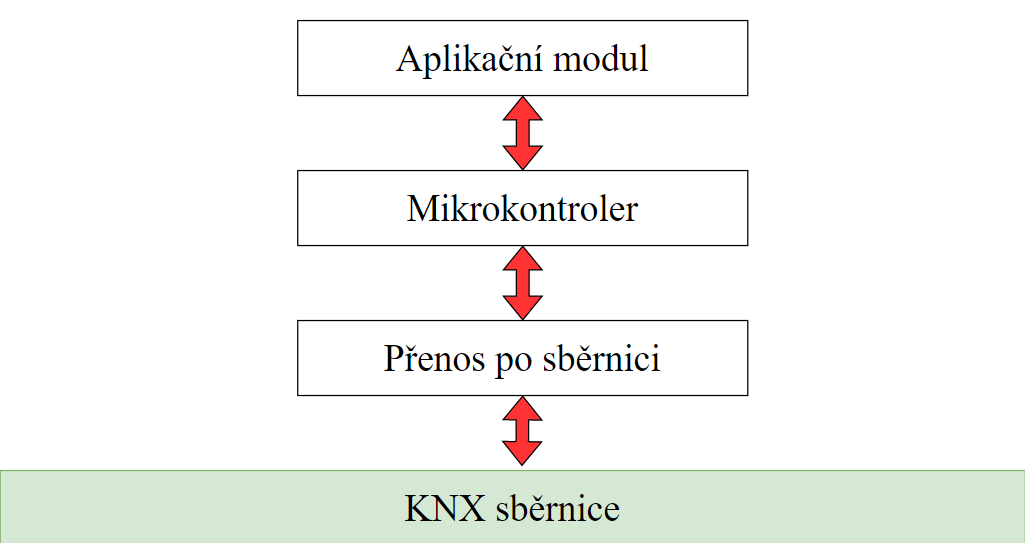
\includegraphics[scale=0.7]{obrazky/sbernice.png}
  \end{center}
  \caption[Součásti sběrnicového přístroje \cite{KNX principles}] {Součásti sběrnicového přístroje \cite{KNX principles}}
  \label{fig:Součásti sběrnicového přístroje}
\end{figure}
Přístroje lze ještě dělit na aktivní a pasivní. Pasivní přístroje nejsou součástí ICT, ale jedná se o podpůrné přístroje určené pro podporu procesu. Ve zkratce to znamená, že nekomunikují s ostatními přístroji. Jedním z příkladů pasivních přístrojů jsou napájecí zdroje.  Příkladem pasivních přístrojů jsou napájecí zdroje (Napájecí zdroje mohou být rozšířené ještě o ICT, ale není to časté).  
Aktivní přístroje lze rozdělit do těchto kategorií \cite{KNX principles}:
\begin{itemize}
\item Rozhraní - propojuje sběrnici a PC
\item Spojky - Optimalizují komunikaci v systému
\item Snímače - Předávají informace sběrnicovému systému
\item Akční členy - propojují klasické spotřebiče se sběrnicovým systémem
\end{itemize}

\subsection{Adresování}
\label{Adresování}
Individuální adresa je v instalaci jedinečná, tj. neexistuje další stejná adresa a požívá se k přesné identifikaci přístroje na sběrnici. Adresa je 16-bitová a je rozdělená na tři části (viz Obr. \ref{fig:Struktura individuální adresy]}).
\begin{figure}[!h]
  \begin{center}
    
\includegraphics[scale=0.6]{obrazky/Adresovani.png}
  \end{center}
  \caption[Struktura individuální adresy \cite{Celkovy prehled)}]{Struktura individuální adresy \cite{Celkovy prehled}}
  \label{fig:Struktura individuální adresy]}
\end{figure}

Nastavování individuální adresy na přístroji probíhá většinou stiskem programovacího tlačítka na přístroji. Při stisknutí tlačítka se rozsvítí programovácí LED. Individuální adresa se přístroji přiděluje natrvalo. Po přidělení již ETS posílá příslušná data (aplikace, konfigurace, parametry, skupinové adresy).

Při uvedení do provozu komunikace probíhá pomocí skupinových adres. Jedná se o adresy definované programátorem pro každou funkci v systému. Celkově je možno použít 65535 adres s tím, že adresa 0/0/0 je rezervována pro tzv. broadcast (Hlášení všem přístrojům na sběrnici). Programátor si také může zvolit, kterou z uvedených struktur použije (viz Obr. \ref{fig:Příklad struktury skupinových adres}). 
\begin{figure}[!h]
  \begin{center}
    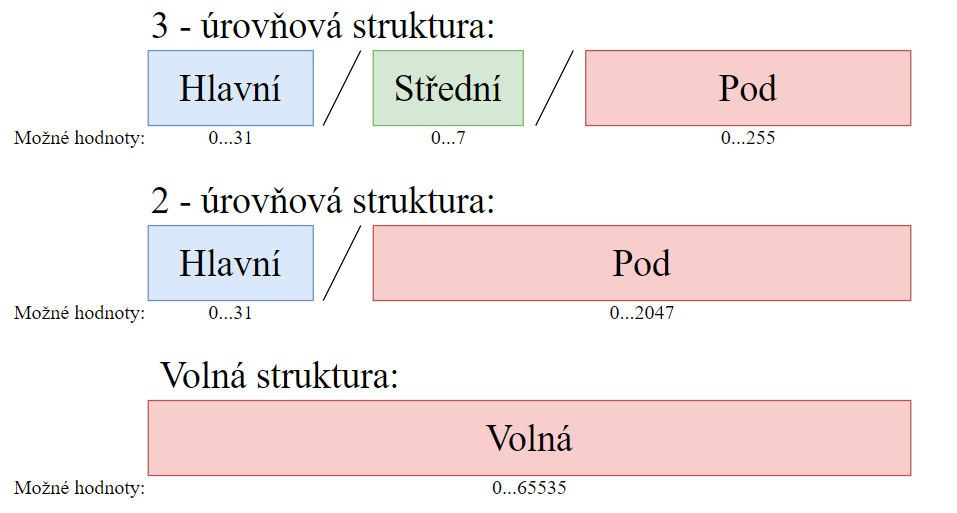
\includegraphics[scale=0.6]{obrazky/Skupinove adresovani.png}
  \end{center}
  \caption[Příklad struktury skupinových adres \cite{Celkovy prehled}]{Příklad struktury skupinových adres \cite{Celkovy prehled}}
  \label{fig:Příklad struktury skupinových adres}  
\end{figure}
Nejčastěji se využívá třístupňová struktura kvůli přehlednosti. Hlavní skupina se používá na číslo podlaží,  střední skupina na funkci (např. 1 = osvětlení, 2 = topení, 3 = stínění etc.)a podskupina pro konkrétní spotřebič, nebo skupinu spotřebičů. \cite{Celkovy prehled}
\\
\\
\\
\subsection{Komunikace}
Komunikace přístrojů na sběrnici probíhá pomocí tzv. telegramů (viz Obr. \ref{fig:Struktura telegramu}), kde je délka dat závislá na typu datového bodu  (1bit - 14bytů).
Nejdůležitější části telegramu jsou tři bloky \cite{Celkovy prehled}:
\begin{itemize}
\item Zdrojová adresa - udává adresu přístroje který telegram vyslal
\item Cílová adresa - adresa přístroje, kterému je telegram určen
\item Užitečná data - příkaz co má daný přístroj vykonat\\
\end{itemize}
\begin{figure}[!h]
  \begin{center}
    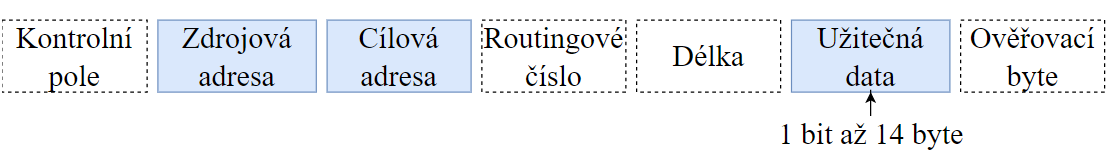
\includegraphics[scale=0.7]{obrazky/Struktura telegramu.png}
  \end{center}
  \caption[Struktura telegramu \cite{Celkovy prehled}]{Struktura telegramu \cite{Celkovy prehled}}
  \label{fig:Struktura telegramu}
\end{figure}
Telegramy na sběrnici čtou všechny přístroje, ale vykoná jej pouze přístroj určený cílovou adresou.

Komunikace na sběrnici probíhá pouze v případě, že je na sběrnici logická "1". V opačném případě je sběrnice přeplněná a pokračuje ve vysílá pouze přístroj s logickou "0" (viz Obr. \ref{fig:Struktura bitu kroucené dvojlinky}). \cite{Celkovy prehled}

\begin{figure}[!h]
  \begin{center}
    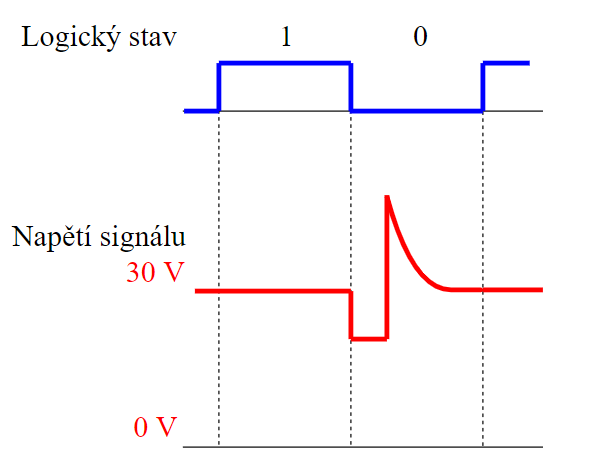
\includegraphics[scale=0.7]{obrazky/Struktura bitu.png}
  \end{center}
  \caption[Struktura bitu kroucené dvojlinky \cite{Celkovy prehled}]{Struktura bitu kroucené dvojlinky \cite{Celkovy prehled}}
  \label{fig:Struktura bitu kroucené dvojlinky}
\end{figure}

Aby jsme se vyhli kolizím a jeden z přístrojů mohl vysílat je přenos řízen principem CSMA/CA (Carrier Sense Multiple Access with Collision Avoidance vícenásobný přenos s vyhnutím se kolizím), který funguje tak, že pokud přístroj odesílající logickou “1” detekuje logickou “0”, aby se uvolnila cesta pro přenos jinému přístroji. Přístroj s přerušeným přenosem sleduje provoz na sběrnici a vyčká do konce přenosu jiného zařízení a poté zkusí znova vysílat. \cite{Celkovy prehled}

\subsection{Datový bod}
Datové typy byly standardizovány za účelem zajištění kompatibility podobných přístrojů od různých výrobců. Jedná se například o stmívání, žaluzie a hodiny. Standardizace zahrnuje požadavky na formát dat a strukturu komunikačních objektů snímačů a akčních členů. I tak existuje více druhů datových bodů (DPT) se stejnou funkcionalitou. Kombinace různých typů DPT se nazývají funkčními bloky.\cite{Celkovy prehled}
\\Skutečná informace datového bodu:
\begin{itemize}
    \item Není uložena v paměti zařízení.
    \item Není nikdy součástí telegramu
    \item Je pouze v projektu ETS\\
\end{itemize}
Typy datových bodů jsou zvláště důležité pro diagnostiku to znamená, že umožňují ETS monitorovat data spojená se skupinovými objekty, např. místo "data = 85 A8" je zobrazeno "data = -6 °C". \cite{Datapoint}\\
\\Struktura datového bodu a notace \cite{Datapoint}:
\begin{itemize}
    \item Datový typ : formát + kódování
    \item Velikost: rozsah hodnot + jednotky
\end{itemize}
Notace datového bodu se píše ve tvaru X.YYY, neboli DATOVÝ TYP.VELIKOST.

\begin{table}[h]
 \caption[Přehled nejpoužívanějších datových typů]{Přehled nejpoužívanějších datových typů}
   \small
    \centering
	  \begin{tabular}{|c|c|c|}
	    \hline
	    Značení & Formát  & Funkce  \\
	    \hline\hline
	    1.yyy & boolean & přepínání (001), krok (007),... \\
	    \hline
	    3.yyy & boolean + 3-bit unsigned & stmívání \\
	    \hline
	    5.yyy & 8-bit unsigned + 3-bit unsigned & stmívání(0-100\%), pozice rolet(0-100\%)\\
	    \hline
	    7.yyy & boolean + 3-bit unsigned & čitač pulsů \\
	    \hline
	    9.yyy & 16-bit float & přenos hodnoty teploty, jasu, rychlost větru \\
	    \hline
	    14.yyy & 32-bit float & nastavení teploty\\
	    \hline
	    19.yyy & čas + data & výstupy obrazovek \\
	    \hline
	    20.yyy & 8-bit enumerace & Topení, chlazení a ventilace ('komfort',...) \\
	    \hline
	  \end{tabular}
\end{table}

Díky existenci datového bodu jsme schopní nastavit hodnotu osvětlení 3 různými způsoby \cite{Systemove Argumenty}:
\begin{itemize}
    \item Zapnutí/Vypnutí
    \item Krokové stmívání - Při poslání telegramu "start stmívání" osvětlení krokově roste o definovanou hodnotu. Po poslání "stop stmívání" hodnota neroste.
    \item Procentuální stmívání- Realizuje se pomocí cyklického posílání telegramu. Při každém přijetí telegramu se zvedne jas o nastavenou hodnotu.
\end{itemize}

\section{Zabezpečení}
Rozdíl mezi zařízeními KNX a zabezpečenými KNX Secure je ten, že zařízení KNX Secure jsou schopna šifrovat a dešifrovat telegramy. Tato technologie dodává instalaci extra zabezpečení, a to během uvádění instalace do provozu, tak i poté za běhu. Telegramy jsou zašifrované zabezpečenými zařízeními KNX se nazývají zabezpečené telegramy.
\\Lze rozlišit dva typy šifrovaných telegramů KNX \cite{KNX Secure}:
\begin{itemize}
\item{Zcela zašifrované}
\begin{itemize}
\item{Lze použít pouze na zařízeních KNX IP a je označováno jako KNX IP Secure.}
\item{Používá se, pro zabezpečení části intalace, která je vystavená externí IP síti (typicky se jedná o páteřní linku).}
\end{itemize}
\item{Čatečně zašifrované}
\begin{itemize}
\item{Lze požít na libovolné komunikační zařízní KNX. Zařízení používající tento typ zabezpečení se nazývají KNX Data Secure}
\item{Toto šifrování můžeme použít i pro KNX IP, ale pouze pro tu část instalace, která není vystavena externí IP síti.}
\end{itemize}
\end{itemize}
Oba typy zabezpečení obsahují MAC (Message Authentication Code).
\\Zabezpečená zařízení mají zabezpečený režim, který je v projektu ETS reprezentován vlastností nazvanou „Secure Commissioning“. Pouze když je tento režim aktivován, zařízení je schopno šifrovat a dešifrovat telegramy.

Zabezpečená zařízení mají tzv. "Tool Key". V moment, když je aktivován zabezpečený režim zařízení, je ETS schopen komunikovat s tímto zařízením pouze pokud zná Tool Key tohoto zařízení.

Zabezpečená zařízení obsahují také Factory Default Setup Key (FDSK). FDSK je jedinečný pro každé zařízení a nelze jej upravovat ani mazat. ETS tento klíč může načíst jenom pomocí certifikátu (25znakový kód, který obsahuje sériové číslo a FDSK). Tool Key je v zásadě z výroby nastaven na FDSK. Tool Key může být také zpětně nastaven na FDSK pomocí tzv. "master resetu", který uvadí výrobce. 

Po přidání zabezpečeného zařízení KNX  do ETS a po přidání jeho certifikátu, ETS automaticky nastaví svůj Tool Key v projektu. To znamená, že uživatel ETS nemůže definovat/upravit Tool Key ručně, Tool Key také není viditelný pro uživatele ETS. \cite{KNX Secure}

\section{Topologie}
Základním kamenem topologie je hlavní linie, na kterou lze připojit až 256 přístrojů (účastníků sběrnice - US). Tato linie lze rozdělit až na 15 dalších segmentů za použití liniových opakovačů/spojek (LS). Na takto vzniklé segmenty (linie) připojit dalších 256 US. To vše ovšem závisí také na spotřebě přístrojů použitých v instalaci. To znamená, že celková spotřeba všech přístrojů nesmí překročit jmenovitý proud na druhé straně sběrnicového zdroje, který každá linie musí mít vlastní. Také lze mít maximálně 4 000 US na celé topologii. Toto množství lze také navýšit za použití oblastní spojky (OS) díky na páteřní linii. Po připojení vznikne tzv. nadřazená páteřní linie, která může pojmout až 16 oblastních spojek a celek rozdělí na dílčí páteřní linie. Celkový počet US na takovéto linii může být až 61 000. Reálné množství je v tomto případě omezeno zdrojem s tlumivkou (NZ/TI). \cite{Topologie}\\\\
Pro sběrnici KNX lze použít pouze tyto struktury kabeláže:
\begin{itemize}
    \item Hvězdicová
     \item Liniová
     \item Stromová
     \item Kombinace výše uvedených\\ \\ \\
\end{itemize}
\begin{figure}[!h]
  \begin{center}
    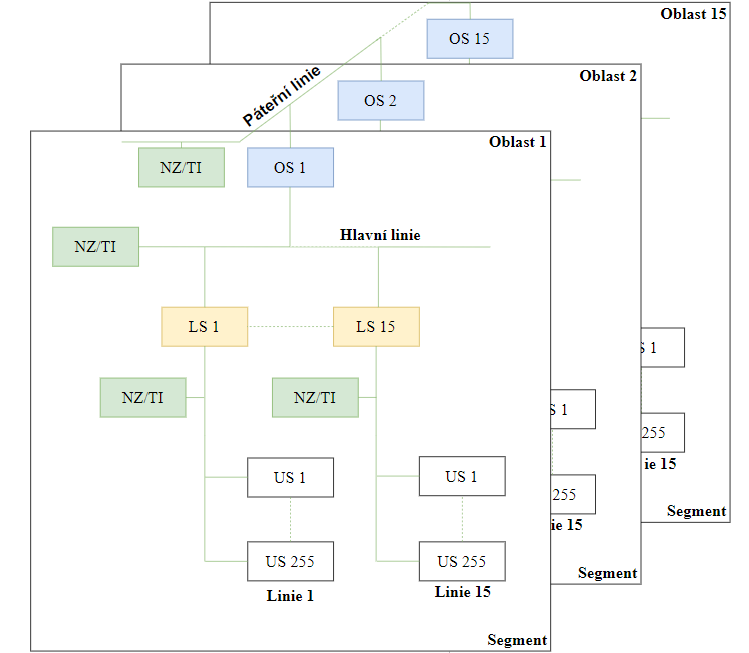
\includegraphics[scale=0.6]{obrazky/Ukazka topologie.png}
  \end{center}
  \caption[Ukázka topologie KNX\cite{Topologie}]{Ukázka topologie KNX\cite{Topologie}}
  \label{fig:Ukázka topologie KNX}
\end{figure}

\newpage
\subsection{Individuální adresa}
Individuální adresa se nastavuje s ohledem na umístění v topologii (Viz. Podkapitola \ref{Adresování}).
\begin{table}[h]
 \caption[Individuální adresy v topologii \cite{Topologie}]{Individuální adresy v topologii \cite{Topologie}}
   \small
    \centering
	  \begin{tabular}{|c|c|c|}
	    \hline
	    Prvek & Adresa & Funkce  \\
	    \hline\hline
	    Oblast & 0 & adresuje účastníky v páteřní linii \\
	    \hline
	    Oblast & 1...15 & adresuje oblasti \\
	    \hline
	    Linie & 0 & adresuje hlavní linii příslušné oblasti \\
	    \hline
	    Linie & 1...15 & adresuje linie obsažené v oblasti\\ 
	    \hline
	    Účastník na sběrnici & 0 & adresuje liniovou spojku příslušné linie \\
	    \hline
	    Účastník na sběrnici & 1...255 & adresuje sběrnicové přístroje obsažené v linii \\
	    \hline
	  \end{tabular}
\end{table}
\newpage
\subsection{Spojka}
V případě,že jsou v instalaci použity spojky a mají přiřazeny správné individuální adresy, budou při projektování v programu ETS (Kapitola \ref{ETS}) automaticky vytvořeny filtrační tabulky jednotlivých spojek. Filtrační tabulka obsahuje skupinové adresy, které smí projít skrz příslušnou spojku (obsahuje všechny obsažené skupinové adresy, které adresují SU umístěné za spojkou). Tudíž každá linie pracuje nezávisle.

 Spojky jsou vytvořeny pro montáž na DIN lištu, kde se připojují primární i sekundární linie pomocí sběrnicové svorkovnice. Primární linie také funguje, jako napájení mikrokontroleru a při výpadku sítě ohlásí tuto skutečnost na sekundární linii. Jednou z výhod pojky je možnost programování z obou linií. Obsahují také žluté signalizující LED, které blikají pouze v případě, že spojka propustí telegram na příslušnou linii. Další vlastností spojky je galvanické oddělení mezi primární a sekundární linií. Poslední vlastností spojky je možnost přeměny na liniový opakovač. Opakovač se rozliší od spojky absencí nuly na konci individuální adresy (X.X.1 apod.). Využívá se pro rozšíření linie o další segment s 64 US. Tento úsek je limitován délkou kabelu, který může měřit maximálně 1000m. \cite{Topologie}
 
\subsection{Routingové číslo}
Každý telegram, který je vyslán přístrojem na obsahuje routingové číslo, které začíná na hodnotě 6. Toto číslo při každém průchodu spojkou, či opakovačem se dekrementuje dokud nedosáhne nulové hodnoty. Tuto vlastnost berou filtrační tabulky v potaz.
Pokud se jedná o servisní telegram, tak routingové číslo má hodnotu 7, která se při průchodu spojkou nedekrementuje. \footnote{Spojky vyrobeny po roce 2019 mají schopnost tuto hodnotu dekrementovat}. Tuto skutečnost berou v potaz i filtrační tabulky, které toto číslo ignorují, a tudíž všechny spojky tento telegram propustí. Tento telegram se vždy dostane k požadovanému účastníku bez ohledu na umístění.
Toto číslo také brání zasmyčkování (nekonečnému kolování) telegramu. \cite{Topologie}
\subsection{Interní a externí rozhraní}
Systém KNX je otevřený jiným systémům za použití vhodných rozhraní umístěných na libovolné linii (většinou se jedná o páteřní linii). Lze připojit například programovatelný logický automat (PLC), digitální síť integrovaných služeb (ISDN), systémová technika budov, internet a mnohé další.
Tato rozhraní přenáší obousměrně zprávy, které převede na komunikační protokol.

Nejedná se ovšem jenom o spojovaní KNX s externími médii, ale je možno spojit různá KNX média mezi sebou (např. spojení TP a RF). Existuje také možnost připojení částí instalace skrze optická vlákna. Tohle spojení přináší řadu výhod zejména galvanické oddělení celků a zvýšení celkové délky vedení. \cite{Topologie}

\chapter{ETS}
\label{ETS}
Jedná se o konfigurační softwarový nástroj, který je nezávislý na výrobci pro navrhování, konfiguraci inteligentních instalací, a také pro řízení budov pomocí systému KNX. Tento software funguje pouze na počítačových platformách využívajících operační systém Windows. \cite{ETS Kecy}.

\noindent Pomocí softwaru lze \cite{Mitrenga}:
\begin{itemize}
    \item \textbf{Vkládat katalogové produkty do projektu} -- Produkty schválené asociací KNX jsou obsaženy v katalogu a lze je použít v projektu. Produkty lze také přidávat manuálně prostřednictvím aplikačních programů s koncovkou ".knxprod".
    \item \textbf{Vytvořit architekturu objektu} -- rozdělit objekt na celky(budovy, patra, místnosti,...)
    \item \textbf{Parametrizace produktů}
    \item \textbf{Vytváření skupinových adres}
    \item \textbf{Nahrávání řešení projektu do přístrojů}
    \item \textbf{Vzdálené ovládání připojeného projektu}
    \item \textbf{Diagnostika}
    \item \textbf{Vytvoření dokumentace}
\end{itemize}

\section{Tvorba instalace}
Při vytváření projektu byl zvolen typ páteřní linie na IP, skupinové adresy byly zvoleny třístupňové a topologie typu TP. TP topologie byla použita i při tvorbě panelu.

Po úspěšném založení projektu se program přepnul do pracovní části, která je složená z osmi oken \cite{Mitrenga}:
\begin{itemize}
    \item \textbf{Budovy} - rozdělení objektu na celky
    \item \textbf{Skupinové adresy} - vytvoření a přiřazení skupinových adres přístrojům
    \item \textbf{Topologie} - zobrazení rozložení vytvořeného projektu v topologii
    \item \textbf{Kořeny projektu} - zobrazení všech oken kde se pracovalo
    \item \textbf{Přístroje} - seznam přístojů v projektu
    \item \textbf{Zprávy} - okno zaměřené na tvorbu dokumentace projektu
    \item \textbf{Katalog} - vyhledání a vložení produktů do projektu
    \item \textbf{Diagnostika} - okno určené pro otestování instalace\\
\end{itemize}

Pro vytvoření pracovního prostoru bylo použito okno \textit{budova}. Prostor byl pojmenován \textit{Demonstrativní panel} a byl rozdělen na pět logických celků. Tyto celky reprezentují pokoje zobrazené na panelu (vchod, kuchyň, koupelna, obývací pokoj a rozvaděč umístěný v zadní části panelu). Toto rozdělení bylo vytvořeno za účelem zvýšení přehlednosti objektu a následné ulehčení propojování přístrojů mezi sebou. Je nutno také dodat, že vytvoření jedné místnosti je podmínkou pro vkládání přístrojů do pracovní plochy.

Pro vložení přístrojů bylo nutno otevřít okno katalog, který ovšem neobsahoval použité přístroje. Kvůli této komplikaci bylo nutno navštívit webové stránky výrobců a následné stažení aplikačních programů. Tyto programy byly importovány do katalogu pomocí tlačítka \textit{Import...}. Vzhled projektu po přidání přístrojů lze vidět na Obr. \ref{fig:Projekt budovy v ETS}.

\begin{figure}[!h]
  \begin{center}
    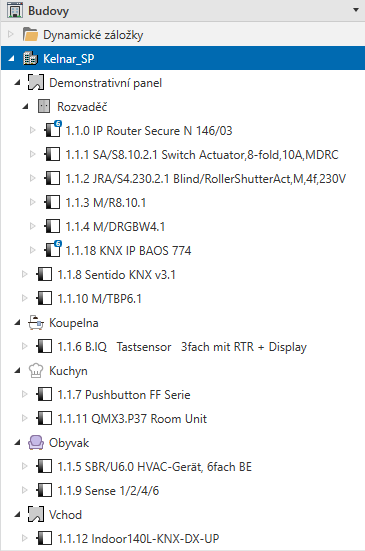
\includegraphics[scale=0.7]{obrazky/Budova.png}
  \end{center}
  \caption[Projekt budovy v ETS]{Projekt budovy v ETS}
  \label{fig:Projekt budovy v ETS}
\end{figure}

Po přidání všech přístrojů se zobrazila pracovní plocha, která slouží k zobrazení přehledu všech přístrojů (Zabezpečení - KNX Secure, individuální adresa prvku, místnost v projektu, použitý aplikační program, stav přístroje - nahrána adresa, program, parametrizace, skupinová adresa a informace o produktu). Ve sloupcích vyjadřujících stav přístroje jsou většinově pomlčky, které znázorňují, že nebyly nahrány všechny části do přístrojů. Tahle skutečnost je zdůvodněná změnami parametrů a skupinových adres.

\begin{figure}[!ht]
  \begin{center}
    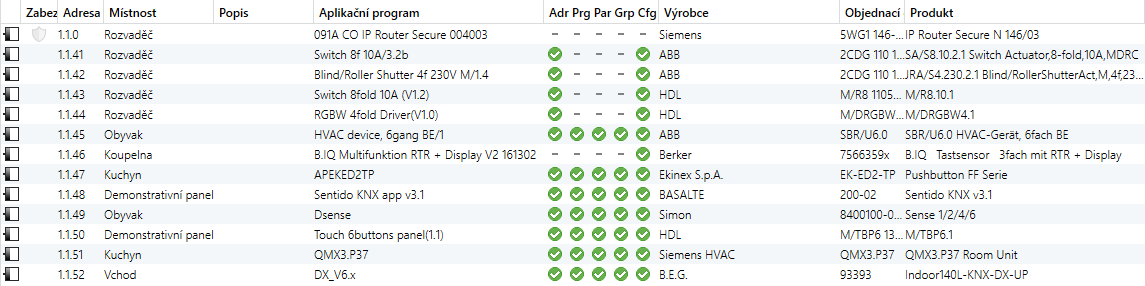
\includegraphics[scale=0.5]{obrazky/Přístroje v ETS.png}
  \end{center}
  \caption[Pracovní plocha v ETS]{Pracovní plocha v ETS}
  \label{fig:Pracovní plocha v ETS}
\end{figure}

\section{Parametrizace tlačítek a detektoru pohybu}
V této podkapitole je vysvětleno parametrizování použitých tlačítek. Ta byla pomyslně rozdělena do místností a nastavena, tak aby spolupracovala s nejbližšími prvky (světly, žaluziemi, klimatizací a topením), které jsou zobrazeny na Obr. \ref{fig:Vzheled panelu}. Pro vysvětlení byly vytvořeny tabulky popisu funkcí jednotlivých tlačítek. 

\begin{figure}[!h]
  \begin{center}
    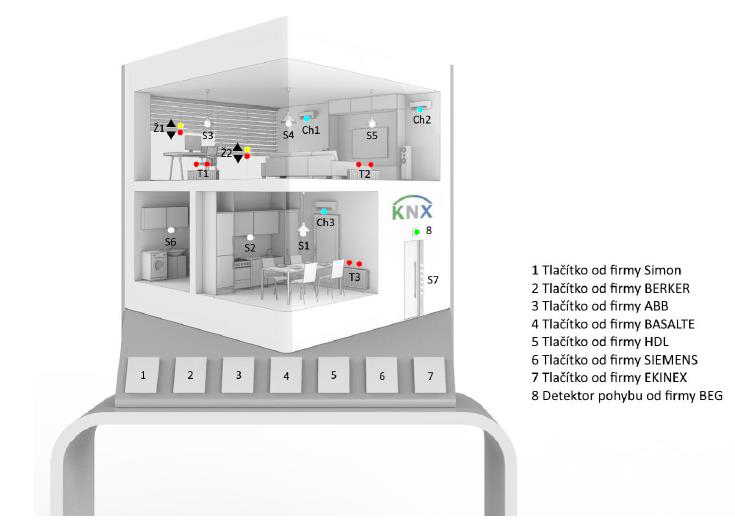
\includegraphics[scale=0.7]{obrazky/Panel_vzhled.png}
  \end{center}
  \caption[Grafický návrh panelu \cite{Mitrenga}]{Grafický návrh panelu \cite{Mitrenga}}
  \label{fig:Vzheled panelu}
\end{figure}

\subsection{ABB - SBR/U6.0.1-84}
Jedná se o šestinásobné tlačítko se zabudovaným termostatem, které lze použít na regulaci teploty, ovládání žaluzií, ovládání osvětlení a nastavení dvou scén, které mohou obsahovat až osm objektů. Každé stisknutí tlačítka změní barvu signalizační LED na předem stanovenou hodnotu (rozpoznání zapnuto/vypnuto). \cite{ABB}

\begin{figure}[!ht]
  \begin{center}
    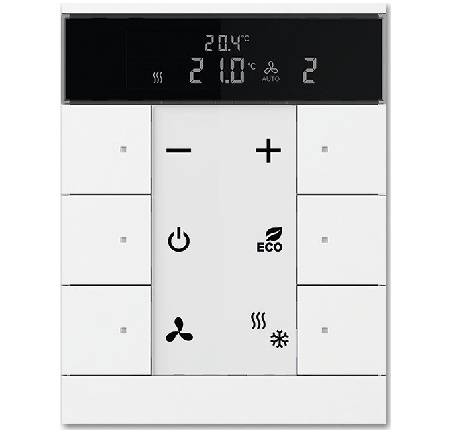
\includegraphics[scale=1.6]{obrazky/ABB.jpg}
  \end{center}
  \caption[Šestinásobné tlačítko s termostatem ABB - SBR/U6.0.1-84 \cite{ABB}]{Šestinásobné tlačítko s termostatem ABB - SBR/U6.0.1-84 \cite{ABB}}
  \label{fig:Šestinásobné tlačítko s termostatem ABB SBR/U6.0.1-84}
\end{figure}
Tlačítko bylo nastaveno na odesílání aktuální hodnoty teploty každých deset minut. Tlačítka jsou rozložena po horizontálních párech s označením funkční blok 1 až 3. V záložce každého bloku byla nastavena obě tlačítka na krátká a dlouhá stisknutí. V záložkách  \textit{Common parameter} byl vybrán typ objektu na 1-bit. Při krátkém stisknutí tlačítko odesílá hodnotu 1, při dlouhém stisknutí posílá hodnotu 2. Následně v záložce \textit{Extended parameters} byly nastaveny hodnoty odesílaných objektů u dlouhého stisknutí na on ("1") a u krátkého na off ("0").
V záložkách \textit{LED Button} pro každý funkční blok byla každá dioda nastavena do modu status. Přijímaný objekt byl nastaven na 1-bit a hodnota jasu na \textit{bright} signalizační barvu LED diod, tedy bílou při vypnutí a červenou při zapnutí. 
\subsection{Berker - 75663593}
Osminásobné tlačítko s termostatem by mělo být schopno regulovat pokojovou teplotu, ovládat žaluzie, ovládat osvětlení a scény. V této práci se ovšem nepovedlo nastavit ani při použití více zařízení a softwaru od Berkeru, který dokázal otevřít externí okno parametrizace v německém jazyce. Po ukončení parametrizace se parametry neuloží. \cite{Berker}
\begin{figure}[!ht]
  \begin{center}
    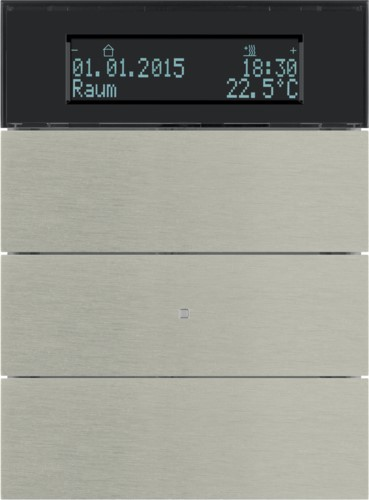
\includegraphics[scale=1.3]{obrazky/Berker.jpg}
  \end{center}
  \caption[Osminásobné tlačítko Berker - 75663593 \cite{Berker}]{Osminásobné tlačítko - Berker - 75663593 \cite{Berker}}
  \label{fig:Osminásobné člačítko s termostatem Berker 75663593}
\end{figure}
\newpage
\subsection{Ekinex - EK-ED2-TP-RW}
Jedná se o čtyřnásobné tlačítko se zabudovaným teplotním senzorem pro ovládání žaluzií, osvětlení a scén. \cite{Ekinex}

\begin{figure}[!ht]
  \begin{center}
    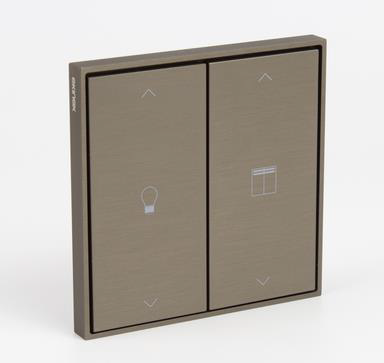
\includegraphics[scale=0.6]{obrazky/Ekinex.png}
  \end{center}
  \caption[Čtyřnásobné tlačítko Ekinex - EK-ED2-TP-RW \cite{Mitrenga}]{Čtyřnásobné tlačítko Ekinex - EK-ED2-TP-RW \cite{Mitrenga}}
  \label{fig:Čtyřnásobné tlačítko se zabudovaným teplotním senzorem Ekinex - EK-ED2-TP-RW}
\end{figure}

Tlačítko bylo nastaveno v záložce \textit{General} na dvě svislé klapky. Obě klapky byly nastaveny na dlouhé a krátké stisknutí. V případě první klapky se horní krátký stisk nastavil na funkci \textit{toggle} (přepínání). Dlouhý stisk představuje funkci \textit{off}. Pro dolní část klapky, je nastavení přesně opačné. Druhá klapka je nastavená stejným způsobem, akorát místo funkce \textit{toggle} byla použita funkce \textit{none}. Tato funkce zasílá "0", což znamená u žaluzií pohyb směrem nahoru.

\subsection{Basalte - Senido 202-03}
Další z použitých snímačů je čtyřnásobné dotykové tlačítko se zabudovaným snímačem teploty pro ovládání žaluzií, osvětlení a scén. Toto tlačítko má rovněž schopnost rozlišovat krátké a dlouhé stisknutí, a to nejen na jednom segmentu, ale má možnost snímat více segmentů najednou (multitouch). Dokáže ovládat až šest scén s osmi objekty. Další ze schopností tlačítka je posílání tříbajtové hodnoty RGB. Poslední z funkcí tlačítka je zobrazování statusu díky RGB podsvícení. \cite{Basalte}

\begin{figure}[!ht]
  \begin{center}
    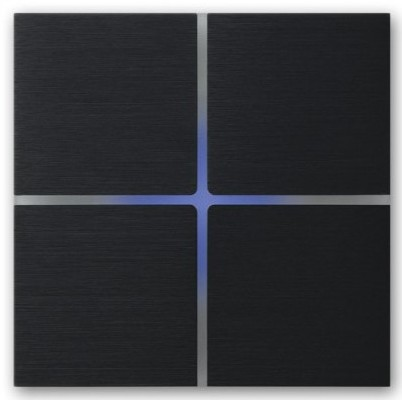
\includegraphics[scale=0.4]{obrazky/Basalte.jpg}
  \end{center}
  \caption[Čtyřnásobné dotykové tlačítko Basalte - Senido 202-03 \cite{Basalte}]{Čtyřnásobné dotykové tlačítko Basalte - Senido 202-03 \cite{Basalte}}
  \label{fig:Čtyřnásobné dotykové tlačítko Basalte - Senido 202-03}
\end{figure}

Tlačítko bylo rozděleno na čtyři samostatné zóny v záložce \textit{General}. Dále se v této záložce povolila funkce řadiče scén. První trojici tlačítek byla nastavena scéna, kterou budou při stisknutí volat.  Každá z těchto scén byla nastavena v korespondující záložce označené číslem. Poslední tlačítko bylo nastaveno na demonstraci schopnosti zasílat hodnoty RGB. Jedná se o 2 nastavené hodnoty, které se rozlišují délkou stisku. Pro demonstraci funkce multitouch byla vybrána funkce \textit{room toggle + General on/off/scene}. Pro krátký stisk byla vybrána scéna, která se zapne při krátkém stisku. Při druhém stisku se panel vypne. Dlouhý stisk má přiřazenou vlastní scénu. V záložce \textit{Temperature senzor} bylo nastaveno, aby senzor zasílal teplotu každých 5 minut. Záložka \textit{Scene controller}, která je určená pro nastavení řadiče scén, byla nastavena na všech výstupech na hodnotu 1-bit.

\subsection{Simon - 8400100-039}
Čtyřnásobné tlačítko se zabudovaným RGB podsvícením a teplotním senzorem pro ovládání žaluzií a osvětlení. \cite{Simon}

\begin{figure}[!ht]
  \begin{center}
    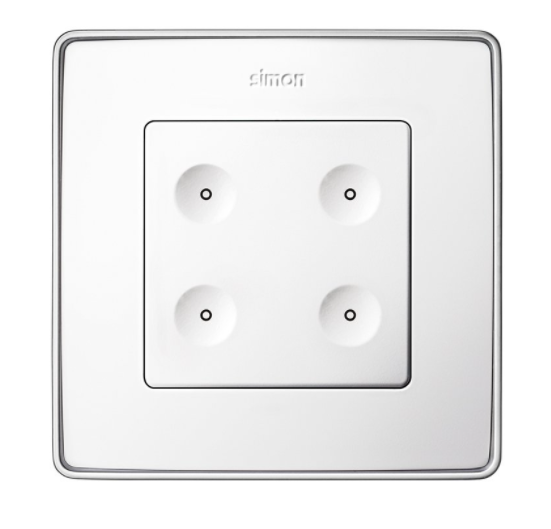
\includegraphics[scale=0.4]{obrazky/Simon.png}
  \end{center}
  \caption[Čtyřnásobné tlačítko Simon - 8400100-039 \cite{Simon}]{Čtyřnásobné tlačítko Simon - 8400100-039 \cite{Simon}}
  \label{fig:Čtyřnásobné tlačítko Simon - 8400100-039}
\end{figure}

V záložce \textit{General} bylo vybráno čtyř tlačítkové provedení, které je použito na demonstrativním panelu. Jako další možnost, která byla povolena, byl vnitřní senzor teploty. Poté v záložce \textit{FeedBack} byly nastaveny hodnoty jasu a hlasitosti na maximum. Dále zde byla aktivována možnost zpětné vazby doteku vibracemi. Pro nastavení samotné funkcionality tlačítek se musela použít záložka \textit{Inputs}, kde se nastavilo oddělení tlačítek od sebe (všechna tlačítka jsou samostatně). Tlačítka v tomto případě jsou číslována od spodního levého rohu po sloupcích (1 a 2 levá strana, 3 a 4 pravá strana). Poté už se nastavovala samotná funkcionalita tlačítek. Byla vybrána možnost krátkého i dlouhého stisku. V případě krátkého stisku žaluzie vyjedou/sjedou samostatně. Dlouhý stisk znamená pohyb pouze v čase, kdy je tlačítko stisknuto.

\subsection{HDL - M/TBP6.1-A2}
Předposlední tlačítko je od společnosti HDL. Jedná se o šestinásobné dotykové tlačítko se zabudovaným RGB podsvícením pro ovládání žaluzií, osvětlení, stmívání a ovládání dvou scén s deseti objekty. Dále také obsahuje RGB kontrolér, který dokáže posílat 3-byte hodnotu obsahující informace o intenzitě každé složky. \cite{HDL}

\begin{figure}[!ht]
  \begin{center}
    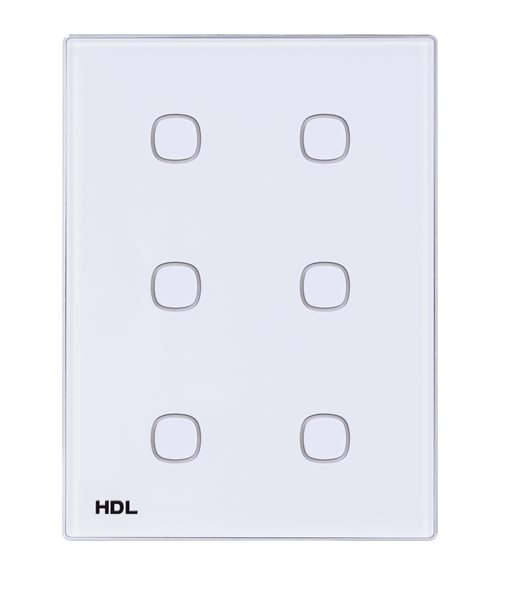
\includegraphics[scale=0.25]{obrazky/HDL.jpg}
  \end{center}
  \caption[Šestinásobné tlačítko HDL - M/TBP6.1-A2 \cite{HDL}]{Šestinásobné tlačítko HDL - M/TBP6.1-A2 \cite{HDL}}
  \label{fig:Šestinásobné tlačítko HDL - M/TBP6.1-A2}
\end{figure}

\newpage První z parametrů, které je možno nastavit v záložce \textit{General} byla citlivost dotyku, a to na hodnotu 4. Dále se pak povolily scény. Následně se obě scény nastaví v záložkáckách \textit{Panel scene A} a \textit{Panel scene B}. První scéna byla nastavena dle Obr. \ref{fig:Parametry scény A tlačítka HDL - M/TBP6.1-A2} a druhá dle Obr. \ref{fig:Parametry scény B tlačítka HDL - M/TBP6.1-A2}.

\begin{figure}[!ht]
  \begin{center}
    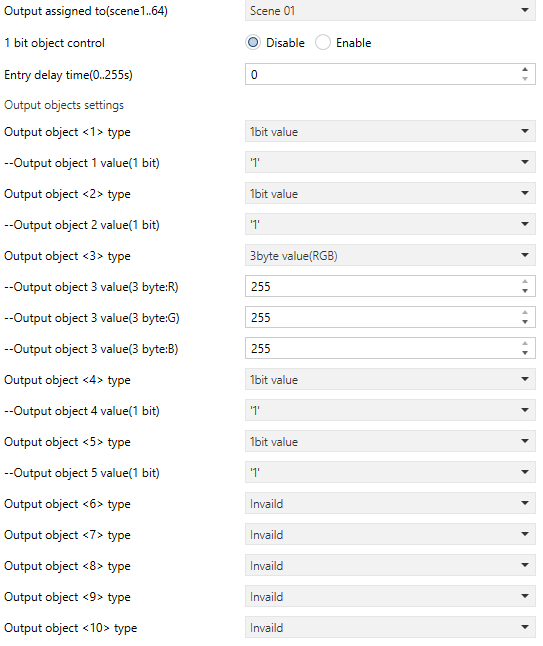
\includegraphics[scale=0.4]{obrazky/Scena A.png}
  \end{center}
  \caption[Parametry scény A tlačítka HDL - M/TBP6.1-A2]{Parametry scény A tlačítka HDL - M/TBP6.1-A2}
  \label{fig:Parametry scény A tlačítka HDL - M/TBP6.1-A2}
\end{figure}

\begin{figure}[!ht]
  \begin{center}
    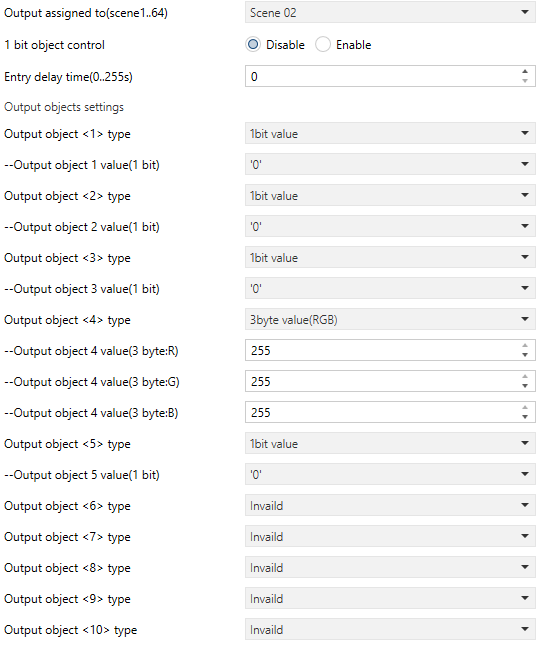
\includegraphics[scale=0.4]{obrazky/Scena B.png}
  \end{center}
  \caption[Parametry scény B tlačítka HDL - M/TBP6.1-A2]{Parametry scény B tlačítka HDL - M/TBP6.1-A2}
  \label{fig:Parametry scény B tlačítka HDL - M/TBP6.1-A2}
\end{figure}

Každé z těchto tlačítek má nastaveno signaliční podsvícení na jinou hodnotu. Krátkému stisknutí byla přiřazena funkce \textit{toggle}, která dovoluje přepínat osvětlení mezi hodnotami zapnuto a vypnuto. Dlouhé stisknutí bylo nastaveno na dobu 1s a používá se na stmívání. Pro demonstraci stmívání byly nastaveny různé hodnoty kroku prvních 4 tlačítek. Každé z těchto tlačítek má nastavenou signaliční podsvícení na jinou hodnotu. První tlačítko bylo nastaveno červenou barvu, druhou na zelenou, třetí na modrou a čtvrté na bílou. Při signalizaci se zvýší jas barev o 70\%. Zbylá 2 tlačítka byla přepnuta do modu RGB kontrolér, který odesílají hodnotu RGB jak pro krátké, tak i pro dlouhé stisknutí. Tato hodnota se také signalizuje při stisknutí tlačítek. 

\subsection{Siemens - QMX3.P37}
Jedná se o ovládací panel určený na regulování pokojové teploty s integrovaným displejem. Tento displej dokáže zobrazovat vlhkost vzduchu, koncentraci CO2 v ovzduší a samotnou teplotu místnosti. Také obsahuje osm tlačítek, která obsahují žluté statusové LED. Tento panel umožňuje také ovládání žaluzií, osvětlení a scény. \cite{Siemens}

\begin{figure}[!ht]
  \begin{center}
    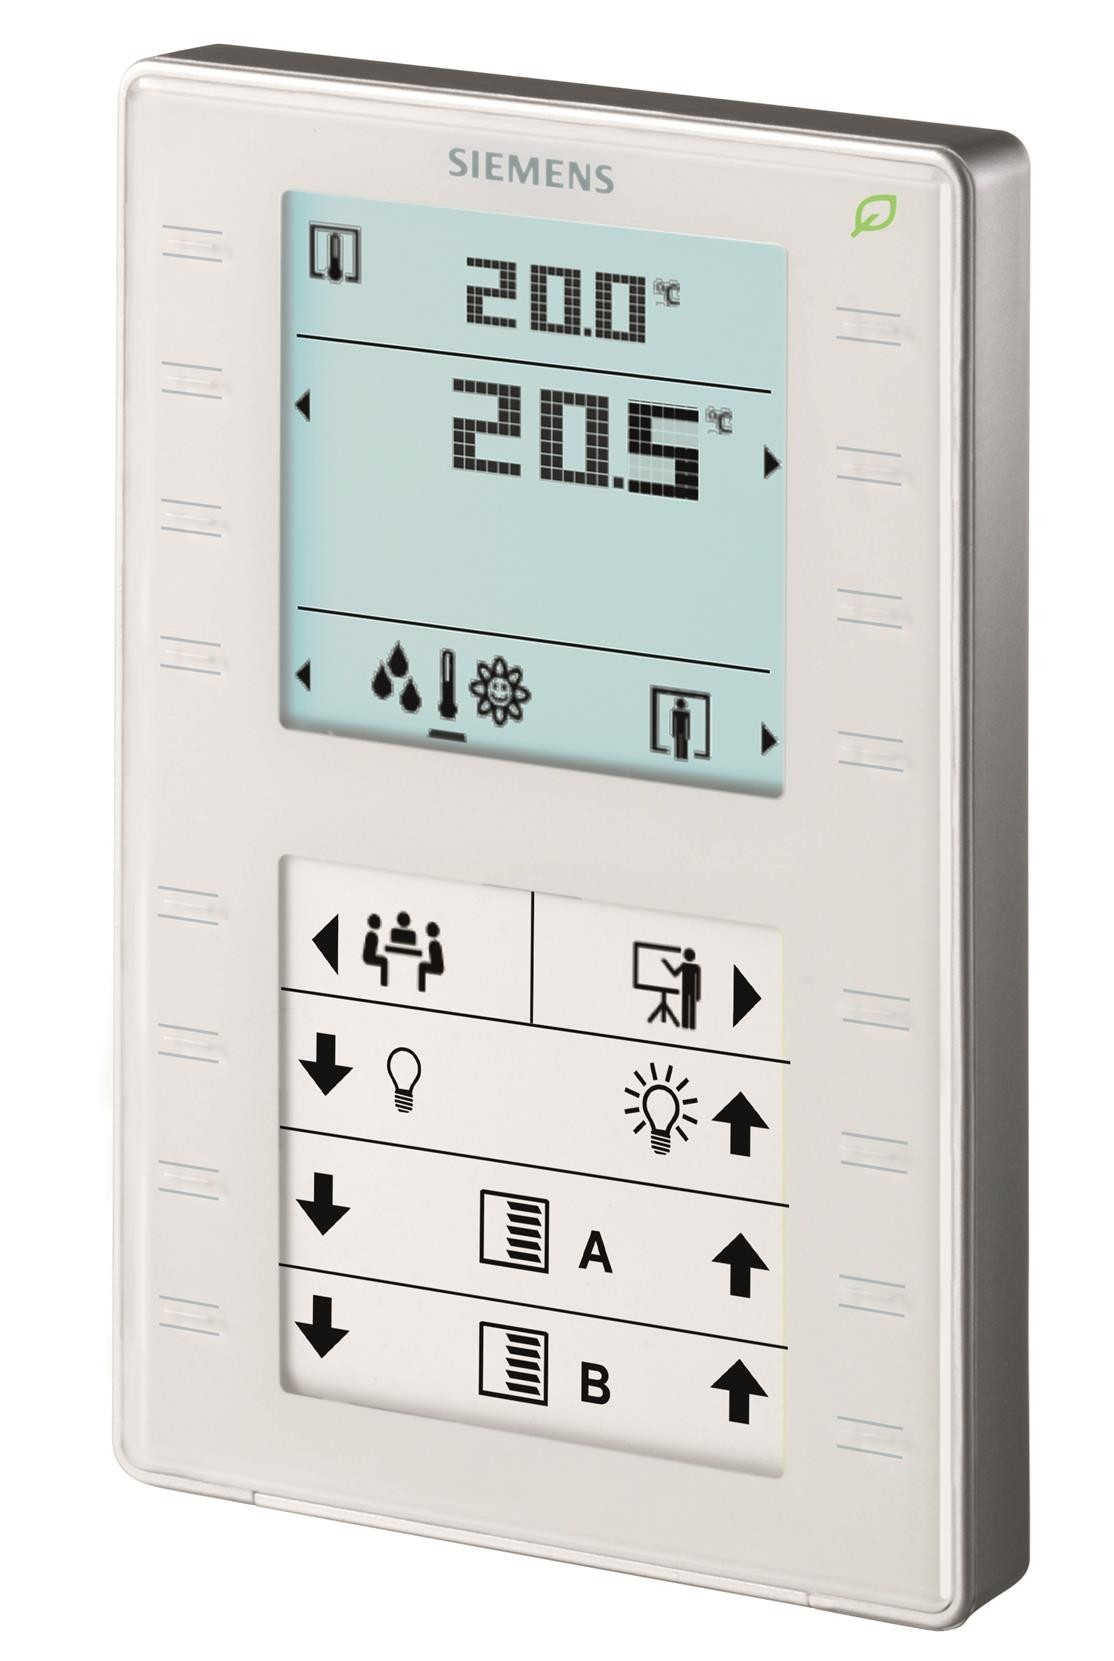
\includegraphics[scale=0.125]{obrazky/Siemens.jpg}
  \end{center}
  \caption[Ovladací panel Siemens - QMX3.P37 \cite{Siemens}]{Ovladací panel Siemens - QMX3.P37 \cite{Siemens}}
  \label{fig:Ovladací panel Siemens - QMX3.P37}
\end{figure}

V tomto případě bylo zařízení nastaveno na spínání pomocí jednoho tlačítka. Nejprve v záložce \textit{General} byla nastavena hodnota svitu signaližačnních LED na 100\% hodnotu. V další záložce byl nastaven teplotní senzor na odesílání hodnoty každých 10 minut. Poté se už nastavovaly jednotlivé tlačítkové páry. Funkce páru byla zvolena \textit{Individual}, která umožňuje nezávislé fungování obou tlačítek. Dále se u obou tlačítek nastavila možnost \textit{1 - button switching / send value}, \textit{Short/long press} (dlouhé stisknutí po uplynutí půl sekundy) a vybrala se možnost odesílání druhé hodnoty při dlouhém stisku. Levým tlačítkům byla přiřazena hodnota \textit{on} a pravým \textit{off}. Také byla nastavena signalizace stisku tlačítek. Kvůli tomu byla možnost \textit{LED display} nastavena na \textit{status object} a možnost \textit{LED activation} pro levá tlačítka na \textit{0 = LED off; 1 = LED on}. Pravá tlačítka byla nastavena \textit{0 = LED on; 1 = LED off}. Po pozdější úvaze o zefektivnění panelu se pro 1. a 4. řadu tlačítek změnil dlouhý stisk na \textit{Toggle}.  

\subsection{B.E.G - Indor 140-L-KNX-DX}
V první záložce \textit{Grundeinstellungen} (Základní nastavení) se nastavila hodnota teploměru (Temperaturmessung) na aktiviert. \cite{BEG}

Parametrizace tohoto prvku byla celá v němčině, a to dosti zkomplikovalo postup. První záložka \textit{Grundeinstellungen} (Základní nastavení) se nastavila hodnota teploměru (Temperaturmessung) na aktiviert. Poté v záložce teploměru se v možnosti zasílání teploty (\textit{Temperaturwer senden}) zvolilo odesílání při změně (bei Änderung). Další parametry byly nastaveny v záložce \textit{Tastenfunktionen} (Klíčové funkce), kde se aktivovala tlačítka T1 a T2. Nastavení \textit{Präsenzmelder} (Detektor pohybu) zůstalo v plně automatickém řežimu (\textit{Vollautomatik}). V první podzáložce detektoru pohybu byla nastavená doba vypnutí na 30 sekund. Při nastavování obou tlačítek byl vybrán režim spínání (\textit{Betriebsart}).

\begin{figure}[!ht]
  \begin{center}
    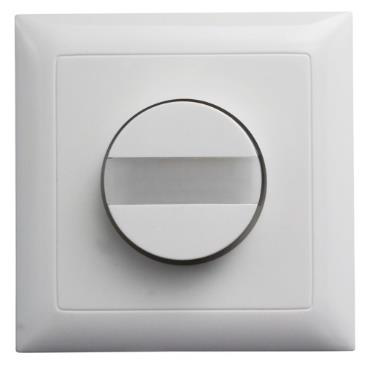
\includegraphics[scale=0.45]{obrazky/BEG.png}
  \end{center}
  \caption[Detektor pohybu B.E.G - Indor 140-L-KNX-DX \cite{Mitrenga}]{Detektor pohybu B.E.G - Indor 140-L-KNX-DX  \cite{Mitrenga}}
  \label{fig:Detektor pohybu B.E.G - Indor 140-L-KNX-DX }
\end{figure}

\section{Parametrizace akčních členů}
Tahle podkapitola se zaměřuje na parametrizaci použitých akčních členů umístěných v rozvaděči na zadní straně panelu.
\subsection{ABB SA/S8.10.2.1}
Tento osmikanálový spínací člen nebyl nijak parametrizován a byl ponechán ve stavu spínacího aktoru, který zasílá status pouze při změně. Úkolem tohoto aktoru je spínání LED představující topení a klimatizaci.

\begin{figure}[!ht]
  \begin{center}
    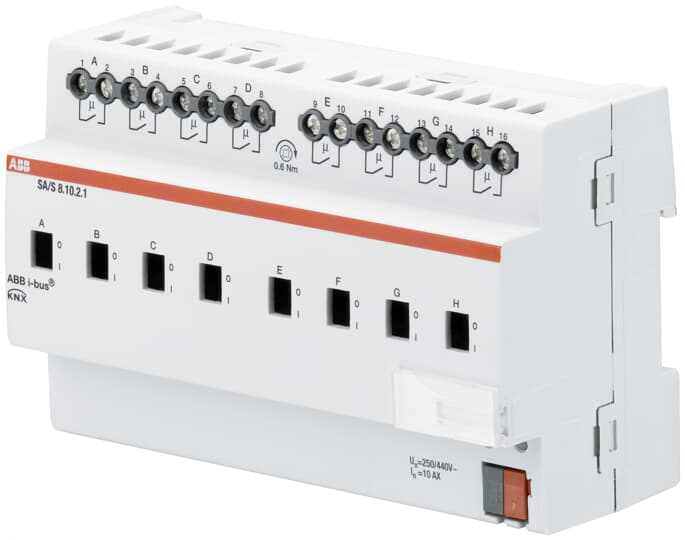
\includegraphics[scale=0.25]{obrazky/ABB aktor1.jpg}
  \end{center}
  \caption[Osmikanálový spínací člen ABB - SA/S8.10.2.1 \cite{ABB aktor1}]{Osmikanálový spínací člen ABB - SA/S8.10.2.1  \cite{ABB aktor1}}
  \label{fig:Osmikanálový spínací člen ABB - SA/S8.10.2.1}
\end{figure}

\subsection{ABB - JRA/S4.230.2.1}
Jedná se o čtyřkanálový žaluziový člen, který je určen k ovládaní žaluzií. Jelikož se v projektu používají pouze 2 žaluziové okruhy, tak se využívá pouze polovina akčního členu. Využívají se první dva kanály. Jediná změna od původní parametrizace je v záložkách \textit{Drive} pro jednotlivé kanály a to nastavení ukončení pohybu po 5 sekundách (tj. žaluzie může po stisku vyjíždět/sjíždět po dobu maximálně 5 sekund). 

\begin{figure}[!ht]
  \begin{center}
    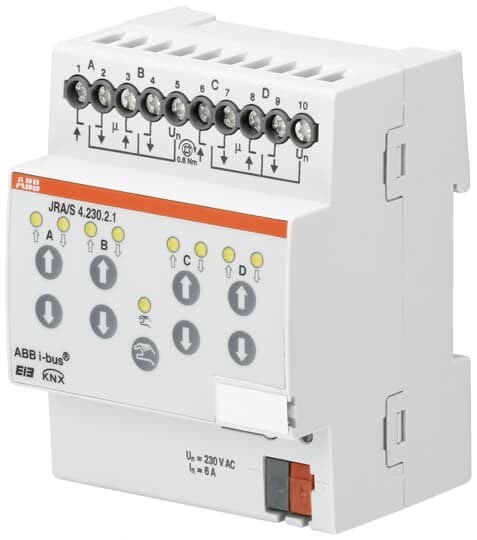
\includegraphics[scale=0.25]{obrazky/ABB aktor2.jpg}
  \end{center}
  \caption[Čtyřkanálový žaluziový člen ABB - JRA/S4.230.2.1 \cite{ABB aktor2}]{Čtyřkanálový žaluziový člen ABB - JRA/S4.230.2.1  \cite{ABB aktor2}}
  \label{fig:Čtyřkanálový žaluziový člen ABB - JRA/S4.230.2.1}
\end{figure}

\subsection{HDL - M/R8.10.1}
Osmikanálový spínací člen HDL se v této práci využívá ke spínání osvětlení tedy 7 LED, které představují osvětlení umístěné v domě. V tomto případě nebyla nutná žádná změna oproti původnímu nastavení parametrů. Všechny kanály jsou nastaveny jako spínací aktor s typem kontaktu Normally Opened (NO). Zasílání statusu probíhá pouze při změně hodnoty.

\begin{figure}[!ht]
  \begin{center}
    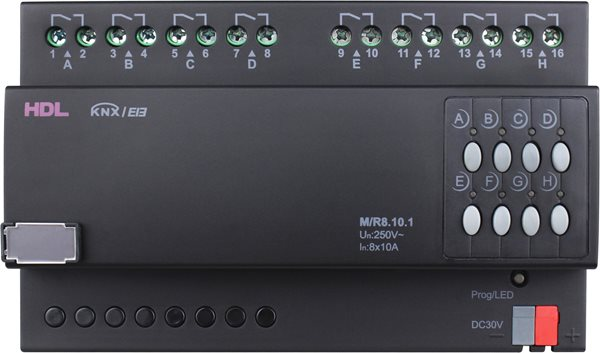
\includegraphics[scale=0.35]{obrazky/HLD aktor1.jpg}
  \end{center}
  \caption[Osmikanálový spínací člen HDL - M/R8.10.1 \cite{HDL aktor1}]{Osmikanálový spínací člen HDL - M/R8.10.1  \cite{HDL aktor1}}
  \label{fig:Osmikanálový spínací člen HDL - M/R8.10.1}
\end{figure}

\subsection{HDL - M/DRGBW4.1}
Čtyřnásobný stmívací člen poskytnutý společností HDL byl v této práci použit na ovládání RGBW LED pásku ukrytém v demonstrativním panelu. Výhodou tohoto členu je možnost ovládat kanál barevných složek zvlášť. Každý kanál (\textit{Channel}) je nastaven na odesílání stavové hodnoty (1bit) při změně. Dále se nastavily hodnoty času pro stmívání v záložkách \textit{dimming config} každého kanálu na 1 sekundu pro zapnutí i vypnutí. 

\begin{figure}[!ht]
  \begin{center}
    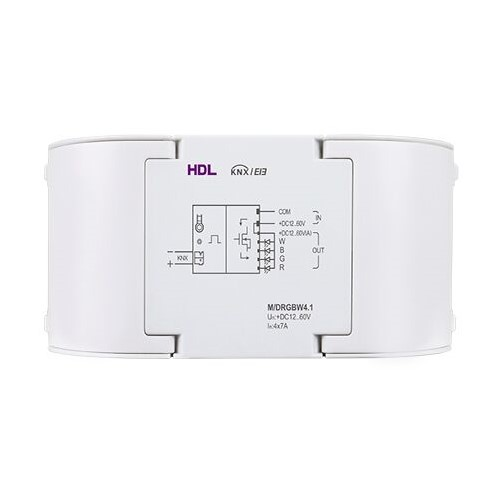
\includegraphics[scale=0.4]{obrazky/HLD aktor2.jpg}
  \end{center}
  \caption[Čtyřnásobný stmívací člen HDL - M/DRGBW4.1 \cite{HDL aktor2}]{Čtyřnásobný stmívací člen HDL - M/DRGBW4.1 \cite{HDL aktor2}}
  \label{fig:Čtyřnásobný stmívací člen HDL - M/DRGBW4.1}
\end{figure}

\section{Připojená komunikační rozhraní}
Pro umožnění parametrizace a externího řízení bylo nutno přidat do projektu dvě různá rozhraní pro komunikaci. První z nich je IP Secure router Siemens - 5WG1 146-1AB03, který je převážně určen k bezpečnému přenosu dat. Lze z něj také vytvořit liniovou spojku. \cite{Siemens IP}

Tomuto rozhraní byla pouze nastavena IP adresa, maska a základní brána pro komunikaci s RaspberryPi skrze tunelování.

\begin{figure}[!ht]
  \begin{center}
    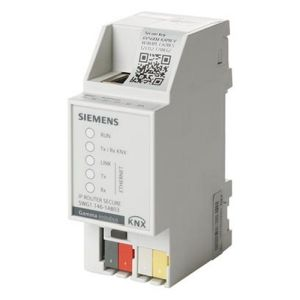
\includegraphics[scale=0.55]{obrazky/Siemens router.jpg}
  \end{center}
  \caption[IP Secure router Siemens - 5WG1 146-1AB03 \cite{Siemens IP}]{IP Secure router Siemens - 5WG1 146-1AB03 \cite{Siemens IP}}
  \label{fig:IP Secure router Siemens - 5WG1 146-1AB03}
\end{figure}

Druhé komunikační rozhraní použité na panelu je Weinzierl - KNX IP BAOS 774. Využívá se pro komunikaci skrze telegramy nebo datové body. Dále umožňuje přístup k objektům pomocí TCP/IP protokolu anebo za pomoci webového rozhraní. \cite{Weinzier}

Toto rozhraní bylo taktéž parametrizováno pro komunikaci s PLC. Byla mu nastavena odlišná IP adresa, stejná maska a brána jako u předchozího rozhraní. Dále se v něm definovaly datapointy pro komunikaci. Ty jsou definované v tabulce \ref{tab:Datapointy pro komunikaci KNX IP BAOS 774 s PLC}.

\begin{figure}[!ht]
  \begin{center}
    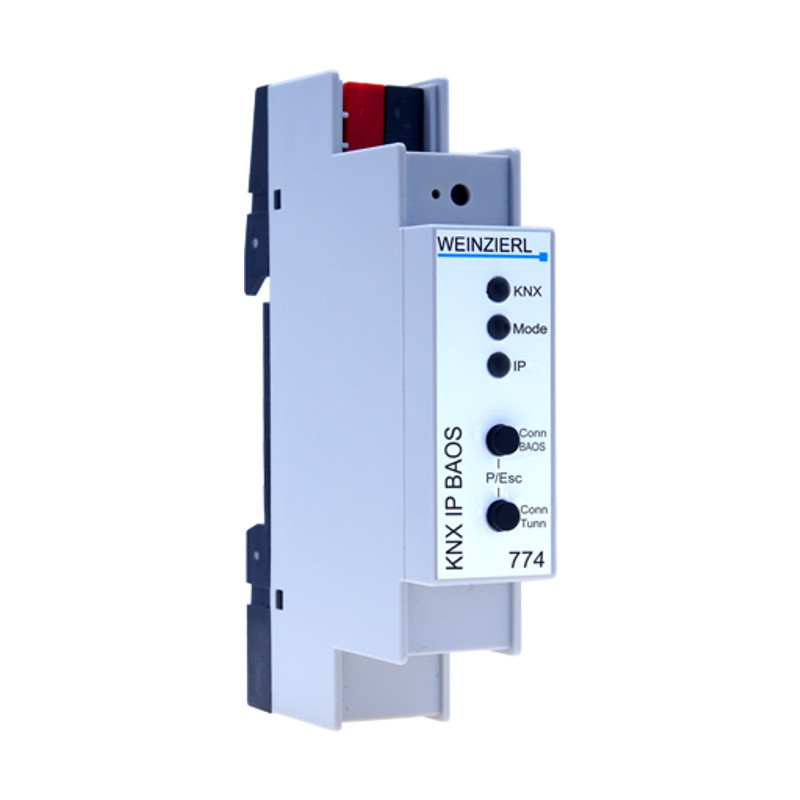
\includegraphics[scale=0.2]{obrazky/IP BAOS.jpg}
  \end{center}
  \caption[Komunikační rozhraní Weinzierl - KNX IP BAOS 774 \cite{Weinzier ob}]{Komunikační rozhraní Weinzierl - KNX IP BAOS 774 \cite{Weinzier ob}}
  \label{fig:Komunikační rozhraní Weinzierl - KNX IP BAOS 774}
\end{figure}
\pagebreak
\begin{table}[!ht]
  \caption[Datapointy pro komunikaci KNX IP BAOS 774 s PLC]{Datapointy pro komunikaci KNX IP BAOS 774 s PLC}
  \label{tab:Datapointy pro komunikaci KNX IP BAOS 774 s PLC}
  \small
    \centering
    \begin{tabular}{|c|c|c|}
      \hline
        Datapoint & Typ & Účel  \\
          \hline\hline
            1. & DPT 1 & Světlo pracovna zpětná vazba \\
          \hline
            2. & DPT 1 & Světlo obývací pokoj zpětná vazba \\
          \hline
            3. & DPT 1 & Světlo televize zpětná vazba \\
          \hline
            4. & DPT 1 & Světlo linka zpětná vazba \\
          \hline
            5. & DPT 1 & Světlo kuchyně zpětná vazba \\
          \hline
            6. & DPT 1 & Světlo koupelna zpětná vazba \\
          \hline
            7. & DPT 1 & Vchodové světlo zpětná vazba \\
          \hline
            8. & DPT 1 & Topení pracovna zpětná vazba \\
          \hline
            9. & DPT 1 & Topení televize zpětná vazba \\
          \hline
            10. & DPT 1 & Topení kuchyň zpětná vazba \\
          \hline
            11. & DPT 1 & Klimatizace pracovna zpětná vazba \\
          \hline
            12. & DPT 1 & Klimatizace televize zpětná vazba \\
          \hline
            13. & DPT 1 & Klimatizace kuchyně zpětná vazba \\
          \hline
            14. & DPT 1 & Levé žaluzie zpětná vazba \\
          \hline
            15. & DPT 1 & Levé žaluzie příkaz \\
          \hline
            16. & DPT 1 & Pravé žaluzie zpětná vazba \\
          \hline
            17. & DPT 1 & Pravé žaluzie příkaz \\
          \hline
            18. & DPT 1 & Světlo pracovna příkaz \\
          \hline
            19. & DPT 1 & Světlo obývací pokoj příkaz \\
          \hline
            20. & DPT 1 & Světlo televize příkaz \\
          \hline
            21. & DPT 1 & Světlo linka příkaz \\
          \hline
            22. & DPT 1 & Světlo kuchyně příkaz \\
          \hline
            23. & DPT 1 & Světlo koupelna příkaz \\
          \hline
            24. & DPT 1 & Vchodové světlo příkaz \\
          \hline
            25. & DPT 1 & Topení pracovna příkaz \\
          \hline
            26. & DPT 1 & Topení televize příkaz \\
          \hline
            27. & DPT 1 & Topení kuchyň příkaz \\
          \hline
            28. & DPT 1 & Klimatizace pracovna příkaz \\
          \hline
            29. & DPT 1 & Klimatizace televize příkaz \\
          \hline
            30. & DPT 1 & Klimatizace kuchyně příkaz \\
          \hline
            31. & DPT 1 & Krokování levé žaluzie \\
          \hline
            32. & DPT 1 & Krokování levé žaluzie \\
          \hline
            33. & DPT 18 & Scéna odchod \\
          \hline
            34. & DPT 9 & Teplota okolí panelu \\
          \hline
  \end{tabular}
\end{table}
\newpage
\section{Vytvoření skupinových adres projektu}
V závislosti na informacích obsažených v podkapitole \ref{Adresování} se tato podkapitola zaměří pouze na tvorbu skupinových adres. První část této podkapitoly bude věnována vytvoření a popsání tabulek jednotlivých místností. Tyto tabulky budou použity pro popis funkce jednotlivých tlačítek a následně pro tvorbu skupinových adres. Dále tyto tabulky nebudou obsahovat tlačítko společnosti Berker, které nelze parametrizovat.

První místnosti, které budou nastaveny, jsou kuchyně a koupelna. Do těchto prostor byly pomyslně nainstalovány tlačíka společnosti Ekinex a Siemens. Aby se využilo maximálně těchto tlačítek, budou využita obě tlačítka i v jiných místnostech. Zejména se jedná o tlačítko Ekinex, které má na pravé klapce žaluzie. V případě tlačítka Siemens se jedná pouze o využití velkého množství tlačítek, které budou použity při dlouhém stisku na ovládání celé budovy. 

\begin{table}[h]
 \caption[Funkce kuchyňských tlačítek pro krátké stisknutí]{Funkce kuchyňských tlačítek pro krátké stisknutí}
   \small
    \centering
	  \begin{tabular}{|c|c|c|}
	    \hline
	    Tlačítko & Ekinex & Siemens  \\
	    \hline\hline
	    1. & S1 Zapnuto/Vypnuto & Ch3 Vypnuto \\
	    \hline
        2. & S2 Zapnuto/Vypnuto & Ch3 Zapnuto \\
	    \hline
        3. & Ž1, Ž2 krok nahorů & T3 Vypnuto \\
	    \hline
        4. & Ž1, Ž2 krok dolů & T3 Zapnuto \\
	    \hline
        5. & - & T3/1 Vypnuto \\
	    \hline 
        6. & - & T3/1 Zapnuto \\
	    \hline 
	    7. & - & T3/2 Vypnuto \\
	    \hline
	    8. & - & T3/2 Zapnuto \\
	    \hline
	  \end{tabular}
\end{table}

\begin{table}[h]
 \caption[Funkce kuchyňských tlačítek při dlouhém stisknutí]{Funkce kuchyňských tlačítek při dlouhém stisknutí}
   \small
    \centering
	  \begin{tabular}{|c|c|c|}
	    \hline
	    Tlačítko & Ekinex & Siemens  \\
	    \hline\hline
	    1. & S1, S2, S6 Zapnuto/Vypnuto &  Ch1 Zapnuto/Vypnuto \\
	    \hline
        2. & S6 Zapnuto/Vypnuto &  Ch2 Zapnuto/Vypnuto \\
	    \hline
        3. &  Ž1, Ž2 nahorů & T1, T2, T2 Vypnuto \\
	    \hline
        4. & Ž1, Ž2 dolů & T1, T2, T2 Zapnuto \\
	    \hline
        5. & - &  Ch1, Ch2, Ch3 Vypnuto\\
	    \hline 
        6. & - & Ch1, Ch2, Ch3 Zapnuto \\
	    \hline 
	    7. & - & S1,S2,S6 Vypnuto \\
	    \hline
	    8. & - & S3,S4,S5 Zapnuto \\
	    \hline
	  \end{tabular}
\end{table}

\newpage Další místností se dvěma pomyslně nainstalovanými tlačítky je obývací pokoj. Jedná se o tlačítka společnosti ABB a Simon. Tlačítko Simon bude použito na ovládání žaluzií a tlačítko ABB na ovládání topení, chlazení a světel v místnosti.

\begin{table}[h]
 \caption[Funkce tlačítek obývacího pokoje při krátké stisknutí]{Funkce tlačítek obývacího pokoje při krátké stisknutí}
   \small
    \centering
	  \begin{tabular}{|c|c|c|}
	    \hline
	    Tlačítko & ABB & Simon  \\
	    \hline\hline
	    1. & T1 Vypnuto & Ž1 krok nahorů  \\
	    \hline
        2. & T2 Vypnuto & Ž1 krok dolů  \\
	    \hline
        3. & Ch1,Ch2 Vypnuto & Ž2 krok nahorů  \\
	    \hline
        4. & S3 Vypnuto & Ž2 krok dolů  \\
	    \hline
        5. & S4 Vypnuto & - \\
	    \hline 
        6. & S5 Vypnuto & - \\
	    \hline 
	  \end{tabular}
\end{table}

\begin{table}[h]
 \caption[Funkce tlačítek obývacího pokoje při dlouhém stisknutí]{Funkce tlačítek obývacího pokoje při dlouhém stisknutí}
   \small
    \centering
	  \begin{tabular}{|c|c|c|}
	    \hline
	    Tlačítko & ABB & Simon  \\
	    \hline\hline
	    1. & T1 Zapnuto & Ž1 nahorů  \\
	    \hline
        2. & T2 Zapnuto & Ž1 dolů  \\
	    \hline
        3. & Ch1,Ch2 Zapnuto & Ž2 nahorů  \\
	    \hline
        4. & S3 Zapnuto & Ž2 dolů  \\
	    \hline
        5. & S4 Zapnuto & - \\
	    \hline 
        6. & S5 Zapnuto & - \\
	    \hline 
	  \end{tabular}
\end{table}

Dotyková tlačítka společností Basalte a HDL byla určena na ovládání scén a barvy pozadí objektu. Tlačítko společnosti basalte v této práci reaguje pouze na  krátký dotek jednotlivých tlačítek. Tato skutečnost je způsobena použitím scén. Při použití funkce volání scény nelze využít dlouhého doteku. Další z vlastností tlačítka je již zmiňovaný multitouch, který funguje na bázi doteku dvou a více ploch najednou. V této práci je použit krátký dotek na zavolání scény odchod a dlouhý dotek na volání scény příchod.
\newpage
\begin{table}[!ht]
 \caption[Funkce dotykových tlačítek při krátké stisknutí]{Funkce dotykových tlačítek při krátké stisknutí}
   \small
    \centering
	  \begin{tabular}{|c|c|c|}
	    \hline
	    Tlačítko & Basalte & HDL \\
	    \hline\hline
	    1. & Scéna dovolená  & Červené podsvícení \\
	    \hline
        2. & Scéna léto  &  Zelené podsvícení \\
	    \hline
        3. & Scéna zima  & Modré podsvícení   \\
	    \hline
        4. & RGB Kontroler & Bílé podsvícení \\
	    \hline
        5. & - & Nastavená hodnota RGB 1 \\
	    \hline 
        6. & - &  Nastavená hodnota RGB 2 \\
	    \hline 
	  \end{tabular}
\end{table}

\begin{table}[!ht]
 \caption[Funkce dotykových tlačítek při dlouhém stisknutí]{Funkce dotykových tlačítek při dlouhém stisknutí}
   \small
    \centering
	  \begin{tabular}{|c|c|c|}
	    \hline
	    Tlačítko & Basalte & HDL  \\
	    \hline\hline
	    1. & - & Červené podsvícení stmívání  \\
	    \hline
        2. & - & Zelené podsvícení stmívání \\
	    \hline
        3. & - & Modré podsvícení stmívání  \\
	    \hline
        4. & - & Bílé podsvícení  stmívání \\
	    \hline
        5. & - & Nastavená hodnota RGB 3 \\
	    \hline 
        6. & - & Nastavená hodnota RGB 4 \\
	    \hline 
	  \end{tabular}
\end{table}

Poslední z použitých spínačů je detektor pohybu, kterému bylo logicky přiřazeno přední světlo domu.\\ \\Ze vzniklých tabulek byly vytvořeny skupinové adresy, které byly rozděleny do skupin dle přístroje (Světla, Žaluzie, Topení, Klimatizace, LED, Scény a Měření). Tyto skupiny se dále dělí podle funkcionality a množství. Poslední vrstva již představuje jednotlivé objekty nebo scény. Výpis skupinových adres je součástí příloh.
\chapter{Vizualizace skrze programovatelný logický automat}
\label{sec:vizualizace_automat}
V této kapitole se nachází popis jednotlivých částí ovládání instalace skrze PLC firmy TECO - CP-2007 \cite{TECO}, které obsahuje knihovny pro práci s KNX/IP \cite{KNXlib} a MQTT \cite{MQTTlib} a dále integrovaný webový server pro vizualizaci \cite{WebMaker}. Všechny tyto části jsou podrobněji rozvedeny v následujících podkapitolách.
Ovládání a vizualizace instalace je možné provádět i skrze PLC jiných výrobců za předpokladu, že mají implementované knihovny pro komunikace KNX/IP a MQTT. PLC výrobce TECO bylo vybráno díky jeho specializaci na domácí automatizaci, dostupnosti a ceně.
\section{CP - 2007}
Jedná se o základní modul řídícího systému Foxtrot v provedení s jednojádrovým procesorem ARMv7 o frekvenci 792MHz a databoxem o velikosti 128kB, který je vyroben pro přichycení na DIN Lištu. Obsahuje 2 ethernet porty, 2 sériové porty, 15 vstupů, z nichž je 14 univerzálních a 1 galvanicky oddělený digitální, 15 výstupů, z nichž je 11 releových a 4 analogové. Dále pak obsahuje 2 sloty na rozšiřující moduly. \cite{TECO}

\begin{figure}[!ht]
    \begin{center}
        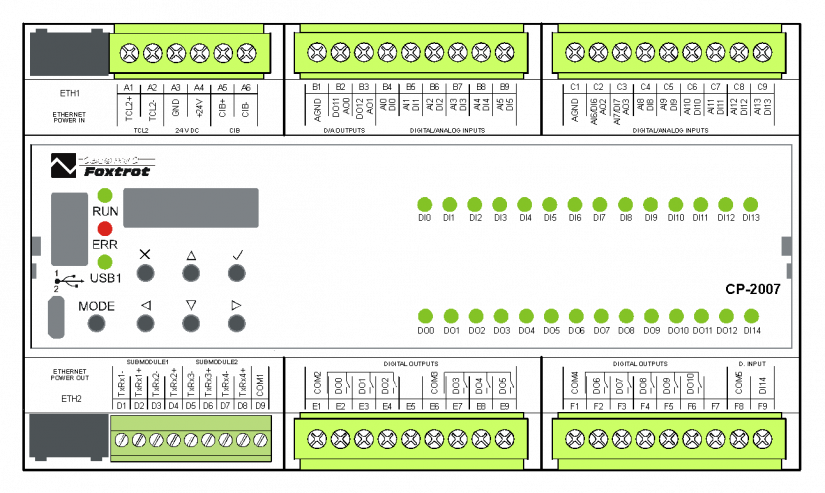
\includegraphics[scale=0.7]{obrazky/CP-2007.png}
    \end{center}
    \caption[CP-2007 \cite{TECO}]{CP-2007 \cite{TECO}}
    \label{fig:CP-2007}
\end{figure}

\section{Mosaic}
Ovládání instalace bylo realizováno v programovacím prostředí společnosti TECO - Mosaic, které je určeno pro programování PLC. Toto prostředí nabízí široké spektrum funkcí a nástrojů pro programování, vizualizaci a správu projektů \cite{Mosaic}: 

\begin{itemize}
    \item \textbf{Programovací jazyky dle IEC 61131-3 \cite{IEC61131-3}:}
        \begin{itemize}
            \item Ladder Diagram (LD)
            \item Function Block Diagram (FBD)
            \item Structured Text (ST)
            \item Instruction List (IL)
            \item Sequential Function Chart (SFC)
            \item Continuous Function Chart (CFC)
        \end{itemize}
    \item \textbf{Simulační nástroje:}
        \begin{itemize}
            \item Simulátor PLC
            \item Simulátor panelu
        \end{itemize}
    \item \textbf{Archivační nástroje:}
        \begin{itemize}
            \item Datalogger
            \item Správce souborů projektu
            \item Správce knihoven
        \end{itemize}
    \item \textbf{Nástroje pro tvorbu vizualizace:}
        \begin{itemize}
            \item WebMaker
            \item PanelMaker
            \item GraphMaker
        \end{itemize}
    \item \textbf{Inženýrské a pomocné nástroje:}
        \begin{itemize}
        \item Mapování uživatelských registrů
        \item I/O konfigurátor
        \item PID Maker
        \item PLCnet Manažer
        \item LangMan (jazykový manažer)
        \item Debuger
        \item IEC Manažer
        \item Asistent 16 → 32 (Převod 16bitového projektu na 32bitový)
        \item Texty KEY2 (Správa textových řetězců pro operační panely KEY2)
        \item Import KNX (Import konfigurace KNX/IP BAOS z csv souboru)
        \item Firmware Updater
        \item Project Loader
        \item Set PLC IP
        \item Mosaic Updater
        \item Jazyk prostředí / IDE Language
    \end{itemize}
\end{itemize}

\subsection{Ovládací prvky}
Pro ovládání instalace byly vytvořeny funkční bloky, které byly poté použity v realizaci logiky programu:

\begin{itemize}
    \item \textbf{Základní funkční bloky:}
        \begin{itemize}
            \item fbKNXVisuBool - Ovládání binárních signálů skrze vizualizaci
            \item fbKNXShutters - Ovládání žaluzií skrze vizualizaci
            \item fbRoomTempMod - Modelovaní teploty místnosti v závislosti na parametrech a vstupech z topení a klimatizace (měření teploty z panelu bude neměnné - neumožní demonstraci změny teploty)
        \end{itemize}
    \item \textbf{Funkční bloky jednotlivých místností:}
        \begin{itemize}
            \item fbLivRoom - Ovládání obývacího pokoje a simulace teploty
            \item fbKitch - Ovládání kuchyně a simulace teploty
            \item fbBath - Ovládání koupelny a simulace teploty
            \item fbOutz - Ovládání vstupu a měření venkovní teploty (teplota z panelu) \newline
        \end{itemize}
\end{itemize}

\noindent Níže jsou uvedeny definice jednotlivých funkční bloků, které byly použity pro ovládání a vizualizaci instalace. Pro jejich realizaci byly použity jazyky CFC a ST.

\subsubsection{fbKNXVisuBool}
\begin{lstlisting}[language=ST, breaklines=true, numbers=left, numberstyle=\small, numbersep=10pt, frame=single, basicstyle=\ttfamily\small, caption={Definice funkčního bloku fbKNXVisuBool}, label={lst:fbKNXVisuBool}]
FUNCTION_BLOCK fbKNXVisuBool
  VAR_INPUT
    IN           : BOOL R_EDGE; //Světlo ON Vizu
    OFF          : BOOL R_EDGE; //Světlo OFF Vizu
    FB           : BOOL; //KNX Světlo Feedback
  END_VAR
  VAR_OUTPUT
    OUT_CMD      : DT_CMD_BOOL; //KNX CMD
    OUT          : BOOL; //Visu hodnota
  END_VAR
  VAR
    TP_TIME : TIME := T#1S; //KNX CMD délka
    RS1 : RS;
    TP1 : TP;
  END_VAR

\end{lstlisting}

\begin{figure}[!ht]
    \begin{center}
        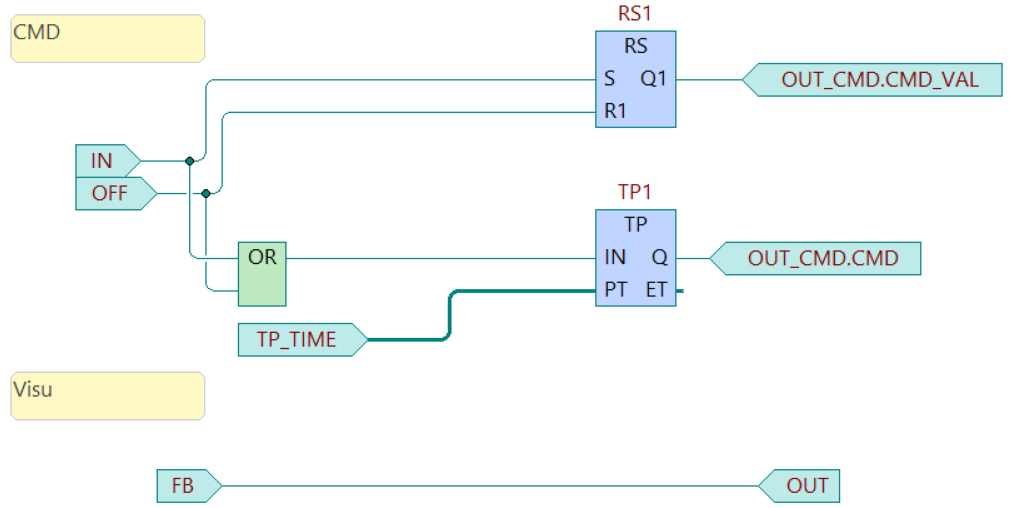
\includegraphics[scale=0.5]{obrazky/fbKNXVisuBool.png}
    \end{center}
    \caption[fbKNXVisuBool]{fbKNXVisuBool}
    \label{fig:fbKNXVisuBool}
\end{figure}
\newpage
\subsubsection{fbKNXShutters}
\begin{lstlisting}[language=ST, breaklines=true, numbers=left, numberstyle=\small, numbersep=10pt, frame=single, basicstyle=\ttfamily\small, caption={Definice funkčního bloku fbKNXShutters}, label={lst:fbKNXShutters}]
    FUNCTION_BLOCK fbKNXShutters
    VAR_INPUT
      UP           : BOOL R_EDGE; //Rolety nahoru Vizu
      DOWN         : BOOL R_EDGE; //Rolety dolu Vizu
      UP_STEP      : BOOL; //Rolety nahoru krok Vizu
      DOWN_STEP    : BOOL; //Rolety dolu krok Vizu
      FB_UP        : BOOL; //KNX Rolety Feedback nahoru
      FB_DOWN      : BOOL; //KNX Rolety Feedback dolu
    END_VAR
    VAR_OUTPUT
      OUT_CMD      : DT_CMD_BOOL; //KNX CMD
      OUT_STEP_CMD : DT_CMD_BOOL; //KNX CMD krok
      OUT_UP       : BOOL; //Visu nahoru
      OUT_DOWN     : BOOL; //Visu dolu
    END_VAR
    VAR
      TP_TIME : TIME := T#1S; //KNX CMD délka
      RS1 : RS;
      TP1 : TP;
      RS2 : RS;
    END_VAR
\end{lstlisting}

\begin{figure}[!ht]
    \begin{center}
        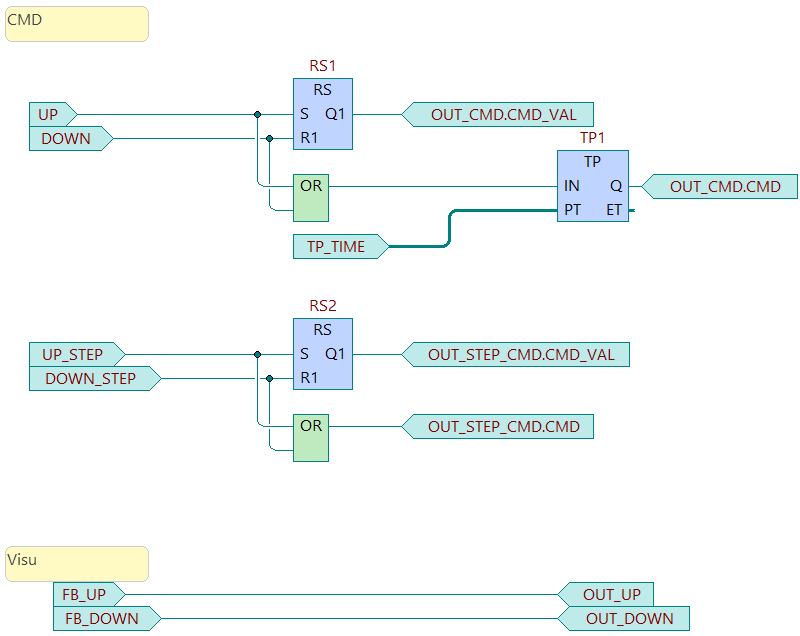
\includegraphics[scale=0.7]{obrazky/fbKNXShutters.png}
    \end{center}
    \caption[fbKNXShutters]{fbKNXShutters}
    \label{fig:fbKNXShutters}
\end{figure}
\subsubsection{fbRoomTempMod}
Na modelování teploty místnosti byl vytvořen jednoduchý matematický model, který měl za úkol zobrazit změnu v závislosti na působení topení a klimatizace. Uvažujeme, že místnost je kvádr o rozměrech specifikovaných uživatelským vstupem. Tento kvádr je naplněný vzduchem, který má určitou váhu, ze které lze vypočítat energii potřebnou ke změně teploty o 1 °C.

\begin{equation}
    V = a \cdot b \cdot c
    \label{eq:objem}
\end{equation}
\begin{equation}
    m = \rho \cdot V
    \label{eq:hmotnost}
\end{equation}
\begin{equation}
    Q = m \cdot c_p
    \label{eq:energie}
\end{equation}
\noindent\textit{Kde:}
\begin{itemize}
    \item $V$ -- objem vzduchu v místnosti [m$^3$]
    \item $a$, $b$, $c$ -- rozměry místnosti [m]
    \item $m$ -- hmotnost vzduchu v místnosti [kg]
    \item $\rho$ -- hustota vzduchu při tlaku jedné atmosféry a teplotě 20 °C - 1.204 [kg/m$^3$]
    \item $Q$ -- energie potřebná ke změně teploty o 1 stupeň teploty [J]
    \item $c_p$ -- měrná tepelná kapacita vzduchu - 1005 [J$\cdot$kg$^{-1}\cdot$K$^{-1}$] \newline
\end{itemize}
\noindent Dále uvažujeme obal kvádru (stěny, podlahu a strop) s různými tloušťkami a tepelnými vodivostmi (Fourierův zákon vedení tepla \ref{eq:tepelny_tok}). Pro zjednodušení výpočtu se předpokládá, že dveře a okna místnosti nemají rozdílný vliv oproti stěnám, tudíž tepelný tok zůstává na celé ploše strany stejný. Zároveň směr toku závisí pouze na poměru teplot na obou stranách zdi. Dále je předpoklad nulových teplot z jiných směrů. Také budeme předpokládat, že materiál bude všude stejný a to pálená cihla. 

\begin{equation}
    S = a \cdot b
    \label{eq:plocha}
\end{equation}
\begin{equation}
    \Delta T = T_{in} - T_{out}
    \label{eq:rozdil_teplot}
\end{equation}
\begin{equation}
    \phi _{Strana} = \frac{\lambda \cdot S \cdot \Delta T}{c}
    \label{eq:tepelny_tok}
\end{equation}
\noindent\textit{Kde:}
\begin{itemize}
    \item $S$ -- plocha strany [m$^2$]
    \item $a$, $b$, $c$ -- rozměry strany [m]
    \item $\Delta T$ -- rozdíl teploty na obou stranách strany [°C]
    \item $T_{in}$ -- teplota uvnitř místnosti [°C]
    \item $T_{out}$ -- teplota venku [°C]
    \item $\phi _{Strana}$ -- tepelný tok [W]
    \item $\lambda$ -- tepelná vodivost cihly - 0.4 [W$\cdot$m$^{-1}\cdot$K$^{-1}$] \newline
\end{itemize}
\noindent Další součástí simulace je topení a klimatizace, které jsou dodávány pouze jako binární signály. Pro jednoduché modelování byly vytvořeny funkce růstu (logaritmický) a poklesu (exponenciální) výkonu. Tyto funkce jsou zobrazeny na Obr. \ref{fig:simulace_funkce} Dále byly k těmto rovnicím vytvořeny korekční členy, které ovlivňují rychlost funkcí, a tedy více přiblížily chování funkcí realitě.

\begin{equation}
    f_{Růst}(t) = \frac{ln(1 + k_{Růst} \cdot t)}{ln(1 + k_{Růst} \cdot t_{MaxRůst})} \cdot y_{Max}
    \label{eq:funkce_rust}
\end{equation} 
\begin{equation}
    k_{Růst} = \frac{t_{MaxRise}}{t_{80}}
    \label{eq:k_rust}
\end{equation}
\begin{equation}
    f_{Pokles}(t) = \frac{y}{e^{k_{Pokles} \cdot t}}
    \label{eq:funkce_pokles}
\end{equation}
\begin{equation}
    k_{Pokles} = \frac{\frac{y_{max}}{\varepsilon}}{t_{MaxPokles}}
    \label{eq:k_pokles}
\end{equation}
\newpage
\noindent\textit{Kde:}
\begin{itemize}
    \item $f_{Růst}(x)$ -- funkce růstu výkonu [W]
    \item $k_{Růst}$ -- korekční člen pro pokles [-]
    \item $t$ -- čas [s]
    \item $t_{MaxRůst}$ -- maximální čas růstu výkonu [s]
    \item $y_{Max}$ -- maximální výkon [W]
    \item $t_{80}$ -- čas potřebný k dosažení 80\% výkonu [s]
    \item $f_{Pokles}(x)$ -- funkce poklesu výkonu [W]
    \item $k_{Pokles}$ -- korekční člen pro růst [-] 
    \item $y$ -- aktuální výkon [W]
    \item $\varepsilon$ -- cílová hodnota, pod kterou se výkon musí dostat [W]
    \item $t_{MaxPokles}$ -- maximální čas poklesu výkonu [s]
\end{itemize}
\begin{figure}[!ht]
    \begin{center}
        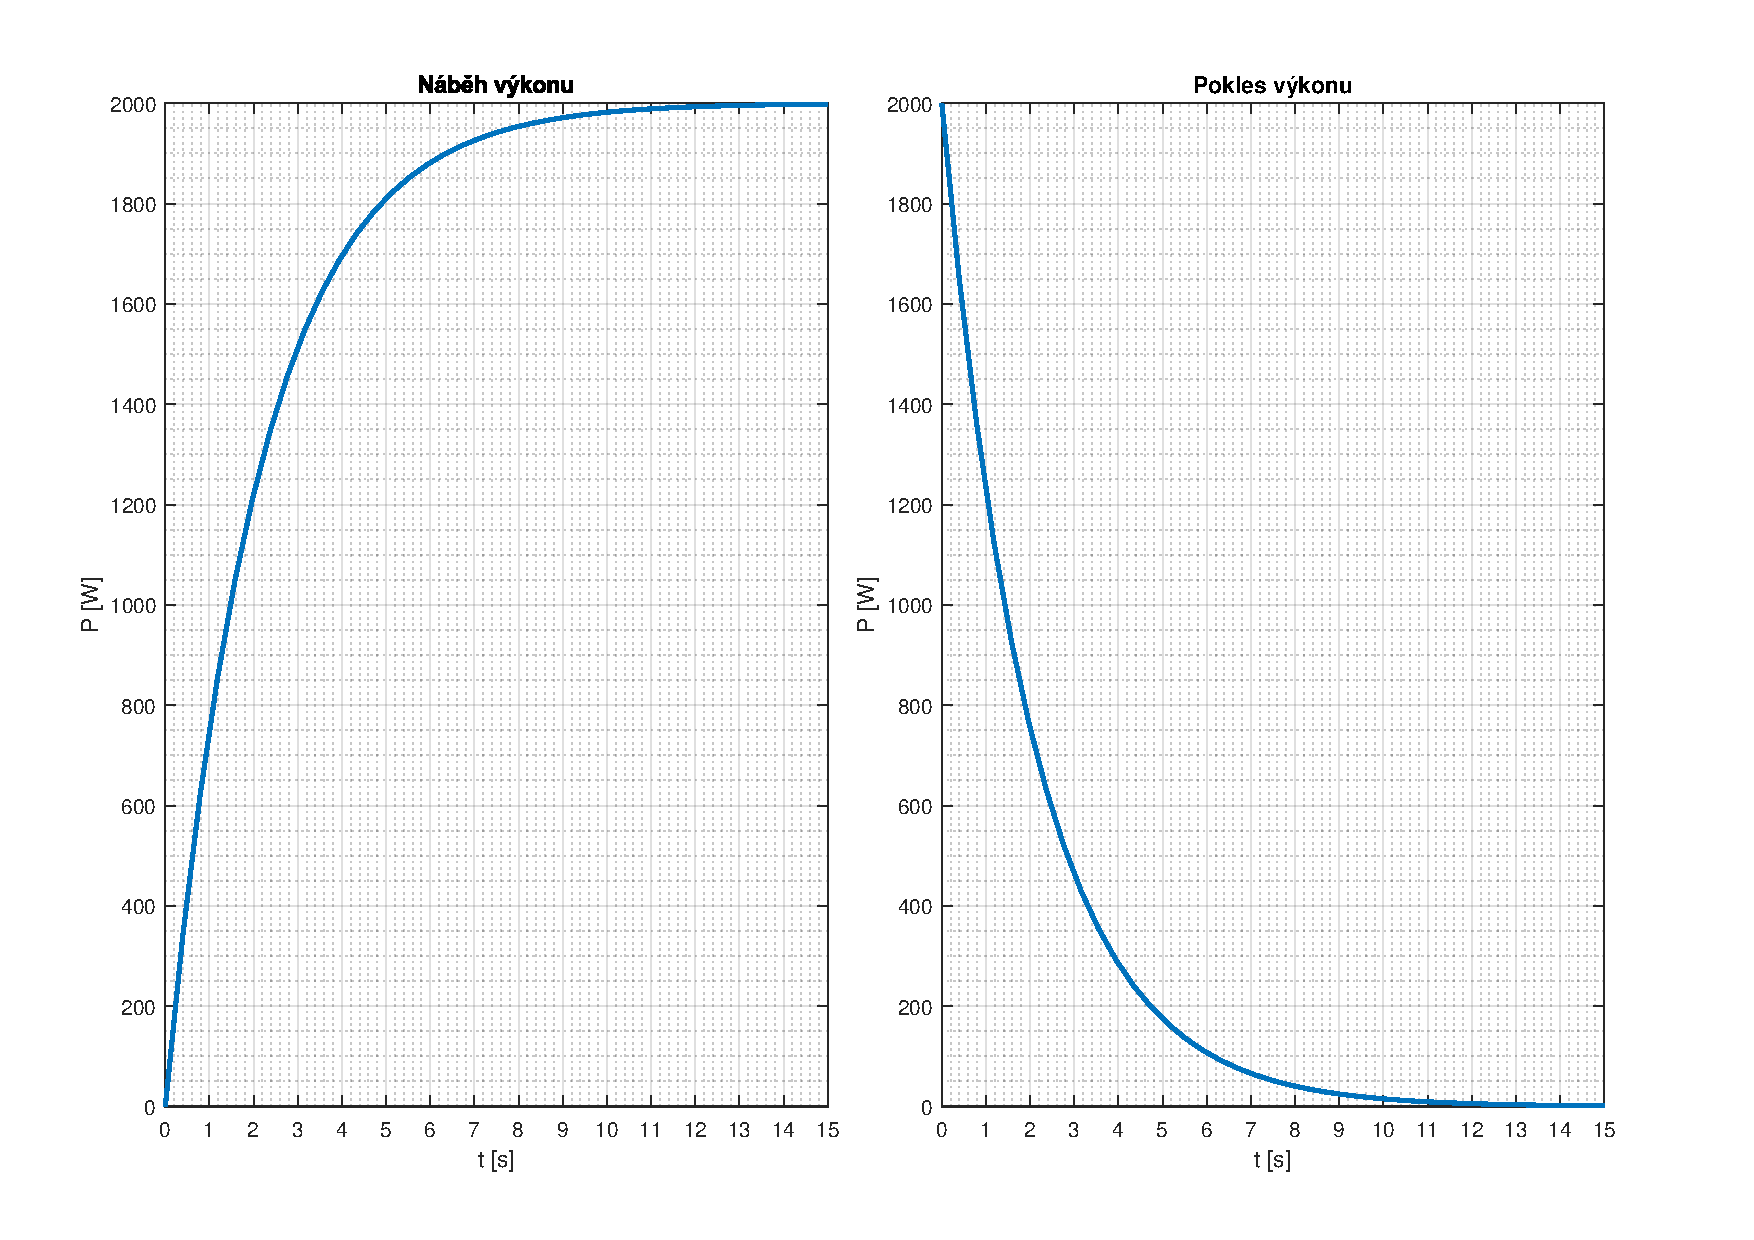
\includegraphics[scale=0.52]{obrazky/simulace_funkce.pdf}
    \end{center}
    \caption[Průběh funkcí pro simulaci]{Průběh funkcí pro simulaci}
    \label{fig:simulace_funkce}
\end{figure}
\noindent Tyto funkce bylo potřeba převést do rekurzivní podoby, aby bylo možné je implementovat do funkčního bloku.
\begin{equation}
    y_{RůstTed} = y_{RůstPred} + \frac{ln(1 + k_{Růst} \cdot \Delta t)}{ln(1 + k_{Růst} \cdot T_{Max})} \cdot (y_{Max} - y_{RůstPred}) 
    \label{eq:rust_rekurzivni}
\end{equation}
\begin{equation}
    y_{PoklesTed} = y_{PoklesPred} \cdot e^{k_{Pokles} \cdot \Delta t}
    \label{eq:pokles_rekurzivni}
\end{equation}
\noindent\textit{Kde:}
\begin{itemize}
    \item $y_{RůstTed}$ -- nový výkon [W]
    \item $y_{RůstPred}$ -- předchozí výkon [W]
    \item $k_{Růst}$ -- korekční člen pro pokles [-]
    \item $\Delta t$ -- časový krok [s]
    \item $T_{Max}$ --maximální čas růstu výkonu [s]
    \item $y_{Max}$ -- maximální výkon [W]
    \item $y_{PoklesTed}$ -- nový výkon [W]
    \item $y_{PoklesPred}$ -- předchozí výkon [W] \newline
\end{itemize}
\noindent Po vyčtení výkonu topení a klimatizace zbývá vypočítat teplotu v místnosti. Ta se získá součtem aktuální hodnoty teploty, přírůstku podílu působících toků a potřebné energie ke změně teploty. (Rov. \ref{eq:energie}). Rovnice pro celkový tepelný tok je dána jako součet tepelných toků ze stran, výkonu topení a klimatizace (působí záporně).
\begin{equation}
    T_{Aktualni} = T_{Predchozi} + \frac{\phi _{Celkovy} \cdot \Delta t}{Q}
    \label{eq:aktualni_teplota}
\end{equation}
\begin{equation}
    \phi _{Celkovy} = \sum_{i=1}^{6} \phi _{Strana_i} + \phi _{Topeni} - \phi _{Klimatizace}
    \label{eq:celkovy_tepelny_tok}
\end{equation}
\noindent\textit{Kde:}
\begin{itemize}
    \item $T_{Aktualni}$ -- aktuální teplota [°C]
    \item $T_{Predchozi}$ -- předchozí teplota [°C]
    \item $\Delta t$ -- časový krok [s]
    \item $\phi _{Celkovy}$ -- celkový tepelný tok [W]
    \item $\phi _{Strana_i}$ -- tepelný tok ze strany \textit{i} [W]
    \item $\phi _{Topeni}$ -- tepelný tok z topení [W]
    \item $\phi _{Klimatizace}$ -- tepelný tok z klimatizace [W] \newline
\end{itemize}

\noindent Průběh teploty v místnosti je zobrazen na Obr. \ref{fig:simulace_teplota}, kde je demonstrováno chování při běhu topení a klimatizace v horním grafu. Ve spodní části grafu je zase zobrazeno chování teploty bez působení topení a klimatizace. Teplota okolí je v tomto případě nastavená na 21 °C. Z průběhu lze vypozorovat, že se teplota ustálí na teplotu okolí a tudíž, lze považovat model za korektní.
\newpage
\begin{figure}[!ht]
    \begin{center}
        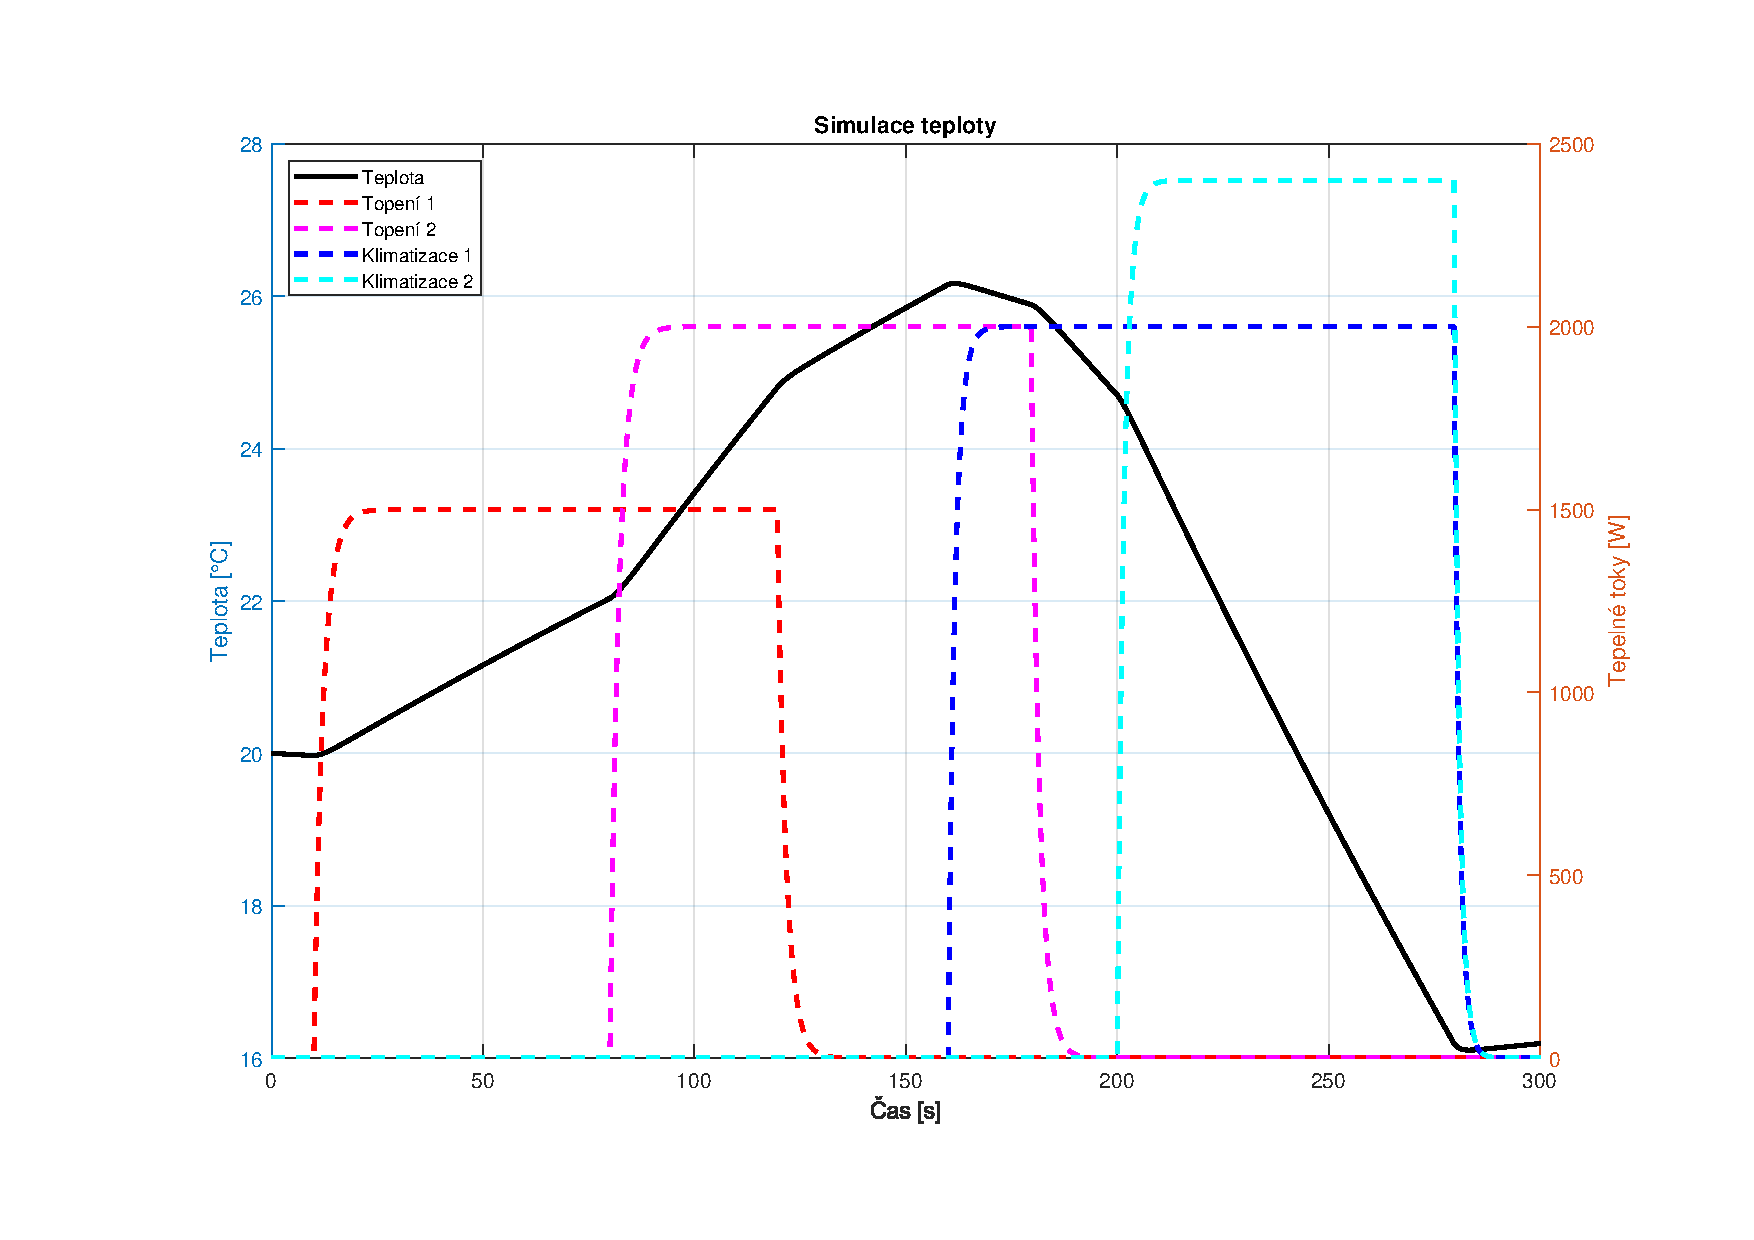
\includegraphics[scale=0.52]{obrazky/simulace_teploty_kuchyne.pdf}
    \end{center}
    \caption[Simulace teploty v místnosti]{Simulace teploty v místnosti}
    \label{fig:simulace_teplota}
\end{figure}

\noindent Tento funkční blok byl použit pro simulaci teploty v obývacím pokoji, kuchyni. Definice tohoto funkčního bloku je zobrazena kvůli své velikosti v příloze \ref{apend:fbRoomTempMod}. Pro venkovní teplotu byl použit signál, který byl napojen na teploměr na panelu. V případě koupelny byla teplota simulována jako sinusoida v rozmezí 18-22 °C s periodou 3 minuty. Tento způsob byl zvolen kvůli absenci teploměru a akčního členu pro řízení teploty. 

\subsubsection{funkční bloky jednotlivých místností}
\label{subsection:fb_mistnosti}
Funkční bloky jednotlivých místností se skládají z výše uvedených funkcí, které byly poskládány v závislosti na požadavcích jednotlivých místností - viz Obr. \ref{fig:Vzheled panelu}. Všechny funkční bloky mají definici vypsanou v přílohách dokumentu:
\begin{itemize}
    \item \textbf{fbBath} - V příloze \ref{apend:fbBath}
    \item \textbf{fbKitch} - V příloze \ref{apend:fbKitch}
    \item \textbf{fbLivRoom} - V příloze \ref{apend:fbLivRoom}
    \item \textbf{fbOutz} - V příloze \ref{apend:fbOutz}
\end{itemize}
\subsection{Komunikace KNX/IP}
Důležitou součástí ovládání instalace je komunikace s KNX/IP, která byla realizována pomocí knihovny KNXlib \cite{KNXlib}. Obsahem této knihovny jsou dva funkční bloky určené ke komunikaci:
\begin{itemize}
    \item \textbf{fbKnxIpBaos} - Funkční blok pro komunikaci s KNX/IP BAOS 772 v režimu TCP master
    \item  \textbf{fbKnxIpBaosBin} - Funkční blok pro komunikaci s KNX/IP BAOS 772/774 skrze binární protokol v režimu TCP Master \newline
\end{itemize}
Dále tato knihovna obsahuje datové struktury, které obsahují definice jednotlicých datapointů, které jsou potřeba pro komunikaci mezi PLC a KNX/IP Baos 774:
\begin{table}[h]
    \caption[Definice KNX datapointů v PLC]{Definice KNX datapointů v PLC}
        \small
            \centering
            \begin{tabular}{|c|c|c|}
                \hline
                Typ objektu KNX & Datový typ PLC & Popis  \\
                \hline\hline
                DPT 01 & T\_KNX\_OBJECT\_DPT1 & Binární signál -- 1 Bit \\
                \hline
                DPT 02 & T\_KNX\_OBJECT\_DPT2 & Binární signál s kontrolou (Priorita) -- 2 Bity \\
                \hline
                DPT 03 & T\_KNX\_OBJECT\_DPT3 & Stmívání nahoru/dolů -- 4 Bit \\
                \hline
                DPT 04 & T\_KNX\_OBJECT\_DPT4 & Znak -- 1 bajt \\
                \hline
                DPT 05 & T\_KNX\_OBJECT\_DPT5 & Škálování -- 1 bajt (8 Bitová hodnota) \\
                \hline
                DPT 06 & T\_KNX\_OBJECT\_DPT6 & Hodnota se znaménkem -- 1 bajt \\
                \hline
                DPT 07 & T\_KNX\_OBJECT\_DPT7 & Hodnota bez znaménka -- 2 bajty \\
                \hline
                DPT 08 & T\_KNX\_OBJECT\_DPT8 & Hodnota se znaménkem -- 2 bajty \\
                \hline
                DPT 09 & T\_KNX\_OBJECT\_DPT9 & Hodnota s desetinnou čárkou -- 2 bajty\\
                \hline
                DPT 10 & T\_KNX\_OBJECT\_DPT10 & Čas -- 3 bajty \\
                \hline
                DPT 11 & T\_KNX\_OBJECT\_DPT11 & Datum -- 3 bajty \\
                \hline
                DPT 12 & T\_KNX\_OBJECT\_DPT12 & Hodnota bez znaménka -- 4 bajty \\
                \hline
                DPT 13 & T\_KNX\_OBJECT\_DPT13 & Hodnota se znaménkem -- 4 bajty \\
                \hline
                DPT 14 & T\_KNX\_OBJECT\_DPT14 & Hodnota s desetinnou čárkou -- 4 bajty \\
                \hline
                DPT 15 & T\_KNX\_OBJECT\_DPT15 & Přístupová data -- 4 bajty \\
                \hline
                DPT 16 & T\_KNX\_OBJECT\_DPT16 & Řetězec znaků -- 14 bajty \\
                \hline
                DPT 17 & T\_KNX\_OBJECT\_DPT17 & Scéna -- 1 bajt \\
                \hline
                DPT 18 & T\_KNX\_OBJECT\_DPT18 & Kontroler scén -- 1 bajt \\
                \hline
                DPT unknown & T\_KNX\_OBJECT\_RAW & Max. 14 bajtů, Data jako pole, byte-by-byte \\
                \hline
            \end{tabular}
\end{table}
\subsubsection{Realizace komunikace KNX/IP}
Pro realizaci v tomto případě bylo potřeba kromě přidání knihovny a vytvoření programu ještě i nastavit ethernet port. V tomto případě byl do \textit{ETH2} přidán obecný kanál \textit{UNI1}, který bylo potřeba nastavit jako TCP Server. Dále je pak nutné vytvořit několik proměnných dle tabulky datapointů \ref{tab:Datapointy pro komunikaci KNX IP BAOS 774 s PLC}, získat jejich adresy a poté je vložit do pole.

Dalším krokem je nastavení funkčního bloku \textit{fbKnxIpBaosBin}. Nejprve se nastaví číslo prvního a posledního datapointu, který má funkční blok zpracovat, poté se nastaví použitý ethernet port a IP adresa KNX/IP BAOS 774 instalace. Nakonec se předá do portu \textit{knxList} námi definované pole s adresami. Po tomto kroku je už možné pracovat s proměnnými a vytvoření ovládací logiku.

V případě této práce se používají pouze 3 druhy datapointů a to:
\begin{itemize}
    \item \textbf{DPT 1} - ovládání a indikace binárního signálu
    \item \textbf{DPT 9} - hodnota teploty z teploměru
    \item \textbf{DPT 18} - ovládání scény \newline
\end{itemize}
Níže je uvedena ukázka realizace komunikace, která vyplývá z implementace uvedené v příloze \ref{apend:KNXComm}:
\begin{lstlisting}[language=ST, breaklines=true, numbers=left, numberstyle=\small, numbersep=10pt, frame=single, basicstyle=\ttfamily\small, caption={Implementace komunikace KNX/IP}, label={lst:komunikace_knx}]
PROGRAM prgKNXComm
  VAR
    init : BOOL;
    knx  : fbKnxIpBaosBin;
    knxObjectList    : ARRAY[1..4] OF UDINT; // pole adres
    datapoint1      : T_KNX_OBJECT_DPT1;     // SV1_FB
    datapoint2      : T_KNX_OBJECT_DPT1;     // SV1_CMD
    datapoint3      : T_KNX_OBJECT_DPT18;    // scéna
    datapoint4      : T_KNX_OBJECT_DPT9;     // teplota
  END_VAR

IF NOT init THEN // Pole adres
  knxObjectList[1]  := PTR_TO_UDINT( ADR(datapoint1));
  knxObjectList[2]  := PTR_TO_UDINT( ADR(datapoint2));
  knxObjectList[3]  := PTR_TO_UDINT( ADR(datapoint3));
  knxObjectList[4]  := PTR_TO_UDINT( ADR(datapoint4));
  init := TRUE;
END_IF

knx( firstKnxObject := 1,
     lastKnxObject := 4,
     ethCode := ETH2_uni2,
     knxIP := STRING_TO_IPADR('192.168.xxx.xxx'),
     knxList := void( knxObjectList));
\end{lstlisting}
\begin{lstlisting}[language=ST, breaklines=true, firstnumber=25, numbers=left, numberstyle=\small, numbersep=10pt, frame=single, basicstyle=\ttfamily\small]

SV1_FB := datapoint1.value; // Feedback
IF SV1_CMD THEN datapoint2.value := SV1_CMD.CMD_VAL; // CMD

IF SCENE THEN // scéna
  datapoint3.control := TRUE;
  datapoint3.scene   := 5;
END_IF

KNX_TEMPER := datapoint4.value;// Posílání teploty
END_PROGRAM
\end{lstlisting}
\subsection{Komunikace MQTT}
\label{subsection:MQTT}
Tato sekce je zaměřená na realizaci komunikace skrze protokol MQTT, který je navržen jako lehký přenos zpráv mezi zařízeními a aplikacemi. Jeho cílovou skupinou jsou zařízení s malou kódovou stopou a minimální šířkou pásma sítě. \cite{MQTT}

\subsubsection{Protokol}
Základními myšlenkami protokolu MQTT je posílání zpráv mezi vydavatelem (publisher) a odběratelem(client) skrze zprostředkovatele (broker). Tento broker zajišťuje, že zprávy jsou doručeny správným odběratelům. Vydavatel a odběratel nemusí být navzájem známi a komunikují pouze skrze brokera. \cite{MQTT}

Tento druh komunikace je realizován pomocí packetů (balíků dat) posílaných mezi zařízeními. Jednotlivé datové balíky jsou tvořen třemi částmi \cite{MQTTEsentials}:
\begin{itemize}
    \item \textbf{Fixní hlavičku} - obsahuje informace o typu packetu, příznaky a velikost zbylé části packetu 
    \item \textbf{Volitelnou hlavičku} - obsahuje dynamické informace o packetu
    \item \textbf{Datový obsah} - obsahuje data, která se posílají mezi zařízeními \newline
\end{itemize}
Zprávy se poté posílají na určité téma (topic), které je definováno jako hierarchická struktura. Tato struktura je tvořena jednotlivými úrovněmi oddělenými lomítkem. V případě této práce je dobrým příkladem téma \textit{plc/Connect/Publisher}, kde:
\begin{itemize}
    \item \textbf{plc} - označuje zařízení, které zprávu odesílá
    \item \textbf{Connect} - která část systému zprávu odesílá
    \item \textbf{Publisher} - bližší rozlišení \newline
\end{itemize}
Dálší část je text samotné zprávy, která je odeslána na dané téma. Tato zpráva může mít libovolnou strukturu i velikost(maximálně 256 MB). Tělem zprávy je text ve formátu JSON, který se lze pochopit jako hierarchická struktura dat. Vertikálně je struktura rozdělena do úrovní pomocí vnořených objektů a polí. Horizontálně je struktura členěna do jednotlivých klíč:hodnota párů na jedné úrovni, kde každý klíč reprezentuje konkrétní parametr. Příkladem takové zprávy je:
\begin{lstlisting}[language=JSON, breaklines=true, numbers=left, numberstyle=\small, numbersep=10pt, frame=single, basicstyle=\ttfamily\small, caption={Příklad zprávy v JSON}, label={lst:json}]
{
    "device": "plc",
    "location": {
        "room": "kitchen",
        "floor": 1
    },
    "sensors": {
        "temperature": {
            "value": 22.5,
            "unit": "C"
        },
        "humidity": {
            "value": 45,
            "unit": "%"
        }
    },
    "status": "online",
    "timestamp": "2024-06-01T12:34:56Z"
}
\end{lstlisting}

\noindent Součástí zprávy je i kvalita služeb \textit{QoS} (Quality of Service), která určuje úroveň spolehlivosti doručení zprávy. Tato úroveň je nastavena na 0 (doručení maximálně jednou bez záruky), 1(doručená alespoň jednou) nebo 2(doručená přesně jednou s potvrzením příjemce) \cite{MQTTEsentials}. V případě této práce byla zvolena úroveň QoS 1, která je dostatečná pro většinu aplikací a poskytuje dobrou rovnováhu mezi spolehlivostí a výkonem. 

Poslední součástí zprávy je \textit{Last Will and Testament} (LWT), což je zpráva, která je odeslána brokerem v případě, že se zařízení odpojí bez předchozího oznámení. Tato zpráva může být užitečná pro monitorování stavu zařízení a detekci výpadků \cite{MQTTEssentials}.

\subsubsection{MQTTlib}
Pro realizaci komunikace mezi PLC a Home Assistantem byla použita knihovna MQTTlib, která obsahuje funkční bloky pro nastolení komunikace - \textit{fbMQTTPublisher}, \textit{fbMQTTSubscriber}. \cite{MQTTlib}

Prvním krokem pro realizaci komunikace je nastavení ethernet portu, který bude použit pro komunikaci. V případě této práce byl použit stejný port jako pro KNX/IP komunikaci (\textit{ETH2}). Na tomto portu byly vytvořeny dva obecné kanály \textit{UNI0} a \textit{UNI1}, které byly nastaveny jako TCP clienty s šíkou pásma 512 bytů. Počet kanálu závisí na počtu nastolených spojení. Pro jednoduchost se jedná o jedno spojení pro publikování a jedno pro odběr zpráv. 

Dalším krokem je nastavení funkčních bloků. V obou případech je nastavení obdobné. Nejprve se nastaví kanál na kterém bude komunikace probíhat - IP adresa brokeru, port brokeru, lokální port, časový interval pro kontrolu spojení a délku nečinosti. Dále se nastaví parametry komunikace a poslední vůle:
\begin{itemize}
    \item \textbf{clientID\_auto} - automatické generování identifikátoru klienta
    \item \textbf{clientID} - identifikátor klienta
    \item \textbf{loginName} - uživatelské jméno pro připojení k brokeru
    \item \textbf{loginPass} - heslo pro připojení k brokeru
    \item \textbf{retain} - určuje zda má být zpráva uchována na brokeru
    \item \textbf{QoS} - určuje úroveň kvality služeb
    \item \textbf{cleanSession} - určuje zda má broker uložit stav relace po výpadku
    \item \textbf{topic} - téma komunikace
    \item \textbf{mess} - zpráva komunikace
    \item \textbf{flag} - určuje zda má být poslední vůle odeslána v případě odpojení klienta bez předchozího oznámení \newline
\end{itemize}

Po nastavení funkčních bloků je potřeba definovat proměnné na uchovávání zpráv. Maximální délka zprávy je 256 znaků pro oba funkční bloky. Níže je uveden příklad nastavení komunikace pro publikování zprávy:
\begin{lstlisting}[language=ST, breaklines=true, numbers=left, numberstyle=\small, numbersep=10pt, frame=single, basicstyle=\ttfamily\small, caption={Příklad nastavení komunikace pro publikování zprávy}, label={lst:publikace}]
PROGRAM prgMQTTPub
    VAR
        mqttPub : fbMQTTPublisher;

        brokerIPaddr      : STRING := '192.168.xxx.xxx'; // IP adresa brokeru
        brokerPort        : UINT := 1883; // Port brokeru
        localPort         : UINT := 60000; // Lokalni port
        keepAlive         : BOOL  := TRUE; // Udrzeni spojeni po vypadku
        keepAliveInterval : TIME  := T#60s; // Konec spojeni bez dat
        pingInterval      : TIME  := T#10s; // Kontrola spojeni
\end{lstlisting}
\begin{lstlisting}[language=ST, breaklines=true, firstnumber=11, numbers=left, numberstyle=\small, numbersep=10pt, frame=single, basicstyle=\ttfamily\small]
        connTimeOut       : TIME  := T#5s; // Maximalni delka odezvy

        pubComParam   : T_MQTT_COM_PUB_PARAM := (
        pRetain := TRUE, // Uchovani zpravy na brokeru
        qos     := 1, // Kvalita sluzeb
        dup     := FALSE, // Opakovani zpravy
        clean   := FALSE // Uchovani stavu relace
        );

        willParamPub  : T_MQTT_COM_WILL_PARAM := (
        wRetain := FALSE, // Uchovani posledni vule na brokeru
        topic   := 'plc/Connect/Publisher', // Tema poslední vule
        mess    := 'Disconnected', // Zprava posledni vule
        flag    := TRUE, // Odeslani posledni vule
        qos     := 1 // Kvalita sluzeb
        );

        jsonPayload : STRING[255]; // Zprava
        topic      : STRING[80] := 'plc/test'; // Tema
    END_VAR

jsonPayload := CONCAT(
    '{',"test",'}'
);
mqttPub(
    chanCode          := ETH2_uni1, // Fyzicky kanal
    brokerIP          := STRING_TO_IPADR(brokerIPaddr),
    brokerPort        := brokerPort,
    localPort         := localPort,
    connect           := TRUE, // Pripojit k brokeru
    keepAlive         := keepAlive,
    keepAliveInterval := keepAliveInterval,
    pingInterval      := pingInterval,
    connTimeOut       := connTimeOut,
    clientId_auto     := FALSE, // Automaticke generovani ID
    clientId          := 'TEST_PUB', // ID klienta
    comParam          := pubComParam, // Parametry komunikace
    willParam         := willParamPub, // Parametry posledni vule
    topicTxt          := topic, // Tema
\end{lstlisting}
\pagebreak
\begin{lstlisting}[language=ST, breaklines=true, firstnumber=50, numbers=left, numberstyle=\small, numbersep=10pt, frame=single, basicstyle=\ttfamily\small]
    dataTxt           := jsonPayload, // Zprava
    sendCom           := TRUE // Odeslani zpravy
);
END_PROGRAM
\end{lstlisting}

Implementace použitá v této práci je uvedena v příloze \ref{apend:MQTTComm}. Jedná se o nastavení komunikace pro komunikaci s Home Assistantem, který přijímá hodnoty teplot místností a odesílá příkaz pro celkové vypnutí instalace. 
\subsection{Vizualizace}
V této sekci je popsána tvorba vizualizace panelu pomocí integrovaného webového serveru. Nastavení a realizace webového serveru je realizována pomocí integrovaného nástroje WebMaker. Tento nástroj je popsán v dokumentaci \cite{WebMaker}.

Prvním krokem je vytvoření struktury projektu. V tomto případě to bude 5 stránek ve formátu .XML zasazených do webové struktury: \newline

\dirtree{%
.1 /Vizualizace.
.2 Prehled - PAGE1.xml.
.2 Veranda - PAGE2.xml.
.2 Kuchyn - PAGE3.xml.
.2 Koupelna - PAGE4.xml.
.2 Obyvaci\_pokoj - PAGE5.xml. 
}
\vspace{0.3cm}
Druhým krokem bylo importování sady ikon, které byly použity jako vícerozměrné obrázky napojené na výstupy funkčních bloků uvedených v podkapitole \ref{subsection:fb_mistnosti}. Tyto ikony byly získány na stránce Flaticon \cite{Flaticon}, která poskytuje vektorové ikony na projekty zdarma s možností úpravy. 


\begin{figure}[!ht]
    \begin{center}
        
\includegraphics[scale=0.6]{obrazky/Ikonky.png}
    \end{center}
    \caption[Ikony použité pro vizualizaci]{Ikony použité pro vizualizaci}
    \label{fig:ikony}
\end{figure}

Dále se musely vytvořit ovládací tlačítka jednotlivých objektů. Tato tlačítka byla také vytvořena jako vícerozměrné obrázky, které byly napojeny na vstupy funkčních bloků. Pro zobrazování teplot v jednotlivých místnostech byla použita zadávací pole s parametrem \textit{Read only}. 
Výsledná vizualizace je uvedena v příloze \ref{apend:webmaker}. Vzhled byl zvolen minimalistický a funkční s ohledem na viditelnost a přehlednost. Černé pozadí zdůrazňuje kontrast ikon a textu. Dalším důvodem byla ochrana zraku při ovládání v noci.
\chapter{Open-source platformy}
Tato kapitola se zaměřuje na možnost vizualizace a ovládní domácí automatizace pomocí open-source technologií (software s otevřeným kódem), které je možné využít v případě nedostatku financí nebo pro uživatele, kteří chtějí mít plnou kontrolu nad svým systémem. V případě tohoto řešení byl vybrán přístup pomocí kontejnerizace, který umožňuje snadné nasazení a škálování aplikací, ale také snadné zálohování a migraci v případě poruch.

\section{Raspberry Pi 5}
Jedná se o jednodeskový počítač, který je určen pro široké spektrum aplikací od IoT, rozpoznávání obrazu, strojového učení, robotiky až po multimediální aplikace. Mezi hlavní výhody patří nízká cena, malé provozní náklady, možná modularita přes GPIO piny, PCI expres a USB porty a velké množství tzv. HAT modulů, které jsou určeny pro rozšíření funkcí. \cite{Raspberry Pi 5}.

Pro tuto aplikaci bylo zvoleno Raspberry Pi 5 s 16 GB RAM, pamětí 256 GB a operačním systémem Raspberry Pi OS, který je stavěn na Linuxové distribuci Debianu. Hlavním důvodem výběru byla nízká cena, ale i jednoduchá dostupnost pro případného zájemce o domácí automatizaci, který by si chtěl systém ovládání a vizualizace vytvořit sám.

Jediným závažnějším problémem tohoto zařízení je degradace paměťové karty, na které je nahrán operační systém. Tento problém je způsoben častým zápisem, který postupně snižuje životnost, rychlost a velikost paměti. V krajních případech může dojít i k úplnému zničení a ztrátě dat. K předcházení tohoto problému se historicky používala technika \textit{wear leveling} - rozložení zápisu na celou paměťovou kartu, aby se snížil počet zápisů na jednotlivé buňky \cite{wear leveling}. Teď už je možné použít M.2 NVMe SSD disk, který je připojen přes PCI expres a je mnohem rychlejší než paměťová karta. Tento disk je možné použít i jako bootovací disk, což zamezí problémům s bootováním a ztrátou dat. Další možností, jak zpomalit tuto degradaci, je připojení USB flash disku. Flash disk dokáže zamezit opotřebování paměti díky přenesení souborů s vyšší frekvencí zápisu - v tomto případě databáze, nicméně rychlost zápisu se tímto sníží.
\begin{figure}[!ht]
    \begin{center}
        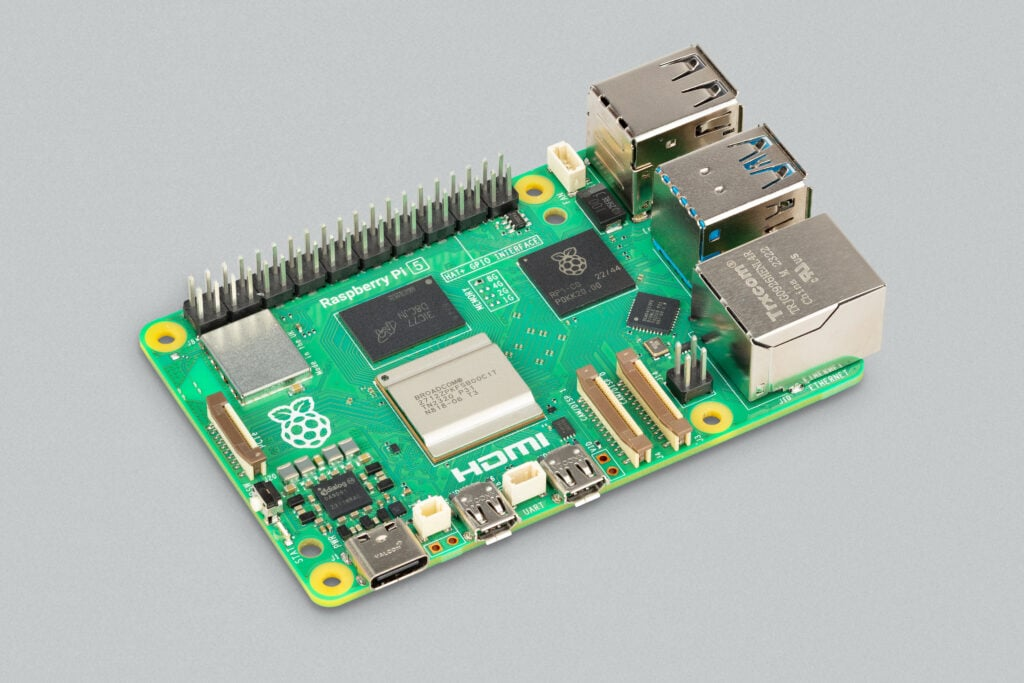
\includegraphics[scale=0.30]{obrazky/RaspberryPi5.jpg}
    \end{center}
    \caption[Raspberry Pi5~\cite{Raspberry Pi 5}]{Raspberry Pi5~\cite{Raspberry Pi 5}}
    \label{fig:RaspberryPi}
\end{figure}
\newpage
Alternativou k Raspberry Pi 5 mohou být LattePanda, ASUS NUC a podobné mikropočítače, které mají vyšší výkon, větší možnost výběru operačního systému (dostatečný výkon na Windows) a robustnost. Tyto výhody jsou kompenzovány vyšší pořizovací cenou, spotřebou a velikostí.
\section{Docker Compose}
Docker Compose je nástroj pro definici a správu více kontejnerových aplikací. Umožňuje uživatelům definovat aplikaci pomocí \textit{YAML} souboru, které obsahují informace o kontejnerových službách, sítích a úložištích. \cite{Docker Compose}

Instalace Docker Compose je jednoduchá a rozepsaná na oficiálních stránkách Dockeru. Obsahuje pouze tři kroky, které jsou již připraveny pro kopírování do terminálu. \cite{DockerInstallationForDebian}

\subsection{Kontejnerizace}
Kontejnerizace je způsob virtualizace aplikací založený na linuxové technologii LXC (Linux Containers), která umožňuje spouštět aplikace v izolovaném prostředí se zárukou jejich funkčnosti v různých systémech. Tento přístup je výhodný pro nasazení aplikací s různými závislostmi a konfiguracemi a umožňuje jejich snadné nasazení i škálování. Na rozdíl od tradičních virtuálních strojů poskytuje kontejnerizace kompletní běhové prostředí s menšími nároky na výkon a paměť, protože nevyžaduje samostatný kernel ani simulaci veškerého hardwaru. \cite{ContainerAndVirtualization}
V případě této práce byl navrhnut Docker Stack, který je složen z několika kontejnerů, které spolu komunikují a vytváří tak komplexní systém na ovládání a vizualizaci domácí automatizace. Vzhled tohoto stacku i s komunikacemi je zobrazen na Obr. \ref{fig:DockerStack}.
\begin{figure}[!ht]
    \begin{center}
        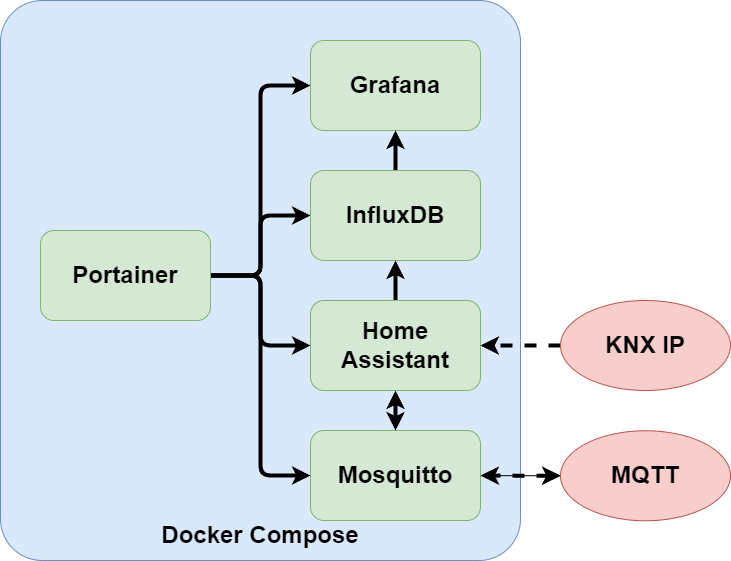
\includegraphics[scale=0.30]{obrazky/stack.png}
    \end{center}
    \caption[Docker Stack]{Docker Stack }
    \label{fig:DockerStack}
\end{figure}
\subsection{Tvorba YAML souboru}
YAML soubor je textový soubor, který obsahuje definici kontejnerů a jejich konfigurací. Je napsán v jazyce YAML (YAML Ain't Markup Language), což je formát pro serializaci dat \cite{YAML}. Níže je příklad vzhledu YAML souboru (Výpis \ref{lst:dockeryaml}), který by měl pomoci ke snadnému pochopení struktury a syntaxe \cite{ComposeYamlExample}.

Dále pak může YAML soubor obsahovat i enviromentální proměnné, které se používají k nastavení kontejneru. Tyto proměnné mohou být obsaženy v souboru .env, který se používá k uchovávání citlivých informací, jako jsou například hesla a API klíče. Tento soubor je načítán při spuštění kontejneru. \cite{ENV}
\begin{lstlisting}[language=YAML, breaklines=true, numbers=left, numberstyle=\small, numbersep=10pt, frame=single, basicstyle=\ttfamily\small, caption=YAML soubor, label=lst:dockeryaml]
version: "3" # Verze Docker Compose
services: # Sluzby
    name_of_service: # Jmeno sluzby
        image: name_of_image:latest # Jmeno image
        container_name: name_of_container # Jmeno kontejneru
        networks: # Site
            - name_of_network # Jmeno site na ktere pobezi kontejner
        depends_on: # Zavislosti
            - name_of_service # Jmeno kontejneru na kterem zavisi
\end{lstlisting}
\pagebreak
\begin{lstlisting}[language=YAML, breaklines=true, numbers=left, firstnumber=10, numberstyle=\small, numbersep=10pt, frame=single, basicstyle=\ttfamily\small]
        environment: # Promenne prostredi
            - PUID=1000 # ID uzivatele, ktery bude mit pristup k souborum
            - PGID=1000 # ID skupiny, ktera bude mit pristup k souborum
            - TZ=Europe/Prague # Casove pasmo
            - WEBUI_PORT=1234 # Port na kterem pobezi webove rozhrani 
            - DOCKER_MODS="linuxserver/mods:universal" # Docker modifikace
        volumes: # Slozky, ktere budou pripojeny do kontejneru
            - "/path/on/host:/path/in/container" # Cesta k souborum
        ports: # Porty pro pripojeni k hostitelske site
            - "host_port:container_port"
        deploy: # Nasazeni kontejneru
            resources:
                limits:
                    memory: 512m # Maximalni pamet
                    cpus: "1" # Maximalni CPU
                reservations:
                    memory: 256m # Minimalni pamet
                    cpus: "0.5" # Minimalni CPU
        restart: always # Restart kontejneru pri padu
        labels: # Metada
            - "com.docker.compose.project=project_name" # Nazev projektu
            - "com.docker.compose.service=service_name" # Nazev sluzby
            - "com.docker.compose.version=1.0" # Verze sluzby
\end{lstlisting}
\noindent Celková implementace a je zobrazena v příloze~\ref{apend:dockeryaml}.
\subsection{Portainer}
Jedná se o open-source kontejner, který slouží jako webové rozhraní pro správu Dockeru. Umožňuje uživatelům spravovat kontejnery, image (obrazy – šablony pro vytváření kontejnerů), 
stohy (stohy – skupiny kontejnerů, které spolu komunikují), sítě, uložiště, čtení logů, sledování výkonu, správa portů a další funkce. Jednou z předních výhod je jednoduchost použití; kromě rozhraní (Obr.~\ref{fig:portainer}) je i propojení s Docker Hubem, což je veřejná knihovna kontejnerů. \cite{Portainer} 
\begin{figure}[!ht]
  \begin{center}
  \includegraphics[scale=0.39]{obrazky/portainer.png}
  \end{center}
  \caption[Portainer Stack]{Portainer Stack}
  \label{fig:portainer}
\end{figure}
\pagebreak
\section{Mosquitto}
Mosquitto je open-source broker společnosti Eclipse pro protokol MQTT (Message Queuing Telemetry Transport – více v podkapitole \ref{subsection:MQTT}). Zajišťuje komunikaci mezi vydavatelem a odběratelem v závislosti na oprávněních a kvalitě služeb (\textit{QoS}). Jednou z výhod tohoto brokeru je jednoduchost implementace a nízké nároky na výkon. Dále umožňuje šifrování pomocí \textit{TLS}, které zajišťuje bezpečnost přenosu dat, podporuje cloudové služby a různé platformy. K dispozici je také knihovna pro jazyk \textit{C}, která implementuje celý protokol. \cite{Mosquitto}

V této práci byl použit kontejner pro komunikaci mezi Home Assistantem a PLC. Tento kontejner byl nastaven na porty 1883 a 9001. Port 1883 je standardní port pro MQTT protokol a používá se ke komunikaci mezi brokerem a PLC. Port 9001 je určen pro WebSocket, což je protokol pro komunikaci mezi webovými aplikacemi a servery. Proto byl použit pro komunikaci mezi Home Assistantem a Mosquittem.

Různé porty v brokeru nemají vliv na funkčnost komunikace, protože broker je schopen komunikovat na více portech současně. To znamená, že broker může přijímat zprávy na jednom portu a odesílat je skrze jiný port, pokud je použito správné téma (\textit{topic}). Dále nezáleží na pořadí příchodu zpráv, protože broker je zpracovává sekvenčně – v pořadí, v jakém přišly.
\section{Home Assistant}
Home Assistant je open-source platforma pro domácí automatizaci, která v posledních letech získala velkou popularitu. Umožňuje propojení více zařízení různých výrobců, databází a protokolů do jednoho systému. Dále pak umožňuje uživatelům monitorovat spotřebu, vytvářet vlastní vizualizace, automatizace a scénáře pro ovládání zařízení. Tato platforma je dostupná v kontejnerové podobě, jako operační systém nebo jako virtuální stroj. \cite{Home Assistant}

Jednotlivá zařízení lze implementovat prostřednictvím tzv. integrací, které jsou buď předinstalované v Home Assistantu, nebo dostupné jako pluginy. Portfolio zařízení i funkcí lze dále rozšířit pomocí komponent vyvíjených komunitou, které jsou dostupné prostřednictvím pluginu \textit{HACS} (Home Assistant Community Store). \cite{HACS}

Přidání KNX zařízení do Home Assistantu je možné pomocí integrace \textit{KNX}, která umožňuje implementaci skrze YAML soubor, ale také pomocí webového rozhraní. V této práci byla zvolena druhá možnost, která je jednodušší a rychlejší. Prvním krokem byl výběr a nastavení spojení s KNX - \textit{routing}, \textbf{\textit{tunneling}} (více v podkapitole \ref{KNXnet/IP}). Dalším krokem bylo vložení projektu instalace vygenerovaného pomocí \textit{ETS}, který obsahoval všechny potřebné informace o zařízeních a jejich adresách. Posledním krokem byla tvorba jednotlivých entit, které se vkládaly pomocí webového rozhraní - výběr typu entity, její název a adres jednotlivých funkcí. Například pro světlo bylo potřeba nastavit adresu pro ovládání, adresu pro stav, adresu pro jas a adresy pro nastavení barev. Tyto adresy se pak vybíraly ze seznamu, který se vygeneroval při vložení projektu. Existuje také možnost použít i vlastní adresy, které v projektu dosud neexistují.

Pro komunikaci mezi Home Assistantem a PLC byla použita integrace \textit{MQTT}, která se nastavila pomocí webového rozhraní a konfiguračního souboru YAML (Příloha \ref{apend:configyaml}). Webové rozhraní slouží k nastavení IP adresy, portu, uživatelského jména a hesla pro připojení k brokeru. YAML soubor slouží pro vytvoření jednotlivých entit.

Po vytvoření všech entit jim byl přidělen název, ikona a byly rozděleny do různých skupin podle místa použití (záložka \textit{Area}). Důsledkem tohoto kroku byla automaticky vygenerována vizualizace, která sloužila k hrubému ovládání a sledování stavu jednotlivých zařízení (Obr. \ref{fig:HAvisu1}).

\begin{figure}[!ht]
    \begin{center}
        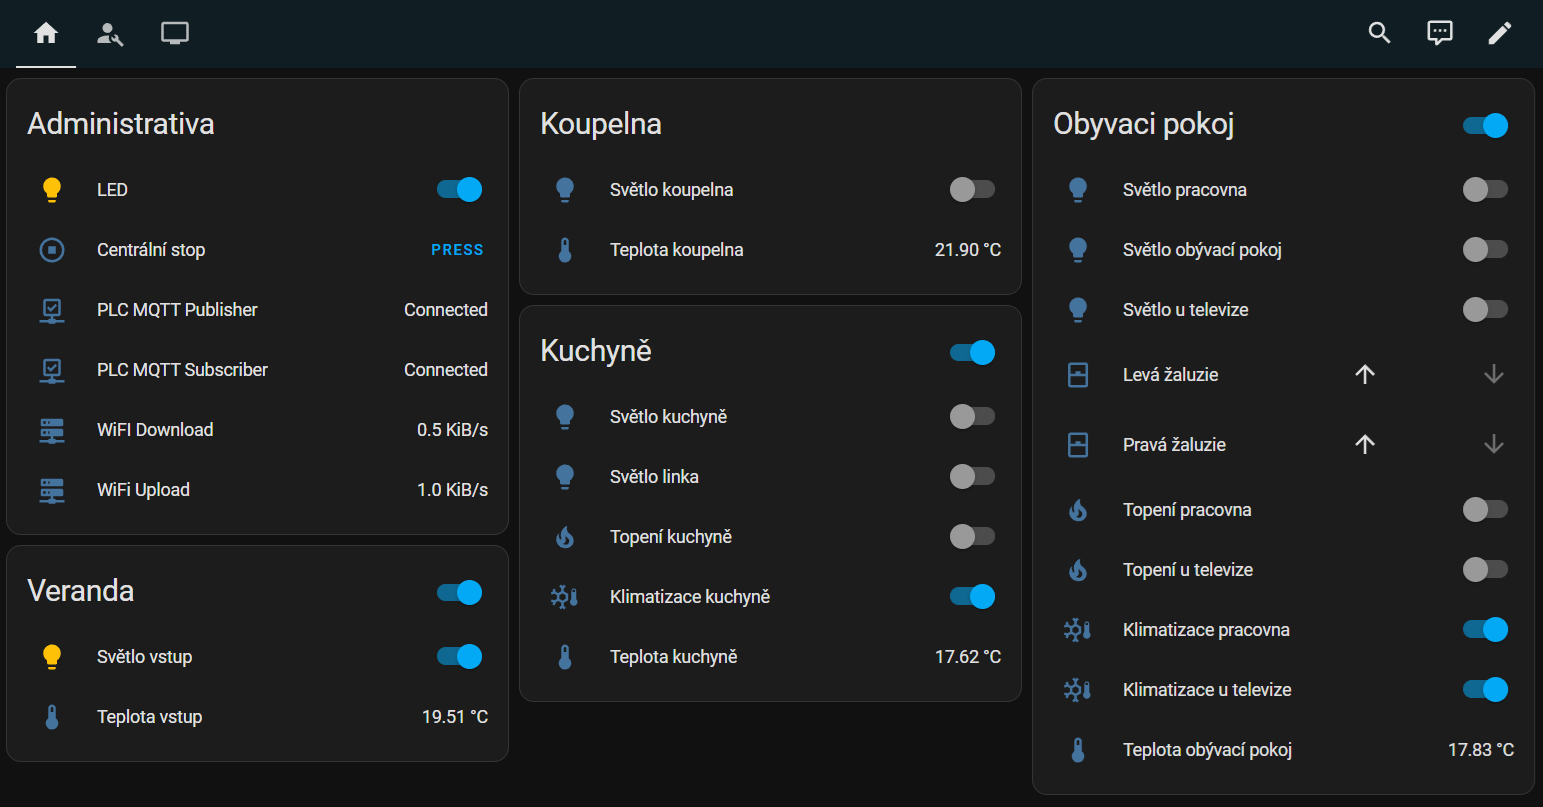
\includegraphics[scale=0.35]{obrazky/Dashboard1.png}
    \end{center}
    \caption[Home Assistant hrubá vizualizace]{Home Assistant hrubá vizualizace}
    \label{fig:HAvisu1}
\end{figure}

Pro jednodušší ovládání a přehlednost byly vytvořeny vlastní vizualizace. První byla vytvořena podle skupin ovládaných prvků (Obr. \ref{fig:HAvisu2}), druhá byla vytvořena podle místností (Obr. \ref{fig:HAvisu3}). Dále na nich byly použity jiné možné vzhledy jednotlivých prvků, které nabízí základní verze Home Assistantu. Pro případ, že by se ani ty uživateli nelíbily, je možné otevřít vyskakovací okna jednotlivých prvků, které nabízí více možností ovládání. V těchto oknech lze také sledovat historii jednotlivých prvků.

\begin{figure}[!ht]
    \begin{center}
        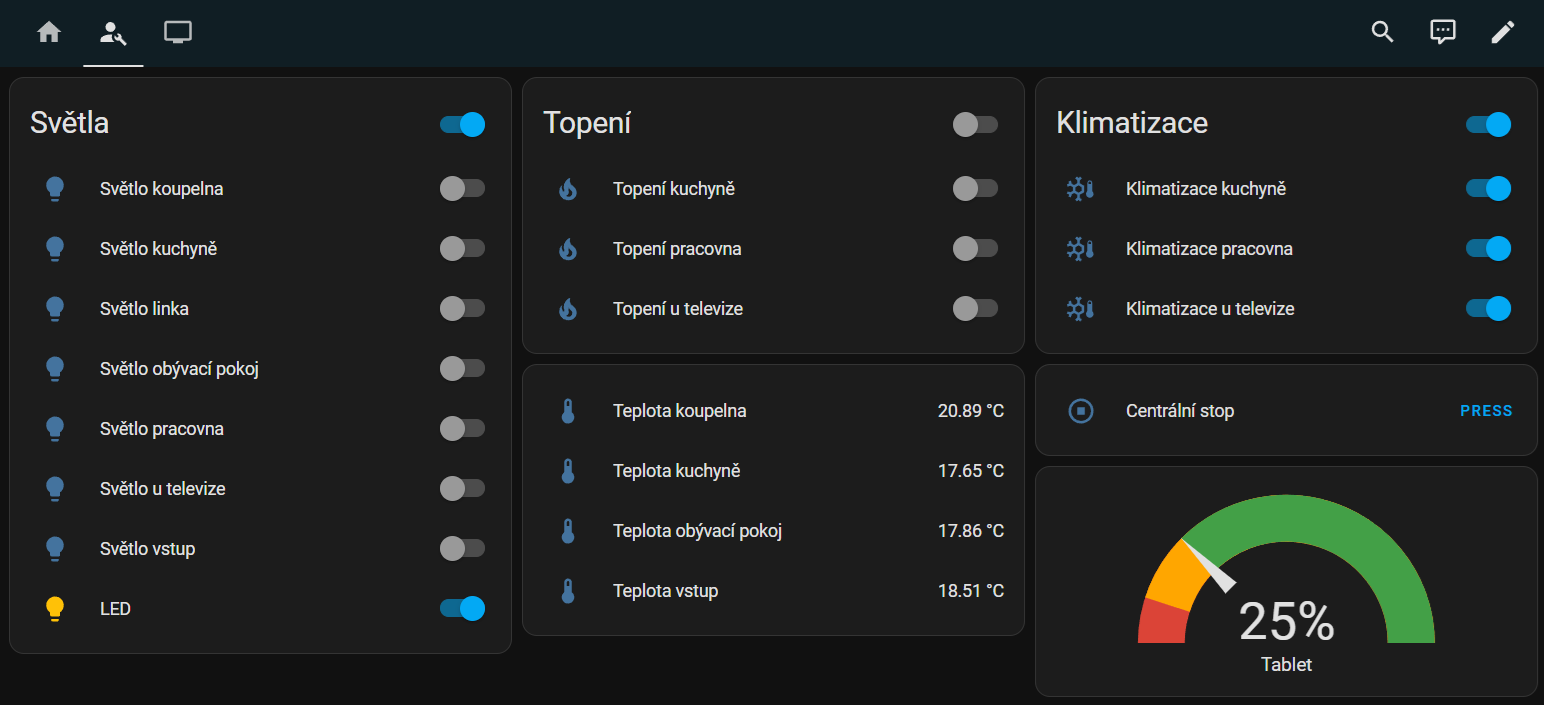
\includegraphics[scale=0.35]{obrazky/Dashboard2.png}
    \end{center}
    \caption[Home Assistant funkční vizualizace]{Home Assistant funkční vizualizace}
    \label{fig:HAvisu2}
\end{figure}

\begin{figure}[!ht]
    \begin{center}
        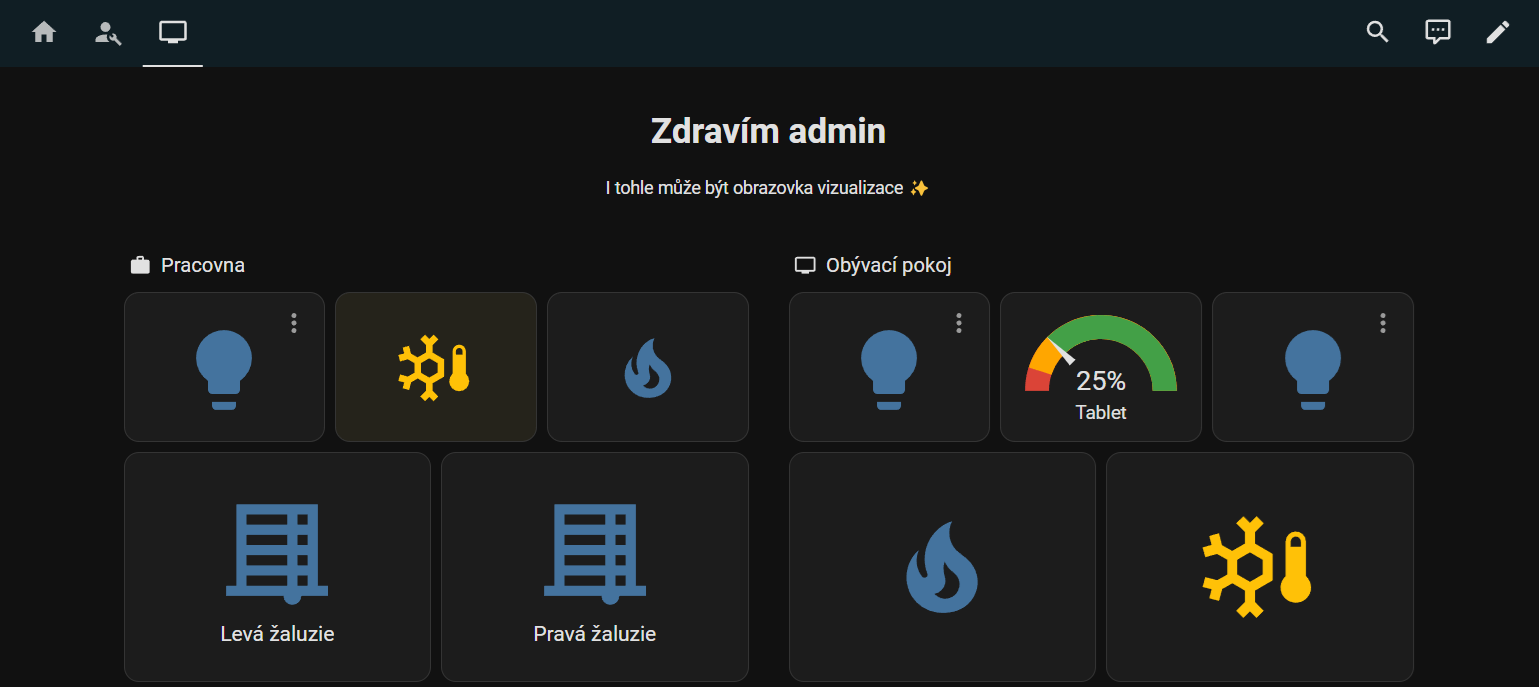
\includegraphics[scale=0.35]{obrazky/Dashboard3.png}
    \end{center}
    \caption[Home Assistant vizualizace dle umístění]{Home Assistant vizualizace dle umístění}
    \label{fig:HAvisu3}
\end{figure}

Pro potřebu sledování historie jednotlivých zařízení je možné použít vestavěnou funkci Home Assistantu - \textit{History}, která zobrazuje blízkou historii. Pro sledování delší historie bohužel neexistuje adekvátní řešení, protože Home Assistant ukládá historii do SQLite databáze, která není určena pro dlouhodobé ukládání dat. Proto byla použita integrace \textit{InfluxDB}. Další výhodou použití externí databáze je možnost sledovat historii i bez připojení k Home Assistantu. 

Připojení této databáze je uvedeno v příloze~\ref{apend:configyaml}.
\section{InfluxDB}
Jedná se o open-source databázi určenou pro ukládání časových řad. Databáze je optimalizována pro čtení a zápis velkého množství dat, která se následně využívají k analýze v reálném čase. Její hlavní výhodou je rychlost a efektivita při práci s velkým množstvím dat. Pro udržení rychlosti byly implementovány retenční politiky, které určují, jak dlouho se data uchovávají a jakým způsobem se agregují. \cite{InfluxDB} \newline

Databáze je tvořena několika základními koncepty~\cite{InfluxDBKeyConcepts}:
\begin{itemize}
    \item \textbf{Bucket} – kontejner pro ukládání dat
    \item \textbf{Measurement} – popis dat ukládaných do bucketu
    \item \textbf{Series} – skupina bodů se stejným tagem a měřením
    \item \textbf{Point} – jednotkový záznam v bucketu
    \item \textbf{Field} – hodnota ukládaná do bucketu
    \item \textbf{Tag} – klíč používaný k identifikaci dat v bucketu
    \item \textbf{Timestamp} – časový údaj o uložení dat
    \item \textbf{Retention policy} – pravidlo pro uchovávání dat v bucketu
    \item \textbf{Continuous query} – dotaz, který se provádí automaticky v pravidelných intervalech.
\end{itemize}
Kontejner této databáze běží na portu 8086. Po vytvoření kontejneru je potřeba nastavit uživatelské jméno a heslo pro přístup do databáze. Dále je potřeba nastavit bucket, do kterého se budou ukládat data – základní informace, délku uchovávání, způsob agregace dat a přístup přes API. Všechny tyto informace se nastavují pomocí webového rozhraní.

Webové rozhraní také umožňuje vytvářet a spravovat uživatelské účty a přístupová práva, sledovat výkon databáze, historii jednotlivých dat a vytvářet pro ně dotazy, které se provádějí pomocí jazyka \textit{Flux}. Tyto dotazy slouží k analýze dat a vytváření grafů, a to buď přímo v InfluxDB, nebo pomocí externích nástrojů, jako je Grafana. 
\section{Grafana}
Grafana je open-source platforma pro vizualizaci a analýzu dat. Umožňuje uživatelům vytvářet interaktivní grafy, tabulky a panely pro zpracování dat z různých zdrojů a také nastavovat upozornění na základě těchto dat. Disponuje širokým portfoliem pluginů, které umožňují připojení k různým databázím a službám. Grafana je velmi populární mezi vývojáři a administrátory, kteří potřebují monitorovat a analyzovat data v reálném čase. \cite{Grafana} \newline

Vizualizace v Grafaně je tvořena pomocí přehledů (dashboardů), které obsahují panely. Tyto panely mohou mít různé typy grafů~\cite{GrafanaVisualization}:
\begin{itemize}
    \item \textbf{Grafy a diagramy}
    \begin{itemize}
        \item \textbf{Time series} – data v čase
        \item \textbf{State timeline} – stav v čase
        \item \textbf{Status history} – periodický stav v čase
        \item \textbf{Bar chart} – kategoriální data
        \item \textbf{Histogram} – rozložení dat prezentované jako sloupcový graf
        \item \textbf{Heatmap} – vizualizace dat ve dvou rozměrech, typicky velikosti jevu
        \item \textbf{Pie chart} – zobrazení proporcionality
        \item \textbf{Candlestick} – typicky pro finanční data
        \item \textbf{Gauge} – zaoblený ukazatel zobrazující, jak daleko je metrika od prahu
        \item \textbf{Trend} – datové sady se sekvenčním, číselným x, které není čas
        \item \textbf{XY chart} – vizualizace hodnot x a y v grafu
    \end{itemize}
    \item \textbf{Statistika a čísla}
    \begin{itemize}
        \item \textbf{Stat} – velké statistiky a změny v čase
        \item \textbf{Bar gauge} – horizontální nebo vertikální ukazatel
    \end{itemize}
    \item \textbf{Různé}
    \begin{itemize}
        \item \textbf{Table} – vizualizace dat v tabulce
        \item \textbf{Logs} – vizualizace pro protokoly
        \item \textbf{Node graph} – orientované grafy nebo sítě
        \item \textbf{Traces} – trasování
        \item \textbf{Flame graph} – profilování
        \item \textbf{Canvas} – explicitní umístění prvků do statických a dynamických rozvržení
        \item \textbf{Geomap} – geoprostorová data
        \item \textbf{Datagrid} – vytváření a manipulace s daty (slouží jako zdroj dat pro jiné panely)
    \end{itemize}
    \item \textbf{Widgety}
    \begin{itemize}
        \item \textbf{Dashboard list} – seznam přehledů
        \item \textbf{Alert list} – seznam upozornění
        \item \textbf{Annotations list} – seznam anotací
        \item \textbf{Text} – markdown a HTML
        \item \textbf{News} – RSS kanály \newline
    \end{itemize}
\end{itemize}
Stejně jako v předchozích podkapitolách je i zde možné vytvářet a spravovat uživatelské účty a přístupová práva prostřednictvím webového rozhraní, tentokrát na portu 3000. \newline

\noindent Grafana v této práci sloužila jako nástroj pro zpracování historických dat instalace, konkrétně pro sledování spotřeby energie, jejího rozložení, měsíčních nákladů a historie sepnutí jednotlivých zařízení. Implementace a vzhled jednotlivých grafů jsou uvedeny v příloze \ref{apend:grafana}. 

%%% Vložení souboru 'text/zaver' se závěrem
\chapter*{Závěr}
\phantomsection
\addcontentsline{toc}{chapter}{Závěr}

V rámci této bakalářské práce byly splněny všechny stanovené cíle týkající se návrhu a realizace vzdáleného řízení a vizualizace demonstračního panelu KNX pro ovládání funkcí osvětlení, žaluzií, topení a klimatizace. Práce poskytuje ucelený pohled na problematiku sběrnicového systému KNX, jeho možnosti a praktické využití v oblasti domácí automatizace. 

V první části práce byla provedena důkladná analýza technologie KNX, včetně její historie, základních principů fungování, struktury komunikace, zabezpečení a topologie. Tato část poskytla nezbytný teoretický základ pro následnou praktickou realizaci. 

Druhá část práce se zaměřila na parametrizaci konkrétních přístrojů a tvorbu dynamických světelných scén. Byly popsány jednotlivé kroky od návrhu projektu až po jeho implementaci, včetně identifikace problémů. 

Třetí část práce se věnovala samotnému řízení a vizualizaci prostřednictvím PLC společnosti TECO. Popsány byly nejen technické aspekty programování a komunikace mezi PLC a KNX, ale také implementace MQTT protokolu a tvorba webové vizualizace. V této části práce vznikl problém těsně před jejím dokončením – došlo k poruše komunikační brány KNX IP BAOS 774. To mělo za následek nefunkčnost komunikace mezi PLC a KNX instalací. Situace je nyní řešena s technickou podporou a v nejhorším případě bude nutné vyměnit celou bránu.

V poslední části byly zhodnoceny možnosti využití open-source platforem pro vizualizaci a správu domácí automatizace. Byla provedena implementace na jednodeskovém počítači Raspberry Pi s využitím kontejnerizace Docker a nasazením několika open-source nástrojů, jako jsou Home Assistant, InfluxDB či Grafana. Tyto nástroje byly vybrány a nasazeny s ohledem na jejich aktuální popularitu, dostupnost a možnosti rozšíření.

Celkově lze konstatovat, že práce splnila vytyčené cíle a přinesla komplexní řešení vzdáleného řízení a vizualizace KNX panelu. Byly ověřeny možnosti integrace různých technologií a platforem, přičemž důraz byl kladen na praktičnost, flexibilitu a budoucí rozšiřitelnost řešení. Výsledky práce mohou sloužit jako inspirace či základ pro další rozvoj v oblasti chytré domácnosti a automatizace budov.


%%% Vložení souboru 'text/literatura' se seznamem zdrojů
% Pro sazbu seznamu literatury použijte jednu z následujících možností

%%%%%%%%%%%%%%%%%%%%%%%%%%%%%%%%%%%%%%%%%%%%%%%%%%%%%%%%%%%%%%%%%%%%%%%%%
%1) Seznam citací definovaný přímo pomocí prostředí literatura / thebibliography
\begin{thebibliography}{99}

\bibitem{Datapoint}
    	Asociace KNX \emph{Datapoint Type}\/ Online. 
    	Dostupné z:
    \url{https://support.knx.org/hc/en-us/articles/115001133744-Datapoint-Type}
    [cit.\,23.\,12.\,2021]. 
    
\bibitem{KNX history}
		Asociace KNX 
		\emph{A History of KNX}\/ Online.
		Dostupné z:
    \url{https://crelectrics.com.au/wp-content/uploads/2015/05/a_history_of_KNX.pdf}  
    [cit.\,1.\,10.\,2021]. 
    
\bibitem{KNX basics}
		Asociace KNX
		\emph{KNX Basics}\/ Online.
		Dostupné z:
    \url{https://www.knx.org/wAssets/docs/downloads/Marketing/Flyers/KNX-Basics/KNX-Basics_cz.pdf} 
		[cit.\,1.\,10.\,2021].
    
\bibitem{KNX principles}
    	Asociace KNX \emph{Principy systému KNX}\/ Online. 
    	Dostupné z:
    \url{https://knxcz.cz/images/clanky/KNX-System-Principles_cz.pdf} 
    	[cit.\,1.\,10.\,2021].
    
\bibitem{KNX Secure}
    	Asociace KNX \emph{KNX Secure Devices}\/ Online. 
    	Dostupné z:
    \url{https://support.knx.org/hc/en-us/articles/360000216419-KNX-Secure-Devices} 
    	[cit.\,23.\,12.\,2021].
    
\bibitem{Celkovy prehled}
    Asociace KNX \emph{ISO/IEC 14543-3. KNX Celkový přehled.}
    
\bibitem{Systemove Argumenty}
    Asociace KNX \emph{ISO/IEC 14543-3. KNX Systémové argumenty.}
    
\bibitem{Topologie}
    Asociace KNX \emph{ISO/IEC 14543-3. KNX TP Topologie.}
    
\bibitem{Mitrenga}
    MITRENGA, Michal.:
    \emph{Realizace demonstrativního panelu inteligentní elektroinstalace KNX. Brno, 2021.}\/ Online. 
    [cit. 26.\,12.\,2021].
    Dostupné z:
    \url{https://www.vutbr.cz/studenti/zav-prace/detail/134788}
    \emph{Diplomová práce. Vysoké učení technické v Brně, Fakulta elektrotechniky a komunikačních technologií, Ústav automatizace a měřicí techniky. Vedoucí práce Petr Fiedler.}
 
% \bibitem{Kalfus}
%    KALFUS, Petr..:
%    \emph{Návrh demonstračního panelu KNX. Brno, 2020.}\/ Online. 
%  [cit. 29.\,12.\,2021].
%   Dostupné z:
%    \url{https://www.vutbr.cz/studenti/zav-prace/detail/127255}   
%    \emph{Bakalářská práce. Vysoké učení technické v Brně, Fakulta elektrotechniky a komunikačních technologií, Ústav elektroenergetiky. Vedoucí práce Branislav Bátora.}

\bibitem{Asociace KNX}
		knx.org\/ Online.
		Dostupné z:
    \url{https://www.knx.org}
		[cit.\,1.\,10.\,2021]. 
    
\bibitem{ETS Kecy}
		knx.org \emph{ETS Professional}\/ Online.
		Dostupné z:
    \url{https://www.knx.org/knx-en/for-professionals/software/ets-professional/}
		[cit.\,2.\,1.\,2022]. 

\bibitem{KNXTunnel}
		Asociace KNX \emph{System Specifications KNXnet/IP - Tunelling}\/ Online.
		Dostupné z:
	\url{https://community-openhab-org.s3-eu-central-1.amazonaws.com/original/2X/8/8b3ec554f60872e37763d2005edc1c4c1fb16887.PDF}
		[cit.\,5.\,5.\,2025].

\bibitem{KNXRouting}
		Asociace KNX \emph{System Specifications - KNXnet/IP - Routing}\/ Online.
		Dostupné z:
	\url{https://community-openhab-org.s3-eu-central-1.amazonaws.com/original/2X/b/ba93de8a703a5ece40f0dfc1b596643cb28e8497.PDF}
		[cit.\,5.\,5.\,2025].

\bibitem{ABB}
		ABB - SBR/U6.0.1-84\/ Online. 
		Dostupné z:
    \url{https://new.abb.com/products/2CKA006330A0004/sbr-u6-0-1-84}
		[cit.\,28.\,12.\,2021].
    
\bibitem{ABB aktor1}
		ABB - SA/S8.10.2.1\/ Online.
		Dostupné z:
    \url{https://new.abb.com/products/2CDG110157R0011/sa-s8-10-2-1}
		[cit.\,28.\,12.\,2021]. 
    
\bibitem{ABB aktor2}
		ABB - JRA/S4.230.2.1\/ Online. 
		Dostupné z:
    \url{https://new.abb.com/products/2CDG110121R0011/jra-s4-230-2-1}
		[cit.\,28.\,12.\,2021].
    
\bibitem{Basalte}
		Basalte - Sentido aluminium - quad - Brushed black\/ Online.
		Dostupné z:
    \url{https://www.knxstore.cz/domu/1000403-basalte-sentido-aluminium-quad-brushed-black-5425025030224.html}
		[cit.\,28.\,12.\,2021]. 
    
 \bibitem{BEG}
		B.E.G - Indoor 140-L-KNX-DX\/ Online. 
		Dostupné z:
    \url{https://www.beg-luxomat.com/cz/produkty/luxomatnet/knx/knx-gen6-deluxe-pritomnostni-detektor/indoor-140-l-knx-dx/}
		[cit.\,28.\,12.\,2021].  
    
\bibitem{Berker}
		Berker - B.IQ push-button 3gang with thermostat Display, KNX\/ Online. 
		Dostupné z:
    \url{https://www.berker.com/en/e-catalogue/building-management-systems/knx-systems/berker-knx-system/b.iq-push-buttons-with-thermostat/75663593/355802.htm?lang=en}
		[cit.\,28.\,12.\,2021].
    
\bibitem{Ekinex}
		EKINEX - Pushbutton with thermostat\/ Online. 
		Dostupné z:
    \url{https://www.ekinex.com/en/15/pushbutton-with-thermostat.html}
		[cit.\,28.\,12.\,2021].
    
\bibitem{HDL}
        HDL - M/TBP6.1-A2-46 \textit{Ovládací prvek 6násobný iTouch, bílá}\/ Online. 
		Dostupné z:
    \url{https://b2b.hdl-automation.cz/cz/produkty/knx/ovladaci-prvky-hdl/ovladaci-prvky-itouch/hdl-m-tbp6-1-a2-46}
		[cit.\,28.\,12.\,2021].
    
\bibitem{HDL aktor1}
        HDL - M/R8.10.1 \textit{8CH 10A High Power Switch Actuator}\/ Online. 
		Dostupné z:
    \url{https://b2b.hdl-automation.cz/en/products/knx/switching-actuators/hdl-m-r8-10-1}
		[cit.\,28.\,12.\,2021].
    
\bibitem{HDL aktor2}
        HDL - M/DRGW4.1 \textit{Akční člen stmívací LED 4násobný, 7 A}\/ Online. 
		Dostupné z:
    \url{https://b2b.hdl-automation.cz/cz/produkty/knx/akcni-cleny-stmivaci/hdl-m-drgbw4-1}
		[cit.\,28.\,12.\,2021].
    
\bibitem{Siemens}
		SIEMENS - QMX3.P37 \textit{Prostorový KNX přístroj, displej pro regulaci HVAC, čidlo teploty, konfigurovatelná tlačítka pro osvětlení/žaluzie/scény}\/ Online. 
		Dostupné z:
    \url{https://hit.sbt.siemens.com/RWD/app.aspx?RC=CZ&lang=cs&MODULE=Catalog&ACTION=ShowProduct&KEY=S55624-H108}
		[cit.\,28.\,12.\,2021].
    
\bibitem{Siemens IP}
		SIEMENS - 5WG1 146-1AB03 \/ Online. 
		Dostupné z:
    \url{https://www.hqs.sbt.siemens.com/cps_product_data/data/search_find_en.htm?ssn=5WG11461AB03}
		[cit.\,28.\,12.\,2021].  
    
\bibitem{Simon}
		Simon \emph{Standard button box 4 functions white Simon 82 Sense}\/ Online. 
		Dostupné z:
    \url{https://www.simonelectric.com/intl/8000641-030-standard-button-box-4-functions-white-simon-82-sense.html}
		[cit.\,28.\,12.\,2021].

\bibitem{Weinzier}
		Weinzier - KNX IP BAOS 774\/ Online. 
		Dostupné z:
    \url{https://www.weinzierl.de/index.php/en/all-knx/knx-devices-en/knx-ip-baos-774-en}
		[cit.\,28.\,12.\,2021].
    
\bibitem{Weinzier ob}
		Weinzier - KNX IP BAOS 774 \emph{Rozhraní BAOS do 1000 bodů}\/ Online. 
		Dostupné z:
    \url{https://knx-trade.ru/weinzierl/597-5263.html}
		[cit.\,28.\,12.\,2021].

\bibitem{TECO}
		TECO - CP-2007\/ Online. 
		Dostupné z:
	\url{hhttps://wiki.tecomat.cz/clanek/cp-2007}
		[cit.\,23.\,4.\,2025].

\bibitem{Mosaic}
		TECO - Mosaic\/ Online. 
		Dostupné z:
	\url{https://www.tecomat.cz/ke-stazeni/software/mosaic/}
		[cit.\,23.\,4.\,2025].

\bibitem{IEC61131-3}
		TECO \emph{Programování PLC podle normy IEC 61 131-3 v prostředí Mosaic}\/ Online. 
		Dostupné z:
	\url{https://catalog.tecomat.cz/produkt/programovani-dle-normy-iec-61-131#download}
		[cit.\,23.\,4.\,2025].

\bibitem{KNXlib}
		TECO - Knihovna KnxLib\/ Online. 
		Dostupné z:
	\url{https://www.tecomat.cz/modules/DownloadManager/download.php?alias=txv00380_01}
		[cit.\,23.\,4.\,2025].

\bibitem{MQTT}
		MQTT \emph{The Standard for IoT Messaging}\/ Online. 
		Dostupné z:
	\url{https://mqtt.org}
		[cit.\,15.\,4.\,2025].

\bibitem{MQTTEsentials}
		MQTT Essentials \emph{The Ultimate Guide to MQTT for Beginners and Experts}\/ Online.
		Dostupné z:
		\url{https://www.hivemq.com/mqtt/}

\bibitem{JSON}
		JSON \emph{JavaScript Object Notation}\/ Online. 
		Dostupné z:
	\url{https://www.json.org/json-en.html}
		[cit.\,15.\,4.\,2025].

\bibitem{MQTTlib}
		TECO - Knihovna MQTTLib\/ Online. 
		Dostupné z:
	\url{https://support.tecomat.cz/storage/app/uploads/public/633/acd/862/633acd8625f3d859405244.pdf}
		[cit.\,23.\,4.\,2025].

\bibitem{WebMaker}
		TECO - WebMaker\/ Online. 
		Dostupné z:
	\url{https://www.tecomat.cz/modules/DownloadManager/download.php?alias=txv00328_01_mosaic_webmaker_cz}
		[cit.\,23.\,4.\,2025].

\bibitem{Flaticon}
		Flaticon \emph{The most wanted free SVG user interface icons}\/ Online. 
		Dostupné z:
	\url{https://www.flaticon.com/}
		[cit.\,5.\,5.\,2025].

\bibitem{Raspberry Pi 5}
		Raspberry Pi \emph{Raspberry Pi 5}\/ Online. 
		Dostupné z:
	\url{https://www.raspberrypi.com/products/raspberry-pi-5/}
		[cit.\,5.\,5.\,2025].

\bibitem{wear leveling}
		KIOXIA \emph{Managed Flash Background Operations Series - Part 3: Understanding Wear Leveling in NAND Flash Memory}\/ Online. 
		Dostupné z:
	\url{https://americas.kioxia.com/content/dam/kioxia/en-us/business/memory/mlc-nand/asset/KIOXIA_Managed_Flash_BOS_P3_Understanding_Wear_Leveling_Tech_Brief.pdf}
		[cit.\,5.\,5.\,2025].

\bibitem{Docker Compose}
		Docker Compose\/ Online. 
		Dostupné z:
	\url{https://docs.docker.com/compose/}
		[cit.\,5.\,5.\,2025].

\bibitem{DockerInstallationForDebian}
		Docker \emph{Docker Installation for Debian}\/ Online. 
		Dostupné z:
	\url{https://docs.docker.com/engine/install/debian/}
		[cit.\,5.\,5.\,2025].

\bibitem{ContainerAndVirtualization}
		Linux Containers \emph{Container and Virtualization tools}\/ Online.
		Dostupné z:
	\url{https://linuxcontainers.org}
		[cit.\,5.\,5.\,2025].

\bibitem{YAML}
		Yaml \emph{YAML Ain't Markup Language™}\/ Online. 
		Dostupné z:
	\url{hhttps://yaml.org/}
		[cit.\,5.\,5.\,2025].

\bibitem{ComposeYamlExample}
		Docker \emph{Compose file version 3 reference}\/ Online. 
		Dostupné z:
	\url{https://docs.docker.com/compose/compose-file/}
		[cit.\,5.\,5.\,2025].

\bibitem{ENV}
		Docker \emph{Environment variables}\/ Online. 
		Dostupné z:
	\url{https://docs.docker.com/engine/reference/run/#env}
		[cit.\,5.\,5.\,2025].

\bibitem{Portainer}
		Portainer\/ Online. 
		Dostupné z:
	\url{https://www.portainer.io/}
		[cit.\,5.\,5.\,2025].

\bibitem{Mosquitto}
		Eclipse Mosquitto\/ Online. 
		Dostupné z:
	\url{https://mosquitto.org/}
		[cit.\,15.\,5.\,2025].

\bibitem{Home Assistant}
		Home Assistant\/ Online. 
		Dostupné z:
	\url{https://www.home-assistant.io/}
		[cit.\,15.\,5.\,2025].

\bibitem{HACS}
		Home Assistant Community Store\/ Online. 
		Dostupné z:
	\url{https://hacs.xyz/}
		[cit.\,15.\,5.\,2025].

\bibitem{InfluxDB}
		InfluxDB\/ Online. 
		Dostupné z:
	\url{https://www.influxdata.com/}
		[cit.\,15.\,5.\,2025].

\bibitem{InfluxDBKeyConcepts}
		InfluxDB \emph{Key Concepts}\/ Online. 
		Dostupné z:
	\url{https://docs.influxdata.com/influxdb/v1/concepts/key_concepts/}
		[cit.\,15.\,5.\,2025].

\bibitem{Grafana}
		Grafana\/ Online. 
		Dostupné z:
	\url{https://grafana.com/}
		[cit.\,15.\,5.\,2025].

\bibitem{GrafanaVisualization}
		Grafana \emph{Visualizations}\/ Online. 
		Dostupné z:
	\url{https://grafana.com/docs/grafana/latest/panels-visualizations/visualizations/}
		[cit.\,15.\,5.\,2025].
\end{thebibliography} 
%%%%%%%%%%%%%%%%%%%%%%%%%%%%%%%%%%%%%%%%%%%%%%%%%%%%%%%%%%%%%%%%%%%%%%%%%
%%2) Seznam citací pomocí BibTeXu
%% Při použití je nutné v TeXnicCenter ve výstupním profilu aktivovat spouštění BibTeXu po překladu.
%% Definice stylu seznamu
%\bibliographystyle{unsrturl}
%% Pro českou sazbu lze použít styl czechiso.bst ze stránek
%% http://www.fit.vutbr.cz/~martinek/latex/czechiso.tar.gz
%%\bibliographystyle{czechiso}
%% Vložení souboru se seznamem citací
%\bibliography{text/literatura}
%
%% Následující příkaz je pouze pro ukázku sazby literatury při použití BibTeXu.
%% Způsobí citaci všech zdrojů v souboru literatura.bib, i když nejsou citovány v textu.
%\nocite{*}

%%% Vložení souboru 'text/zkratky' se seznam použitých symbolů, veličin a zkratek
\cleardoublepage
\chapter*{\listofabbrevname}
\phantomsection
\addcontentsline{toc}{chapter}{\listofabbrevname}

\begin{acronym}[KolikMista]

	\acro{zkTemp}		% název
		[Šířka levého sloupce Seznamu symbolů a zkratek]								% zkratka
		{je určena šířkou parametru prostředí \texttt{acronym} (viz řádek~1 výpisu zdrojáku na~str.\,\pageref{lst:zkratky})}
											% rozvinutí zkratky

	\acro{zkDummy}
		[KolikMista]
		{pouze ukázka vyhrazeného místa}

	\acro{DSP}		% název/zkratka
		{číslicové zpracování signálů -- Digital Signal Processing}
											% rozvinutí zkratky
	%%% bsymfvz
	\acro{symfvz}						% název
		[\ensuremath{f_\textind{vz}}] % symbol
		{vzorkovací kmitočet}					% popis
	%%% esymfvz

\end{acronym}


%%% Začátek příloh
\appendix

%%% Vysázení seznamu příloh
% (vynechejte, pokud máte dvě nebo méně příloh)
\listofappendices

%%% Vložení souboru 'text/prilohy' s přílohami
% Obvykle je přítomen alespoň popis co najdeme na přiloženém médiu
\chapter{Skupinové adresy}
\label{apend:skupinove_adresy}

\includepdf[pages = 1]{pdf/GroupAddressesReport}

\includepdf[pages = 2]{pdf/GroupAddressesReport}

\includepdf[pages = 3]{pdf/GroupAddressesReport}

\includepdf[pages = 4]{pdf/GroupAddressesReport}
\chapter{Definice funkčního bloku fbRoomTempMod}
\label{apend:fbRoomTempMod}
\begin{lstlisting}[language=ST, breaklines=true, numbers=left, numberstyle=\small, numbersep=10pt, frame=single, basicstyle=\ttfamily\small, caption={Definice funkčního bloku fbRoomTempMod}, label={lst:fbRoomTempMod}]
(*
FUNCTION_BLOCK fbRoomTempMod
(*Simulace změny teploty v pokojích*)
  VAR_INPUT
    Heat_1       : BOOl; // Topení vstup 1 [-]
    Heat_1_WATTS : REAL; // Topení výkon 1 [W] => [J/s]
    Heat_2       : BOOL; // Topení vstup 2 [-]
    Heat_2_WATTS : REAL; // Topení výkon 2 [W] => [J/s]
    Cold_1       : BOOl; // Klimatizace vstup 1 [-]
    Cold_1_WATTS : REAL; // Klimatizace výkon 1 [W] => [J/s]
    Cold_2       : BOOL; // Klimatizace vstup 2 [-]
    Cold_2_WATTS : REAL; // Klimatizace výkon 2 [W] => [J/s]
    lenght       : REAL; // délka [m]
    width        : REAL; // šířka [m]
    height       : REAL; // výška [m]
    wall_temp1   : REAL; // Teplota za sousední zdí [deg C]
    wall_temp2   : REAL; // Teplota za sousední zdí [deg C]
    wall_temp3   : REAL; // Teplota za sousední zdí [deg C]
    wall_temp4   : REAL; // Teplota za sousední zdí [deg C]
    floor_temp   : REAL; // Teplota v místnosti pod [deg C]
    ceiling_temp : REAL; // Teplota v místnosti nad [deg C]
    wall_thic1   : REAL; // Šířka zdi1 [m]
    wall_thic2   : REAL; // Šířka zdi2 [m]
    wall_thic3   : REAL; // Šířka zdi3 [m]
    wall_thic4   : REAL; // Šířka zdi4 [m]
    floor_thic   : REAL; // Šířka podlahy [m]
    ceiling_thic : REAL; // Šířka stropu [m]
    TaskTime     : REAL; // Rychlost tasku [ms]
  END_VAR
  VAR_OUTPUT
    Temperature  : REAL := 20.0; // Teplota na výstupu [deg C]
  END_VAR
  VAR_IN_OUT
  END_VAR
  VAR
    INIT         : BOOL := FALSE; //INIT bloku
    TimeStep     : REAL := 0.0; // Hodnota kroku v ms
    VAir         : REAL := 0.0; // Obsah vzduchu v pokoji [m^3]
    MAir         : REAL := 0.0;  // Váha vzduchu [Kg]
    QAir         : REAL := 0.0; // Energie potřebná ke změně o 1deg C [J]
    RoomTemp     : REAL := 20.0; // Pokojová teplota [deg C]
    DeltaTemp    : REAL := 0.0; // Přírůstek teploty za jeden cyklus [deg C]
    KHeatRise    : REAL := 2.4; // Korekční člen pro rychlosti náběhu topení 1 [-]
    KColdRise    : REAL := 45.0; // Korekční člen pro rychlosti náběhu klimatizace 1 [-]
    KHeatFall1   : REAL := 0.0; // Korekční člen pro rychlost poklesu topení 1 [-]
    KColdFall1   : REAL := 0.0; // Korekční člen pro rychlost poklesu klimatizace 1 [-]
    KHeatFall2   : REAL := 0.0; // Korekční člen pro rychlost poklesu topení 2 [-]
    KColdFall2   : REAL := 0.0; // Korekční člen pro rychlost poklesu klimatizace 2 [-]
    Epsilon      : REAL := 1.0; // Hodnota pod kterou musí být výkon do stanoveného času [-]
    AlphaHeat    : REAL := 0.0; // Výsledek logaritmu pro topení [-]
    AlphaCold    : REAL := 0.0; // Výsledek logaritmu pro klimatizace [-]
    FiTotal      : REAL := 0.0; // Celkový tepelný tok [J/s]
    FiHeat       : REAL := 0.0; // Celkový tepelný tok topení [J/s]
    FiHeatTmp1   : REAL := 0.0; // Tepelný tok topení 1 teď [J/s]
    FiHeatTmp2   : REAL := 0.0; // Tepelný tok topení 2 teď [J/s]
    FiCold       : REAL := 0.0; // Celkový tepelný tok klimatizace [J/s]
    FiColdTmp1   : REAL := 0.0; // Tepelný tok klimatizace 1 teď [J/s]
    FiColdTmp2   : REAL := 0.0; // Tepelný tok klimatizace 2 teď [J/s]
    AreaWall1    : REAL := 0.0; // Plocha zdi 1 [m^2]
    AreaWall2    : REAL := 0.0; // Plocha zdi 2 [m^2]
    AreaWall3    : REAL := 0.0; // Plocha zdi 3 [m^2]
    AreaWall4    : REAL := 0.0; // Plocha zdi 4 [m^2]
    AreaFloor    : REAL := 0.0; // Plocha podlahy [m^2]
    AreaCeiling  : REAL := 0.0; // Plocha stropu [m^2]
  END_VAR
  VAR_TEMP
    DeltaTempWall_1     : REAL := 0; // Rozdíl teplot mezi pokoji 1 [deg C]
    DeltaTempWall_2     : REAL := 0; // Rozdíl teplot mezi pokoji 2 [deg C]
    DeltaTempWall_3     : REAL := 0; // Rozdíl teplot mezi pokoji 3 [deg C]
    DeltaTempWall_4     : REAL := 0; // Rozdíl teplot mezi pokoji 4 [deg C]
    DeltaTempFloor      : REAL := 0; // Rozdíl teplot mezi pokojem a podlahou [deg C]
    DeltaTempCeiling    : REAL := 0; // Rozdíl teplot mezi pokojem a stropem [deg C]
    FiWall_1     : REAL := 0.0; // Tepelný tok mezi pokoji 1 [J/s]
    FiWall_2     : REAL := 0.0; // Tepelný tok mezi pokoji 2 [J/s]
    FiWall_3     : REAL := 0.0; // Tepelný tok mezi pokoji 3 [J/s]
    FiWall_4     : REAL := 0.0; // Tepelný tok mezi pokoji 4 [J/s]
    FiFloor      : REAL := 0.0; // Tepelný tok mezi pokojem a podlahou [J/s]
    FiCeiling    : REAL := 0.0; // Tepelný tok mezi pokojem a stropem [J/s]
  END_VAR
  VAR CONSTANT
    RoAir        : REAL := 1.204; // Hustota vzduchu [Kg/m^3]
    CpAir        : REAL := 1005.0; // Tepelná kapacita vzduchu [J/(kg*K)]
    LambdaBrick  : REAL := 0.4; // Tepelná vodivost cihly [W/(m*K)]
    MaxTemp      : REAL := 24.0; // Maximální teplota [deg C]
    MinTemp      : REAL := 16.0; // Minimální teplota [deg C]
    TimeRise     : REAL := 15.0; // Čas náběhu výkonu [s]
    TimeFallHeat : REAL := 15.0; // Čas klesání výkonu topení [s]
    TimeFallCold : REAL := 10.0; // Čas klesání výkonu klimatizace [s]
    TargTimeHeat : REAL := 5.06; // Čas na dosažení 80% topení [s]
    TargTimeCold : REAL := 3.29; // Čas na dosažení 80% klimatizace [s]
  END_VAR
IF NOT(INIT) THEN
   TimeStep := TaskTime / 1000.0; // ms => s
END_IF;
(* Výpočet objemu, hmotnosti, energie *)
IF NOT(INIT) THEN
  VAir := lenght * width * height;
  MAir := RoAir * VAir;
  QAir := MAir * CpAir;
END_IF;

(* Výpočet ploch *)
IF NOT(INIT) THEN
  AreaWall1 := height * width;
  AreaWall2 := height * width;
  AreaWall3 := height * lenght;
  AreaWall4 := height * lenght;
  AreaFloor := lenght * width;
  AreaCeiling := lenght * width;
END_IF;

(* Výpočet deltaT *)
DeltaTempWall_1 := wall_temp1 - RoomTemp;
DeltaTempWall_2 := wall_temp2 - RoomTemp;
DeltaTempWall_3 := wall_temp3 - RoomTemp;
DeltaTempWall_4 := wall_temp4 - RoomTemp;
DeltaTempFloor := floor_temp - RoomTemp;
DeltaTempCeiling := ceiling_temp - RoomTemp;

(* Výpočet tepelných toků přes stěny *)
FiWall_1 := (LambdaBrick * AreaWall1 * DeltaTempWall_1) / wall_thic1;
FiWall_2 := (LambdaBrick * AreaWall2 * DeltaTempWall_2) / wall_thic2;
FiWall_3 := (LambdaBrick * AreaWall3 * DeltaTempWall_3) / wall_thic3;
FiWall_4 := (LambdaBrick * AreaWall4 * DeltaTempWall_4) / wall_thic4;
FiFloor := (LambdaBrick * AreaFloor * DeltaTempFloor) / floor_thic;
FiCeiling := (LambdaBrick * AreaCeiling * DeltaTempCeiling) / ceiling_thic;

(* Výpočet korekčních členu *)
IF NOT(INIT) THEN
  KHeatRise := (TimeRise / TargTimeHeat) - 1.0;
  KColdRise := (TimeRise / TargTimeCold) - 1.0;

  KHeatFall1 := (LN(Heat_1_WATTS/Epsilon))/TimeFallHeat;
  KHeatFall2 := (LN(Heat_2_WATTS/Epsilon))/TimeFallHeat;
  KColdFall1 := (LN(Cold_1_WATTS/Epsilon))/TimeFallCold;
  KColdFall2 := (LN(Cold_2_WATTS/Epsilon))/TimeFallCold;
END_IF;

(* Tepelný výkon topení a klimatizace *)
(* Výpočet alfy *)
IF NOT(INIT) THEN
  AlphaHeat := LN(1 + KHeatRise * (TimeStep)) / LN(1 + KHeatRise * TimeRise);
  AlphaCold := LN(1 + KColdRise * (TimeStep)) / LN(1 + KColdRise * TimeRise);
END_IF;

(* Topení 1 *)
IF Heat_1 THEN
  FiHeatTmp1 := FiHeatTmp1 + AlphaHeat * (Heat_1_WATTS - FiHeatTmp1);
ELSE
  FiHeatTmp1 := FiHeatTmp1 * EXP(-KHeatFall1 * (TimeStep));
END_IF;

(* Topení 2 *)
IF Heat_2 THEN
  FiHeatTmp2 := FiHeatTmp2 + AlphaHeat * (Heat_2_WATTS - FiHeatTmp2);
ELSE
  FiHeatTmp2 := FiHeatTmp2 * EXP(-KHeatFall2 * (TimeStep));
END_IF;

(* Klimatizace 1 *)
IF Cold_1 THEN
  FiColdTmp1 := FiColdTmp1 + AlphaCold * (Cold_1_WATTS - FiColdTmp1);
ELSE
  FiColdTmp1 := FiColdTmp1 * EXP(-KColdFall1 * (TimeStep));
END_IF;

(* Klimatizace 2 *)
IF Cold_2 THEN
  FiColdTmp2 := FiColdTmp2 + AlphaCold * (Cold_2_WATTS - FiColdTmp2);
ELSE
  FiColdTmp2 := FiColdTmp2 * EXP(-KColdFall2 * (TimeStep));
END_IF;

(* Suma výkonů *)
FiHeat := FiHeatTmp1 + FiHeatTmp2;
FiCold := FiColdTmp1 + FiColdTmp2;

(* Celkový tepelný tok *)
FiTotal := FiHeat - FiCold + FiWall_1 + FiWall_2 + FiWall_3 + FiWall_4 + FiFloor + FiCeiling;

(* Výpočet přírůstku teploty za task *)
DeltaTemp := (FiTotal / QAir) * TimeStep;
RoomTemp := RoomTemp + DeltaTemp;

(* Výstup *)
Temperature := RoomTemp;

(* NOT INIT *)
INIT := TRUE;
END_FUNCTION_BLOCK
\end{lstlisting}
\newpage
\chapter{Popis funkčního bloku fbBath}
\label{apend:fbBath}
\begin{lstlisting}[language=ST, breaklines=true, numbers=left, numberstyle=\small, numbersep=10pt, frame=single, basicstyle=\ttfamily\small, caption={Definice funkčního bloku fbBath}, label={lst:fbBath}]
  FUNCTION_BLOCK fbBath
  VAR_INPUT
    SV6_ON       : BOOl; //Vizu světlo 6 on
    SV6_OFF      : BOOl; //Vizu světlo 6 off
    SV6_KNX_FB   : BOOl; //KNX světlo 6 feedback
  END_VAR
  VAR_OUTPUT
    SV6          : BOOL;   //Vizualizace světla 6
    SV6_CMD      : DT_CMD_BOOL;   //Příkaz světla 6
    TemperBath   : REAL;   //Vizualizace + komunikace
  END_VAR
  VAR_IN_OUT
  END_VAR
  VAR
    Time_s   : REAL := 0.0;
    fbSV6 : fbKNXVisuBool;
  END_VAR
  VAR_TEMP
  END_VAR
  VAR CONSTANT
    PI       : REAL := 3.14159265;
    Freq     : REAL := 0.005; // perioda cca 3 minuty 20 sekund
    TaskTime : REAL := 400.0; // 250 ms
  END_VAR
\end{lstlisting}
\begin{figure}[!ht]
  \begin{center}
  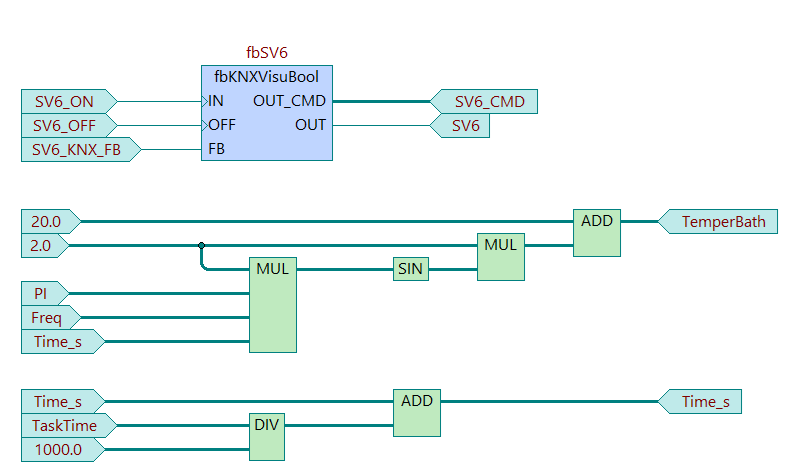
\includegraphics[scale=0.7]{obrazky/fbBath.png}
  \end{center}
  \caption[Logika funkčního bloku fbBath]{Logika funkčního bloku fbBath}
  \label{fig:fbBath}
\end{figure}
\pagebreak
\newpage
\chapter{Definice funkčního bloku fbKitch}
\label{apend:fbKitch}
\begin{lstlisting}[language=ST, breaklines=true, numbers=left, numberstyle=\small, numbersep=10pt, frame=single, basicstyle=\ttfamily\small, caption={Definice funkčního bloku fbKitch}, label={lst:fbKitch}]
  FUNCTION_BLOCK fbKitch
  VAR_INPUT
    SV1_ON         : BOOl; //Vizu světlo 1 on
    SV1_OFF        : BOOl; //Vizu světlo 1 off
    SV1_KNX_FB     : BOOl; //KNX světlo 1 feedback,
    SV2_ON         : BOOl; //Vizu světlo 2 on
    SV2_OFF        : BOOl; //Vizu světlo 2 off
    SV2_KNX_FB     : BOOl; //KNX světlo 2 feedback
    Heater3_ON     : BOOl; //Vizu topení 3 on
    Heater3_OFF    : BOOl; //Vizu topení 3 off
    Heater3_KNX_FB : BOOl; //KNX klimatizace 3 feedback
    Climat3_ON     : BOOl; //Vizu klimatizace 3 on
    Climat3_OFF    : BOOl; //Vizu klimatizace 3 off
    Climat3_KNX_FB : BOOl; //KNX topení 3 feedback
    wall_temp1     : REAL; // Teplota koupelna [deg C]
    wall_temp2     : REAL; // Teplota ven [deg C]
    wall_temp3     : REAL; // Teplota ven [deg C]
    wall_temp4     : REAL; // Teplota ven [deg C]
    ceiling_temp   : REAL; // Teplota obyvak [deg C]
  END_VAR
  VAR_OUTPUT
    SV1            : BOOL;   //Vizualizace světla 1
    SV2            : BOOL;   //Vizualizace světla 2
    Heater3        : BOOL;   //Vizualizace topení 3
    Climat3        : BOOL;   //Vizualizace klimatizace 3
    SV1_CMD        : DT_CMD_BOOL;   //Příkaz světla 1
    SV2_CMD        : DT_CMD_BOOL;   //Příkaz světla 2
    Heater3_CMD    : DT_CMD_BOOL;   //Příkaz topení 3
    Climat3_CMD    : DT_CMD_BOOL;   //Příkaz klimatizace 3
    TemperKitchen  : REAL;   //Vizualizace + komunikace
  END_VAR
  VAR_IN_OUT
  END_VAR
  VAR
    fbSV1 : fbKNXVisuBool;
    fbSV2 : fbKNXVisuBool;
    fbHeater3 : fbKNXVisuBool;
    fbKitchMod : fbRoomTempMod;
    fbClimat3 : fbKNXVisuBool;
  END_VAR
  VAR_TEMP
  END_VAR
\end{lstlisting}
\begin{figure}[!ht]
  \begin{center}
  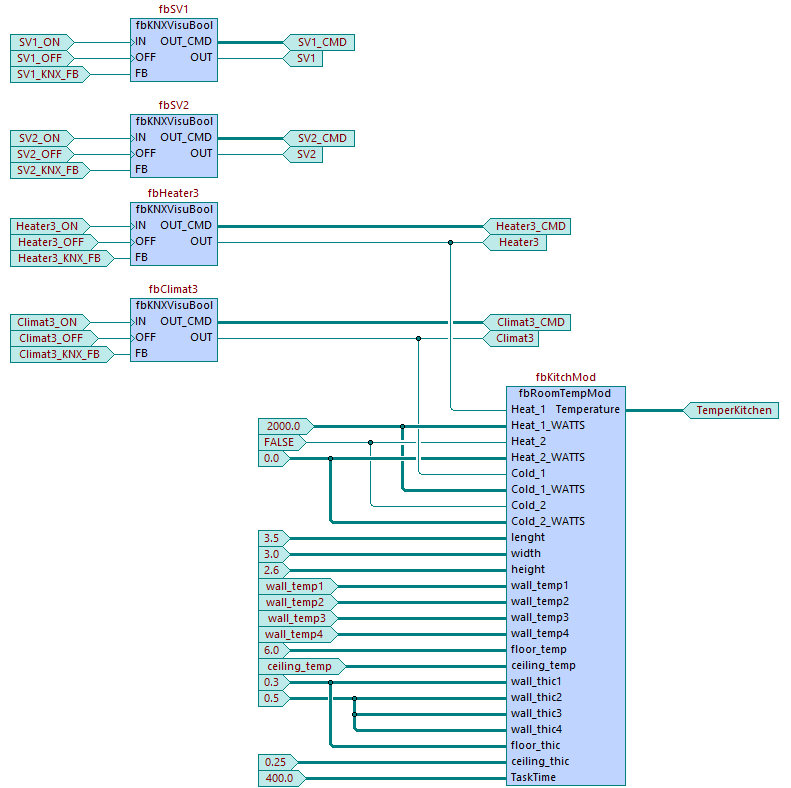
\includegraphics[scale=0.7]{obrazky/fbKitch.png}
  \end{center}
  \caption[Logika funkčního bloku fbKitch]{Logika funkčního bloku fbKitch}
  \label{fig:fbKitch}
\end{figure}
\pagebreak
\chapter{Definice funkčního bloku fbLivRoom}
\label{apend:fbLivRoom}
\begin{lstlisting}[language=ST, breaklines=true, numbers=left, numberstyle=\small, numbersep=10pt, frame=single, basicstyle=\ttfamily\small, caption={Definice funkčního bloku fbLivRoom}, label={lst:fbLivRoom}]
FUNCTION_BLOCK fbLivRoom
  VAR_INPUT
    SV3_ON          : BOOl; //Vizu světlo 3 on
    SV3_OFF         : BOOl; //Vizu světlo 3 off
    SV3_KNX_FB      : BOOl; //KNX světlo 3 feedback,
    SV4_ON          : BOOl; //Vizu světlo 4 on
    SV4_OFF         : BOOl; //Vizu světlo 4 off
    SV4_KNX_FB      : BOOl; //KNX světlo 4 feedback
    SV5_ON          : BOOl; //Vizu světlo 5 on
    SV5_OFF         : BOOl; //Vizu světlo 5 off
    SV5_KNX_FB      : BOOl; //KNX světlo 5 feedback
    Shut1_UP        : BOOl; //Vizu rolety 1 on
    Shut1_DW        : BOOl; //Vizu rolety 1 down
    Shut1_STEP_UP   : BOOl; //Vizu rolety 1 on krok
    Shut1_STEP_DW   : BOOl; //Vizu rolety 1 off krok
    Shut1_KNX_FB_UP : BOOl; //KNX rolety 1 feedback up
    Shut1_KNX_FB_DW : BOOl; //KNX rolety 1 feedback down
    Shut2_UP        : BOOl; //Vizu rolety 2 on
    Shut2_DW        : BOOl; //Vizu rolety 2 down
    Shut2_STEP_UP   : BOOl; //Vizu rolety 2 on krok
    Shut2_STEP_DW   : BOOl; //Vizu rolety 2 off krok
    Shut2_KNX_FB_UP : BOOl; //KNX rolety 2 feedback up
    Shut2_KNX_FB_DW : BOOl; //KNX rolety 2 feedback down
    Heater1_ON      : BOOl; //Vizu topení 1 on
    Heater1_OFF     : BOOl; //Vizu topení 1 off
    Heater1_KNX_FB  : BOOl; //KNX klimatizace 1 feedback
    Heater2_ON      : BOOl; //Vizu topení 2 on
    Heater2_OFF     : BOOl; //Vizu topení 2 off
    Heater2_KNX_FB  : BOOl; //KNX klimatizace 2 feedback
    Climat1_ON      : BOOl; //Vizu klimatizace 1 on
    Climat1_OFF     : BOOl; //Vizu klimatizace 1 off
    Climat1_KNX_FB  : BOOl; //KNX topení 1 feedback
    Climat2_ON      : BOOl; //Vizu klimatizace 2 on
    Climat2_OFF     : BOOl; //Vizu klimatizace 2 off
    Climat2_KNX_FB  : BOOl; //KNX topení 2 feedback
    wall_temp1      : REAL; // Teplota koupelna [deg C]
    wall_temp2      : REAL; // Teplota ven [deg C]
    wall_temp3      : REAL; // Teplota ven [deg C]
    wall_temp4      : REAL; // Teplota ven [deg C]
    floor_temp      : REAL; // Teplota v místnosti pod [deg C]
    ceiling_temp    : REAL; // Teplota obyvak [deg C]
  END_VAR
  VAR_OUTPUT
    SV3          : BOOL;   //Vizualizace světla 3
    SV4          : BOOL;   //Vizualizace světla 4
    SV5          : BOOL;   //Vizualizace světla 5
    SV3_CMD      : DT_CMD_BOOL;   //Příkaz světla 3
    SV4_CMD      : DT_CMD_BOOL;   //Příkaz světla 4
    SV5_CMD      : DT_CMD_BOOL;   //Příkaz světla 5
    Heater1        : BOOL;   //Vizualizace topení 1
    Heater2        : BOOL;   //Vizualizace topení 2
    Heater1_CMD    : DT_CMD_BOOL;   //Příkaz topení 1
    Heater2_CMD    : DT_CMD_BOOL;   //Příkaz topení 2
    Climat1        : BOOL;   //Vizualizace klimatizace 1
    Climat2        : BOOL;   //Vizualizace klimatizace 2
    Climat1_CMD    : DT_CMD_BOOL;   //Příkaz klimatizace 1
    Climat2_CMD    : DT_CMD_BOOL;   //Příkaz klimatizace 2
    Shut1_UP_OUT   : BOOL;   //Vizualizace žaluzie 1 UP
    Shut1_DOWN_OUT : BOOL;   //Vizualizace žaluzie 1 DOWN
    Shut1_CMD      : DT_CMD_BOOL;   //Příkaz žaluzie 1
    Shut1_STEP_CMD : DT_CMD_BOOL;   //Příkaz žaluzie 1 KROK
    Shut2_UP_OUT   : BOOL;   //Vizualizace žaluzie 2 UP
    Shut2_DOWN_OUT : BOOL;   //Vizualizace žaluzie 2 DOWN
    Shut2_CMD      : DT_CMD_BOOL;   //Příkaz žaluzie 2
    Shut2_STEP_CMD : DT_CMD_BOOL;   //Příkaz žaluzie 2 KROK
    TemperLivingR  : REAL;   //Vizualizace + komunikace
  END_VAR
  VAR_IN_OUT
  END_VAR
  VAR
    fbSV3 : fbKNXVisuBool;
    fbSV4 : fbKNXVisuBool;
    fbSV5 : fbKNXVisuBool;
    fbHeater1 : fbKNXVisuBool;
    fbClimat1 : fbKNXVisuBool;
    fbHeater2 : fbKNXVisuBool;
    fbClimat2 : fbKNXVisuBool;
    fbLivingRMod : fbRoomTempMod;
    fbShut1 : fbKNXShutters;
    fbShut2 : fbKNXShutters;
  END_VAR
  VAR_TEMP
  END_VAR
\end{lstlisting}
\begin{figure}[!ht]
  \begin{center}
  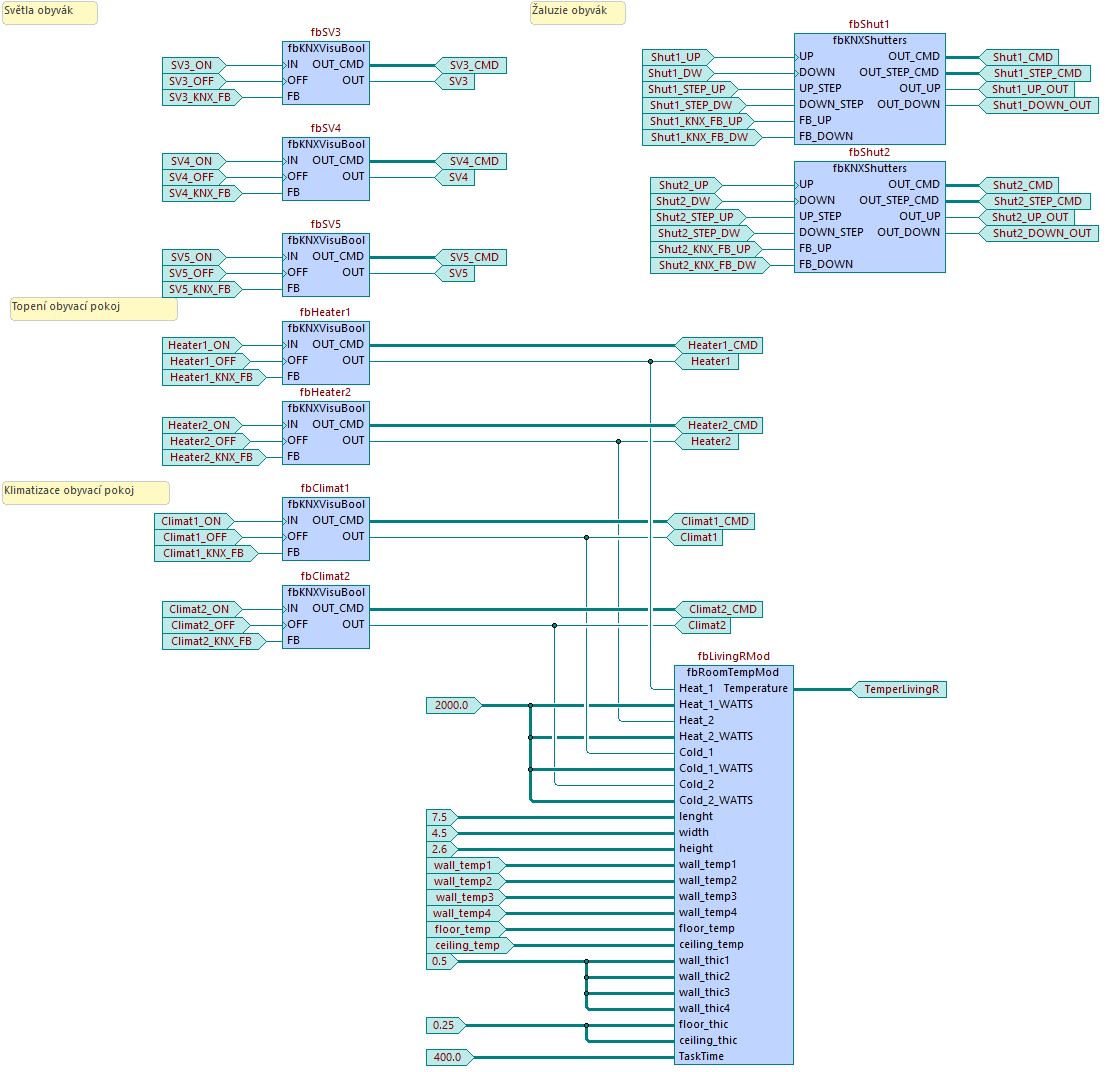
\includegraphics[scale=0.6]{obrazky/fbLivRoom.png}
  \end{center}
  \caption[Logika funkčního bloku fbLivRoom]{Logika funkčního bloku fbLivRoom}
  \label{fig:fbLivRoom}
\end{figure}
\pagebreak
\chapter{Definice funkčního bloku fbOutz}
\label{apend:fbOutz}
\begin{lstlisting}[language=ST, breaklines=true, numbers=left, numberstyle=\small, numbersep=10pt, frame=single, basicstyle=\ttfamily\small, caption={Definice funkčního bloku fbOutz}, label={lst:fbOutz}]
  FUNCTION_BLOCK fbOutz
  VAR_INPUT
    SV7_ON       : BOOl R_EDGE; //Vizu světlo 7 on
    SV7_OFF      : BOOl R_EDGE; //Vizu světlo 7 off
    SV7_KNX_FB   : BOOl; //KNX světlo 7 feedback
    KNX_OUT_TEMP : REAL; // KNX Teplota venku
  END_VAR
  VAR_OUTPUT
    SV7          : BOOL;   //Vizualizace světla 7
    SV7_CMD      : DT_CMD_BOOL;   //Příkaz světla 7
    TemperOut    : REAL;   //Vizualizace + komunikace
  END_VAR
  VAR_IN_OUT
  END_VAR
  VAR
    fbSV7 : fbKNXVisuBool;
  END_VAR
  VAR_TEMP
  END_VAR
\end{lstlisting}
\begin{figure}[!ht]
  \begin{center}
  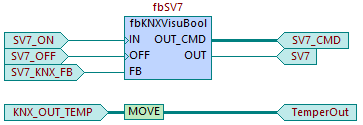
\includegraphics[scale=1.3]{obrazky/fbOutz.png}
  \end{center}
  \caption[Logika funkčního bloku fbOutz]{Logika funkčního bloku fbOutz}
  \label{fig:fbOutz}
\end{figure}
\pagebreak
\chapter{Program komunikace mezi PLC a KNX}
\label{apend:KNXComm}
\begin{lstlisting}[language=ST, breaklines=true, numbers=left, numberstyle=\small, numbersep=10pt, frame=single, basicstyle=\ttfamily\small, caption={Program komunikace mezi PLC a KNX}, label={lst:prgKNXComm}]
  PROGRAM prgKNXComm
  VAR_INPUT
  END_VAR
  VAR_OUTPUT
  END_VAR
  VAR
    init : BOOL;
    knx  : fbKnxIpBaosBin;
    
    SHUT1_FB_PULSE : TON;
    SHUT2_FB_PULSE : TON;

    datapoint1       : T_KNX_OBJECT_DPT1;     // SV1_FB
    datapoint2       : T_KNX_OBJECT_DPT1;     // SV2_FB
    datapoint3       : T_KNX_OBJECT_DPT1;     // SV3_FB
    datapoint4       : T_KNX_OBJECT_DPT1;     // SV4_FB
    datapoint5       : T_KNX_OBJECT_DPT1;     // SV5_FB
    datapoint6       : T_KNX_OBJECT_DPT1;     // SV6_FB
    datapoint7       : T_KNX_OBJECT_DPT1;     // SV7_FB

    datapoint8       : T_KNX_OBJECT_DPT1;     // HEAT1_FB
    datapoint9       : T_KNX_OBJECT_DPT1;     // HEAT2_FB
    datapoint10      : T_KNX_OBJECT_DPT1;     // HEAT3_FB

    datapoint11      : T_KNX_OBJECT_DPT1;     // COLD1_FB
    datapoint12      : T_KNX_OBJECT_DPT1;     // COLD2_FB
    datapoint13      : T_KNX_OBJECT_DPT1;     // COLD3_FB

    datapoint14      : T_KNX_OBJECT_DPT1;     // SHUT1_FB
    datapoint15      : T_KNX_OBJECT_DPT1;     // SHUT1_CMD
    datapoint16      : T_KNX_OBJECT_DPT1;     // SHUT2_FB
    datapoint17      : T_KNX_OBJECT_DPT1;     // SHUT2_CMD

    datapoint18      : T_KNX_OBJECT_DPT1;     // SV1_CMD
    datapoint19      : T_KNX_OBJECT_DPT1;     // SV2_CMD
    datapoint20      : T_KNX_OBJECT_DPT1;     // SV3_CMD
    datapoint21      : T_KNX_OBJECT_DPT1;     // SV4_CMD
    datapoint22      : T_KNX_OBJECT_DPT1;     // SV5_CMD
    datapoint23      : T_KNX_OBJECT_DPT1;     // SV6_CMD
    datapoint24      : T_KNX_OBJECT_DPT1;     // SV7_CMD

    datapoint25      : T_KNX_OBJECT_DPT1;     // HEAT1_CMD
    datapoint26      : T_KNX_OBJECT_DPT1;     // HEAT2_CMD
    datapoint27      : T_KNX_OBJECT_DPT1;     // HEAT3_CMD

    datapoint28      : T_KNX_OBJECT_DPT1;     // krok Žaluzií 1
    datapoint29      : T_KNX_OBJECT_DPT1;     // krok Žaluzií 2

    datapoint30      : T_KNX_OBJECT_DPT18;    // scéna
    datapoint31      : T_KNX_OBJECT_DPT9;     // teplota

    knxObjectList    : ARRAY[1..31] OF UDINT; // pole adres
  END_VAR
  VAR_TEMP
  END_VAR
  
// pole adres
IF NOT init THEN
  knxObjectList[1]  := PTR_TO_UDINT( ADR(datapoint1));   // SV1_FB
  knxObjectList[2]  := PTR_TO_UDINT( ADR(datapoint2));   // SV2_FB
  knxObjectList[3]  := PTR_TO_UDINT( ADR(datapoint3));   // SV3_FB
  knxObjectList[4]  := PTR_TO_UDINT( ADR(datapoint4));   // SV4_FB
  knxObjectList[5]  := PTR_TO_UDINT( ADR(datapoint5));   // SV5_FB
  knxObjectList[6]  := PTR_TO_UDINT( ADR(datapoint6));   // SV6_FB
  knxObjectList[7]  := PTR_TO_UDINT( ADR(datapoint7));   // SV7_FB

  knxObjectList[8]  := PTR_TO_UDINT( ADR(datapoint8));   // HEAT1_FB
  knxObjectList[9]  := PTR_TO_UDINT( ADR(datapoint9));   // HEAT2_FB
  knxObjectList[10] := PTR_TO_UDINT( ADR(datapoint10));  // HEAT3_FB

  knxObjectList[11] := PTR_TO_UDINT( ADR(datapoint11));  // COLD1_FB
  knxObjectList[12] := PTR_TO_UDINT( ADR(datapoint12));  // COLD2_FB
  knxObjectList[13] := PTR_TO_UDINT( ADR(datapoint13));  // COLD3_FB

  knxObjectList[14] := PTR_TO_UDINT( ADR(datapoint14));  // SHUT1_FB
  knxObjectList[15] := PTR_TO_UDINT( ADR(datapoint15));  // Zastarale
  knxObjectList[16] := PTR_TO_UDINT( ADR(datapoint16));  // SHUT2_FB
  knxObjectList[17] := PTR_TO_UDINT( ADR(datapoint17));  // Zastarale

  knxObjectList[18] := PTR_TO_UDINT( ADR(datapoint18));  // SV1_CMD
  knxObjectList[19] := PTR_TO_UDINT( ADR(datapoint19));  // SV2_CMD
  knxObjectList[20] := PTR_TO_UDINT( ADR(datapoint20));  // SV3_CMD
  knxObjectList[21] := PTR_TO_UDINT( ADR(datapoint21));  // SV4_CMD
  knxObjectList[22] := PTR_TO_UDINT( ADR(datapoint22));  // SV5_CMD
  knxObjectList[23] := PTR_TO_UDINT( ADR(datapoint23));  // SV6_CMD
  knxObjectList[24] := PTR_TO_UDINT( ADR(datapoint24));  // SV7_CMD

  knxObjectList[25] := PTR_TO_UDINT( ADR(datapoint25));  // HEAT1_CMD
  knxObjectList[26] := PTR_TO_UDINT( ADR(datapoint26));  // HEAT2_CMD
  knxObjectList[27] := PTR_TO_UDINT( ADR(datapoint27));  // HEAT3_CMD

  knxObjectList[28] := PTR_TO_UDINT( ADR(datapoint28));  // krok Žaluzie 1
  knxObjectList[29] := PTR_TO_UDINT( ADR(datapoint29));  // krok Žaluzie 2

  knxObjectList[30] := PTR_TO_UDINT( ADR(datapoint30));  // scéna
  knxObjectList[31] := PTR_TO_UDINT( ADR(datapoint31));  // teplota

  init := TRUE;
END_IF

knx( firstKnxObject := 1,
     lastKnxObject := 31,
     ethCode := ETH2_uni2,
     knxIP := STRING_TO_IPADR('192.168.xxx.xx'),
     knxList := void( knxObjectList));

// Feedbacky
SV1_FB       := datapoint1 .value;
SV2_FB       := datapoint2 .value;
SV3_FB       := datapoint3 .value;
SV4_FB       := datapoint4 .value;
SV5_FB       := datapoint5 .value;
SV6_FB       := datapoint6 .value;
SV7_FB       := datapoint7 .value;

HEAT1_FB     := datapoint8 .value;
HEAT2_FB     := datapoint9 .value;
HEAT3_FB     := datapoint10.value;

COLD1_FB     := datapoint11.value;
COLD2_FB     := datapoint12.value;
COLD3_FB     := datapoint13.value;

SHUT1_FB_PULSE(IN := datapoint14.altValue, PT := T#1s);
SHUT2_FB_PULSE(IN := datapoint16.altValue, PT := T#1s);

SHUT1_FB_UP   := datapoint14.value AND SHUT1_FB_PULSE.Q;
SHUT1_FB_DOWN := NOT(datapoint14.value) AND SHUT1_FB_PULSE.Q;
SHUT2_FB_UP   := datapoint16.value AND SHUT2_FB_PULSE.Q;
SHUT2_FB_DOWN := NOT(datapoint16.value) AND SHUT2_FB_PULSE.Q;

// Příkazy
IF SV1_CMD.CMD       THEN datapoint18.value := SV1_CMD.CMD_VAL; END_IF;
IF SV2_CMD.CMD       THEN datapoint19.value := SV2_CMD.CMD_VAL; END_IF;
IF SV3_CMD.CMD       THEN datapoint20.value := SV3_CMD.CMD_VAL; END_IF;
IF SV4_CMD.CMD       THEN datapoint21.value := SV4_CMD.CMD_VAL; END_IF;
IF SV5_CMD.CMD       THEN datapoint22.value := SV5_CMD.CMD_VAL; END_IF;
IF SV6_CMD.CMD       THEN datapoint23.value := SV6_CMD.CMD_VAL; END_IF;
IF SV7_CMD.CMD       THEN datapoint24.value := SV7_CMD.CMD_VAL; END_IF;

IF HEAT1_CMD.CMD     THEN datapoint25.value := HEAT1_CMD.CMD_VAL; END_IF;
IF HEAT2_CMD.CMD     THEN datapoint26.value := HEAT2_CMD.CMD_VAL; END_IF;
IF HEAT3_CMD.CMD     THEN datapoint27.value := HEAT3_CMD.CMD_VAL; END_IF;

IF SHUT1_CMD.CMD     THEN datapoint15.value  := SHUT1_CMD.CMD_VAL; END_IF;
IF SHUT1_STEP_CMD.CMD THEN datapoint28.value := SHUT1_STEP_CMD.CMD_VAL; END_IF;
IF SHUT2_CMD.CMD     THEN datapoint17.value  := SHUT1_CMD.CMD_VAL; END_IF;
IF SHUT2_STEP_CMD.CMD THEN datapoint29.value := SHUT1_STEP_CMD.CMD_VAL; END_IF;

// Shutdown scéna
IF SHUTDOWN_MQTT THEN
  datapoint30.control := TRUE;
  datapoint30.scene   := 5;
END_IF

// Posílání teploty
KNX_TEMPER := datapoint31.value;

END_PROGRAM
\end{lstlisting}
\end{document}